%% 
%% Copyright 2019-2021 Elsevier Ltd
%% 
%% This file is part of the 'CAS Bundle'.
%% --------------------------------------
%% 
%% It may be distributed under the conditions of the LaTeX Project Public
%% License, either version 1.2 of this license or (at your option) any
%% later version.  The latest version of this license is in
%%    http://www.latex-project.org/lppl.txt
%% and version 1.2 or later is part of all distributions of LaTeX
%% version 1999/12/01 or later.
%% 
%% The list of all files belonging to the 'CAS Bundle' is
%% given in the file `manifest.txt'.
%% 
%% Template article for cas-dc documentclass for 
%% double column output.

\documentclass[fleqn]{cas-sc}

\usepackage{lipsum}
\usepackage{tikz}
\usetikzlibrary{shapes, snakes, calc, positioning}
\usepackage{longtable}
\usepackage{enumitem}
\usepackage[section]{placeins}

% If the frontmatter runs over more than one page
% use the longmktitle option.

%\documentclass[a4paper,fleqn,longmktitle]{cas-dc}

%\usepackage[numbers]{natbib}
%\usepackage[authoryear]{natbib}
\usepackage[authoryear,longnamesfirst]{natbib}

%%%Author macros
\def\tsc#1{\csdef{#1}{\textsc{\lowercase{#1}}\xspace}}
\tsc{WGM}
\tsc{QE}
%%%

% Uncomment and use as if needed
%\newtheorem{theorem}{Theorem}
%\newtheorem{lemma}[theorem]{Lemma}
%\newdefinition{rmk}{Remark}
%\newproof{pf}{Proof}
%\newproof{pot}{Proof of Theorem \ref{thm}}

\begin{document}
\let\WriteBookmarks\relax
\def\floatpagepagefraction{1}
\def\textpagefraction{.001}

% Short title
\shorttitle{Ambulance Dispatch}    

% Short author
\shortauthors{Burkman, Chu, Jin, Abuhijleh, and Sun}  
%\shortauthors{First, Second, Third, Fourth}  

% Main title of the paper
\title [mode = title]{Ambulance Dispatch Recommendation System based on Automated Crash Reports from Cell Phones}  

% Title footnote mark
% eg: \tnotemark[1]
%\tnotemark[<tnote number>] 
%\tnotemark[1] 

% Title footnote 1.
% eg: \tnotetext[1]{Title footnote text}
%\tnotetext[1]{Working Title} 

% First author
%
% Options: Use if required
% eg: \author[1,3]{Author Name}[type=editor,
%       style=chinese,
%       auid=000,
%       bioid=1,
%       prefix=Sir,
%       orcid=0000-0000-0000-0000,
%       facebook=<facebook id>,
%       twitter=<twitter id>,
%       linkedin=<linkedin id>,
%       gplus=<gplus id>]

%\author[<aff no>]{<author name>}[<options>]
\author[1,2]{J. Bradford Burkman}[]
%\author[1,2]{First Author}[]
% Footnote of the first author
\fnmark[1]
% Corresponding author indication
\cormark[1]
% Email id of the first author
\ead{bradburkman@gmail.com}
%\ead{FirstAuthor@gmail.com}
% URL of the first author
\ead[url]{http://www.github.com/bburkman/Ambulance_Dispatch}

% Credit authorship
% eg: \credit{Conceptualization of this study, Methodology, Software}
% Options: conceptualization; data curation; formal analysis; funding acquisition; investigation; methodology; project administration; resources; software; supervision; validation; visualization; writing – original draft; and writing – review and editing.
\credit{Conceptualization, Investigation, Writing - original draft, Visualization}

\author[1]{Chee-Hung Henry Chu}
\credit{Supervision, Methodology, Writing - review and editing}

\author[1]{Miao Jin}[]
%\author[1]{Second Author}[]
\credit{Supervision, Methodology}

\author[1,3]{Malek Abuhijleh}[]
%\author[1,3]{Third Author}[]
\credit{Data curation, Investigation, Methodology}

\author[3]{Xiaoduan Sun}[]
%\author[3]{Fourth Author}[]
\credit{Data curation, Writing - review and editing}





\affiliation[1]{organization={School of Computing and Informatics, University of Louisiana at Lafayette},
%\affiliation[1]{organization={School, University},
            addressline={301 E. Lewis St}, 
            city={Lafayette},
          citysep={}, % Uncomment if no comma needed between city and postcode
            state={LA},
            postcode={70503}, 
            country={USA}
            }

% Address/affiliation
\affiliation[2]{organization={Louisiana School for Math, Science, and the Arts},
%\affiliation[2]{organization={Other School},
            addressline={715 University Pkwy}, 
            city={Natchitoches},
          citysep={}, % Uncomment if no comma needed between city and postcode
            state={LA},
            postcode={71457}, 
            country={USA}
            }

\affiliation[3]{organization={Department of Civil Engineering, University of Louisiana at Lafayette},
%\affiliation[3]{organization={Other Department, University},
            addressline={131 Rex St}, 
            city={Lafayette},
          citysep={}, % Uncomment if no comma needed between city and postcode
            state={LA},
            postcode={70504}, 
            country={USA}
            }




% For a title note without a number/mark
%\nonumnote{}

% Here goes the abstract
\begin{abstract}
%%%%% Abstract
% I found an abstract in TRpC June 2022 with 365 words.
%Put abstract here.
%%%%% Abstract
% I found an abstract in TRpC June 2022 with 365 words.
Some new cell phones can automatically notify an emergency dispatcher if the phone detects the deceleration profile of a vehicular crash.  Most crash notifications come from an eyewitness who can say whether an ambulance is needed, but the automated notification from the cell phone cannot provide that information directly.  Should the dispatcher immediately send an ambulance before receiving an eyewitness report?  There are three options: Always, Wait, and Sometimes.  The ``Always'' option refers to sending an ambulance to every automatically reported crash, even though most of them will not be needed.  In the ``Wait'' option, the dispatcher sends police, but always waits for a call from an eyewitness (perhaps the police) before sending an ambulance.  In the ``Sometimes'' option, the dispatcher has some system that recommends whether to immediately dispatch an ambulance, reserving the option to send one later based on an eyewitness report.

%This paper explores one option for building a machine learning (ML) model for making a recommendation in the ``Sometimes'' option.  The model gives the probability (based on the available information) that a crash requires an ambulance.  If the probability that an ambulance is needed is above some chosen threshold, the method will recommend dispatching an ambulance immediately; below that threshold, the dispatcher should wait to hear from an eyewitness. 


This paper explores one option for building a machine learning (ML) model for making a recommendation in the ``Sometimes'' option.    Our goal is to build a model that returns, for each feature vector (crash report, sample), a value $p \in [0,1]$ that increases with the probability that the person needs an ambulance.  Using a decision threshold $\theta$, we immediately send ambulances to those automated crash reports with $p > \theta$, and wait for eyewitness confirmation for those reports with $p < \theta$. In an actual implementation, the choice of $\theta$ is political, not technical.

The costs of the false positives (FP) and false negatives (FN) in dispatching ambulances are very different.  The cost of sending an ambulance when one is not needed (FP) is measured in dollars, but the cost of not promptly sending an ambulance when one is needed (FN) is measured in lives.  Choosing the decision threshold $\theta$ is ethically problematic, but governments make such a tradeoff when they set budgets for emergency services.  

We consider and interpret three options for the decision threshold $\theta$ based on the political consideration, ``How much will it cost?''  How many automated ambulance dispatches are we willing to fund (FP + TP) for each one of them that is actually needed (TP)?  We will explore two versions of that question, the total and the marginal.  


%some of which consider a relationship between the total number of FP and FN up to that value of $p$, and others consider the marginal relationship around that value of $p$.  Once the threshold criteria are chosen, the problem turns to choosing and tuning a model that best satisfies the tradeoff, saving both money and lives.  

%We consider the factors in determining the threshold.  The costs of the false positives (FP) and false negatives (FN) in dispatching ambulances are very different.  The cost of sending an ambulance when one is not needed (FP) is measured in dollars, but the cost of not promptly sending an ambulance when one is needed (FN) is measured in lives.  Choosing such a tradeoff threshold is ethically problematic, but governments implicitly make such a tradeoff when they set budgets for emergency and medical services.  To demonstrate the method in this paper, we have arbitrarily chosen a cutoff of 33\%, that there is a 1 in 3 chance that a dispatched ambulance would be needed (TP) and a 2 in 3 chance that it would not (FP).  We formulate our marginal ethical tradeoff rate as   $\omega = \Delta FP/\Delta TP = 2.0$.  We incorporated $\omega$ into the model in the class weight and in the decision threshold.  

We show that the quality of the model depends highly on the input data available, having considered three levels of data availability.  The ``Easy'' level includes data the emergency dispatcher has before the notification, like time of day and weather.  The ``Medium'' level adds information about the location and information from the cell service provider about the user, like the age and sex.  The ``Hard'' level adds information that requires having access to records about the vehicle likely to be driven by the cell phone user and detailed and temporal information about the location, like lighting conditions and whether it is currently a work zone.  

We used the data of the Crash Report Sampling System (CRSS) to validate our approach.  We have applied new methods (for this dataset in the literature) to handle missing data, and we have investigated several methods for handling the data imbalance.  To promote discussion and future research, we have included all of the code we used in our analysis.  
%\vskip 1in

\end{abstract}

% Use if graphical abstract is present
\begin{graphicalabstract}

{
\footnotesize
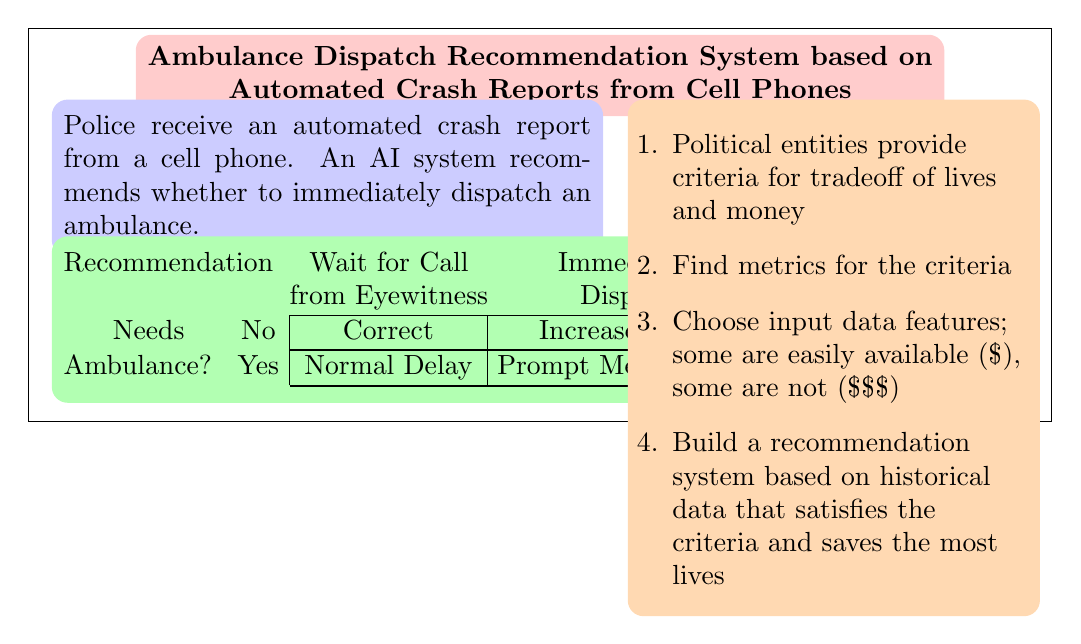
\begin{tikzpicture}[x=10mm, y=10mm, node distance = 3mm]
%	\clip (0,0) rectangle (13,5);

	\draw (0,0) rectangle (13,5);
	
	\node (Title) at (6.5,4.4) [
		align=center, 
		fill=red!20, 
		inner sep = 1.5mm,
		rounded corners=2mm
	] {  
	\bf Ambulance Dispatch Recommendation System based on \\   
	\bf Automated Crash Reports from Cell Phones
	};
	
	\node (A) at (3.8,3.1) [
		fill=blue!20, 
		inner sep = 1.5 mm, 
		rounded corners=2mm
	] {
		\begin{tabular}{@{}p{6.7cm}@{}}
			Police receive an automated crash report from a cell phone.  
			An AI system recommends whether to immediately dispatch an ambulance.
			%Should they immediately dispatch an ambulance?
		\end{tabular}
	};
	
	\node [
		below  = 1.8cm of A.west, 
		anchor=west, 
		fill=green!30,
		inner sep = 1.5mm,
		rounded corners=2mm
	] (B) {
		\begin{tabular}{@{} c @{} c @{\hspace{2pt}} | @{} c @{} | @{} c @{} | @{}c}
		\multicolumn{2}{@{}l}{Recommendation} & \multicolumn{1}{ @{} c @{} }{Wait for Call} & \multicolumn{1}{ @{} c @{} }{Immediately}   \cr
		&\multicolumn{1}{ @{} c @{} }{} & \multicolumn{1}{ @{} c @{} }{from Eyewitness} & \multicolumn{1}{ @{} c @{} }{Dispatch} \cr\cline{3-4}
		Needs & No & Correct & Increased Cost
			\vrule width 0pt height 9pt depth 2pt \cr\cline{3-4}
		Ambulance? \ \ &Yes & 
			Normal Delay & \ Prompt Medical Help \
			\vrule width 0pt height 9pt depth 4pt \cr\cline{3-4}
			\noalign{\vskip 2pt}
		\end{tabular}
		
	};

	\node (C) [
		right = 3mm of A.north east, 
		anchor = north west, 
		text width = 5cm, 
		fill=orange!30,
		rounded corners=2mm
	] {
		\vspace{-\topsep}
		\vspace{4pt}
		\begin{enumerate}[leftmargin=*]
			\item Political entities provide criteria for tradeoff of lives and money
			\item Find metrics for the criteria 
			\item Choose input data features; some are easily available (\$), some are not (\$\$\$)
			\item Build a recommendation system based on historical data that satisfies the criteria and saves the most lives
		\end{enumerate}
		\vspace{4pt}
	};

\end{tikzpicture}
}


\end{graphicalabstract}

% Research highlights
\begin{highlights}
	\item  Supports transferability and benchmarking of different approaches on a public large-scale dataset.  We have made public (on GitHub) the code we used to perform the analysis on data from the Crash Report Sampling System (CRSS) and all of the output data.  
	\item Novel Application motivated by Emerging Technology:  Machine learning classification models for dispatching ambulances based on automated crash reports from cell phones.  
	\item New Use of Dataset:  We used the Crash Report Sampling System (CRSS), which has imputed missing values for some features, but not for all of the features we wanted to use.  For the first time we have seen, we used the software the CRSS authors use for multiple imputation (IVEware) to impute missing values in more features, then compared the results with other imputation methods.
	\item Explicit Incorporation of Imbalanced Costs:  False Positives give additional cost, False Negatives give delayed medical care.
	\item Explicit Incorporation of Political Dimensions: Framing the decision threshold as a government budget question.
	\item Consideration of Marginal Effects of Threshold Shifting
	\item Perennial Machine Learning Challenge:  Imbalanced Datasets
\end{highlights}

% Keywords
% Each keyword is seperated by \sep
\begin{keywords}
 \sep Automated crash notification 
 \sep Ambulance dispatch 
 \sep Emergency medical services  
 \sep Machine learning 
 \sep Imbalanced Cost 
 \sep Imbalanced Data 
 \sep Imputation
\end{keywords}

\maketitle

% Main text

%%%%%
%
% To Do
%
%
%%%%%

%\tableofcontents
%\listoffigures
%\listoftables

%%%%% Introduction
% Introduction
\section{Introduction}
\label{intro}

\subsection{Overview}
\label{intro_overview}

[Write overview]

To train the models we would wish to have actual data on crashes with automated crash reports from cell phones, but no large public dataset exists.  As a proxy, we used the 2016-2021 data from the Crash Report Sampling System.  In \S \ref{dataset} we describe the dataset and how we binned features and imputed missing data.  

We will also consider the cost of the data inputs.  The emergency dispatcher has some information before the notification comes in, like day of week, time of day, and weather.  Some data features would require significant budgets to obtain and maintain.  There are other features useful in predicting whether the crash person needs an ambulance that, to have the data instantaneously available to emergency dispatchers might pose privacy and data security concerns.  We will call these three categories of data features Easy, Medium, and Hard, but could also describe them as Free, Expensive, and Problematic.  We discuss the data features in \S \ref{features}.

We used eight supervised learning algorithms, some with class weights and focal loss, to give 13 different models.   (See \S \ref{models}) For each of the three political criteria we find the best model based on how many ambulances it correctly recommends for immediate dispatch within the limits of the criterion.  We do this for the three sets of data features to show whether increasing the budget for data acquisition improves the system sufficiently to justify the cost, understanding that ``sufficiently'' is a political, not technical, decision.  



\subsection{Scenario}
\label{intro_scenario}

In the (fictitious) city of Springfield, the city council and mayor are debating whether to immediately dispatch ambulances based on automated notifications from cell phones.  Many residents have cell phones (iPhones and Google Pixels) whose accelerometers will detect the deceleration profile of a crash and automatically notify the emergency call center, which immediately dispatches a police officer.  The government officials are pleased that, because of the automated notifications, the police response to the crash scene is faster.  Should they also immediately dispatch an ambulance, making the medical response faster?

Traditionally, the emergency call center did not know about a crash until an eyewitness called, and the eyewitness could say whether the crash persons needed an ambulance, but that information does not come with an automated crash notification from a cell phone. The notification will come with a location, the emergency dispatcher already has some information (time of day, day of week, weather, urbanicity), and the cell service provider may provide some information about the primary user of the cell phone (age, sex).  With that information, the emergency dispatcher has three options.

\begin{itemize}
	\item Always immediately dispatch an ambulance, most of which will not be needed
	\item Never immediately dispatch an ambulance; instead, wait for a call from an eyewitness.  Many of the ambulances eventually sent to crashes had a cell phone notification and could have been sent sooner.  
	\item Sometimes.  Develop and implement an AI recommendation system to decide which to send immediately, reserving the option to send an ambulance later based on a call from an eyewitness.  
\end{itemize}


In Springfield today, without immediate ambulance dispatch based on automated crash notifications from cell phones, 50\% of dispatched ambulances go to automobile crashes and 10\% of crash persons need an ambulance.  Twenty percent of the crashes first have an automated notification from a cell phone, then a call from an eyewitness telling whether or not the crash person needs an ambulance.  The other 80\% of crashes only have an eyewitness call.  Of the crashes with automated notifications from cell phones, 15\% will need an ambulance, 
%($\text{P} = \text{FN} + \text{TP}$), 
and 85\% will not. 
%($\text{N} = \text{TN} + \text{FP}$).  
In Figure \ref{intro_springfield_before} we have scaled the numbers per 100 ambulances sent before implementation of immediate ambulance dispatch.  

(We chose these numbers for clarity of explanation, and an actual implementation would use local data.  For details on the 85/15 split, see \S\ref{dataset} Dataset and \S\ref{simplifying_assumptions} Simplifying Assumptions.)

\begin{figure}[h]
	% Image 15 cm wide
% Add 0.5cm on right for margin
\noindent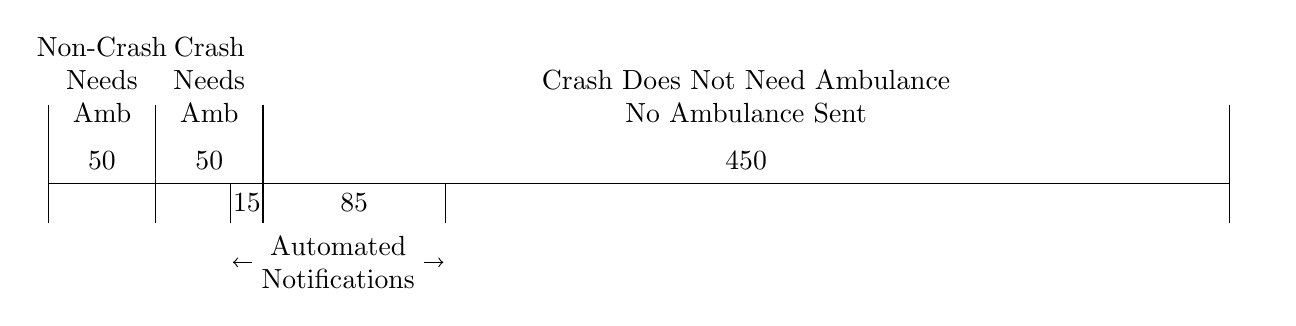
\begin{tikzpicture}[x=0.02727cm, y=0.5cm, font=\normalfont\normalsize]
	\path (568,0) circle (0pt); % Add 0.5 cm on right for margin
	\draw [color=black] (0,0) -- (550,0);
	\draw [color=black] (0,2) -- (0,-1);
	\draw [color=black] (50,2) -- (50,-1);
	\draw [color=black] (100,2) -- (100,-1);
	\draw [color=black] (550,2) -- (550,-1);
	\node (A) at (25,0) {};
	\node (B) [above=-2pt of A, align=center, text=black] {
		Non-Crash \\ Needs \\ Amb \\[0.5em] 50
	};
	\node (C) at (75,0) {};
	\node (D) [above=-2pt of C, align=center, text=black] {
		Crash \\ Needs \\ Amb \\[0.5em] 50
	};
	\node (E) at (325,0) {};
	\node (F) [above=-2pt of E, align=center, text=black] {
		Crash Does Not Need Ambulance \\ No Ambulance Sent \\[0.5em]  450
	};
	\draw [color=black] (85,0) -- (85,-1);
	\draw [color=black] (185,0) -- (185,-1);
	\path (85,0) -- (100,0) node [below, midway, color=black] {
		15
		};
	\path (100,0) -- (185,0) node [below, midway, color=black] {
		85
	};
	
	\draw [<->, color=black]  (86,-2) -- (184,-2) 
		node [midway, color=black, fill=white, align=center] 
		{Automated \\ Notifications};
%	
%	\path (85,-1) -- (185,-1) node 
%		[below, midway, color=black, align=center] {
%		Automated \\ Notifications
%	};
\end{tikzpicture}

\caption{\normalfont\normalsize Springfield before implementing immediate dispatch of ambulances.  Figure accompanies \S\ref{intro_scenario}}
\label{intro_springfield_before}
\end{figure}

\FloatBarrier

If Springfield were to implement an AI recommendation system to immediately dispatch ambulances based on automated calls from cell phones, the recommendations would not perfectly predict which crash persons need an ambulance.    See Figure \ref{intro_springfield_after}, where we have zoomed in on the left side of Figure \ref{intro_springfield_before}. In our per-100-ambulances-currently-sent proportions, the recommendation system would classify each of the automated notifications as needing or not needing an ambulance.  

Of the fifteen automated crash notifications that need an ambulance, the system would correctly classify some of them as needing an ambulance (True Positives, TP), and those crash persons would get medical attention more promptly, which is the goal and benefit of the recommendation system.  The rest of those fifteen would be incorrectly classified as probably not needing an ambulance with a recommendation to wait for a call from an eyewitness before sending one. (False Negatives, FN).  Note that the false negatives get an ambulance just as quickly under the new system as under the old,  with an ambulance dispatched upon call from an eyewitness.  

Of the 85 automated notifications that do need an ambulance, some would be correctly classified (True Negatives, TN), but some would be incorrectly classified and we would immediately dispatch an unneeded ambulance (False Positives, FP).  Besides administration, those additional ambulance runs are the cost of immediately dispatching ambulances.  In the short term those additional ambulance runs could be more than current resources (ambulances and their teams) could handle, and in the long term could be unnacceptably expensive.  

\begin{figure}[h]
	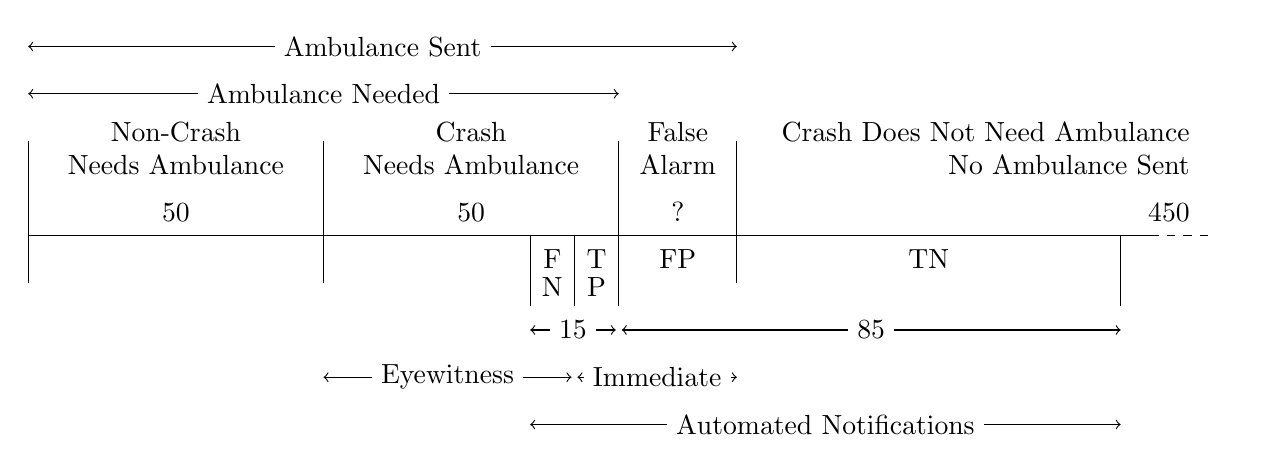
\begin{tikzpicture}[x=0.075cm, y=0.6cm, font=\normalfont\normalsize] % 15 cm wide
	\path (207,0) circle (0pt);
	\draw [color=black] (0,0) -- (190,0);
	\draw [color=black, dashed] (190,0) -- (200,0);
	\draw [color=black] (0,2) -- (0,-1);
	\draw [color=black] (50,2) -- (50,-1);
	\draw [color=black] (100,2) -- (100,-1.5);
	\draw [color=black] (120,2) -- (120,-1);
	\node (A) at (25,0) {};
	\node (B) [above=-2pt of A, align=center, text=black] {
		Non-Crash \\ Needs Ambulance \\[0.5em] 50
	};
	\node (C) at (75,0) {};
	\node (D) [above=-2pt of C, align=center, text=black] {
		Crash \\ Needs Ambulance \\[0.5em] 50
	};
	\node (E) at (200,0) {};
	\node (F) [above left =-2pt and 0pt of E, align=right, text=black] {
		Crash Does Not Need Ambulance \\ No Ambulance Sent \\[0.5em] 450
	};
	\node (G) at (110,0) {};
	\node (H) [above=-2pt of G, align=center, text=black] {
		False \\ Alarm \\[0.5em] ?
	};

	\draw [color=black] (85,0) -- (85,-1.5);
	\draw [color=black] (185,0) -- (185,-1.5);
%	\path (85,-2) -- (100,-2) node [below, midway, color=black] {15};
%	\path (100,-1) -- (185,-1) node [below, midway, color=black] {85};
	
	\draw [<->, color=black]  (100.5,-2) -- (185,-2) 
		node [midway, color=black, fill=white, align=center] 
		{85};

	\draw [<->, color=black]  (85,-2) -- (99.5,-2) 
		node [midway, color=black, fill=white, align=center] 
		{15};

	\draw [<->, color=black]  (50,-3) -- (92,-3) 
		node [midway, color=black, fill=white, align=center] 
		{Eyewitness};

	\draw [<->, color=black]  (93,-3) -- (120,-3) 
		node [midway, color=black, fill=white, align=center] 
		{Immediate};

	\draw [<->, color=black]  (85,-4) -- (185,-4) 
		node [midway, color=black, fill=white, align=center] 
		{Automated Notifications};

	\draw [<->, color=black]  (0,3) -- (100,3) 
		node [midway, color=black, fill=white, align=center] 
		{Ambulance Needed};

	\draw [<->, color=black]  (0,4) -- (120,4) 
		node [midway, color=black, fill=white, align=center] 
		{Ambulance Sent};

%	\node (G) at (110,2) [color=black, align=left] {False \\  Alarm};
	\path (100,-0.5) -- (120,-0.5) node [midway, color=black] {FP};
	\path (120,-0.5) -- (185,-0.5) node [midway, color=black] {TN};
	\draw [color=black] (92.5,0) -- (92.5,-1.5);
	\path (85,-0.5) -- (92.5,-0.5) node [midway, color=black] {F};
	\path (85,-1.2) -- (92.5,-1.0) node [midway, color=black] {N};
	\path (100,-0.5) -- (92.5,-0.5) node [midway, color=black] {T};
	\path (100,-1.2) -- (92.5,-1.0) node [midway, color=black] {P};
\end{tikzpicture}

\caption{\normalfont\normalsize Springfield after implementing immediate dispatch of ambulances.  Figure accompanies \S\ref{intro_scenario}}
\label{intro_springfield_after}
\end{figure}

\FloatBarrier

The leaders of Springfield need to find a balance between the benefit of more prompt medical attention and the cost of sending more ambulances.  The tradeoff of lives and money is not ethically or morally comfortable, but that is the choice governments make when they set budgets for health care and emergency services.  In the confusion matrices in Figure \ref{intro_confusion}, Springfield would love to increase TP without increasing FP, but the recommendation system will not give perfect predictions.  

\begin{figure}[h]
\begin{minipage}{\linewidth}
{\normalfont\normalsize
\begin{tabular}{p{2in}p{3in}}
\begin{tabular}{c c  | c | c | c}
	& \multicolumn{1}{c}{} & \multicolumn{2}{c}{Prediction}  \cr
	&\multicolumn{1}{c}{} & \multicolumn{1}{c}{PN} & \multicolumn{1}{c}{PP} \cr\cline{3-4}
	\multirow{2}{*}{Actual} & N & TN & FP \vrule width 0pt height 10pt depth 2pt \cr\cline{3-4}
	 & P & FN & TP	\vrule width 0pt height 10pt depth 4pt \cr\cline{3-4}
\end{tabular}
&
\begin{tabular}{c c  | c | c | c}
	\multicolumn{2}{@{}l}{Recommendation} & \multicolumn{1}{ @{} c @{} }{Wait for Call} & \multicolumn{1}{ @{} c @{} }{Immediately}   \cr
	&\multicolumn{1}{ @{} c @{} }{} & \multicolumn{1}{ @{} c @{} }{from Eyewitness} & \multicolumn{1}{ @{} c @{} }{Dispatch} \cr\cline{3-4}
	Needs & No & Correct & Increased Cost
		\vrule width 0pt height 10pt depth 2pt \cr\cline{3-4}
	Ambulance? \ \ &Yes & 
		Normal Delay & \ Prompt Medical Help \
		\vrule width 0pt height 10pt depth 4pt \cr\cline{3-4}
\end{tabular}
\cr		
\end{tabular}
}
\end{minipage}
\caption{\normalfont\normalsize Confusion matrix for ambulance dispatch.  Figure accompanies \S\ref{intro_scenario}}
\label{intro_confusion}
\end{figure}

\FloatBarrier

Building Springfield's AI recommendation system starts with an historical dataset with the features the emergency dispatchers will have at the time of the automated notification, like time of day, weather, maybe age and sex, and possibly more information, and whether that historical crash person needed an ambulance (supervised learning).  A machine learning algorithm learns a model of the data, and when an automated crash notification comes in, given the data available, the model returns a value $p \in [0,1]$ that increases with the probability that the crash person needs an ambulance.  Choosing $p=1$ would mean never immediately dispatching an ambulance, and $p=0$ would be always.  The city council and mayor need to choose a decision threshold $\theta$ such that if, for a particular crash notification, $p>\theta$, then immediately dispatch an ambulance; if $p<\theta$, wait for a call from an eyewitness.  

The histogram in Figure \ref{intro_ideal} shows typical model output.  The model generally gives lower $p$ values to crash persons who do not need an ambulance (Neg) and higher $p$ values to crash persons who do need an ambulance (Pos), but there is significant overlap.  The most obvious feature of the histogram is the class imbalance, that there are many more Neg than Pos, in fact $85/15 \approx 6$ Neg for each Pos.  

  Given a choice of $\theta$, Springfield would immediately dispatch ambulances to all of the crashes to the right of $\theta$.  The Pos (Needs ambulance) to the right of $\theta$ (TP) would get more prompt medical attention, but the Neg (Does not need ambulance) to the right (FP) would be wasted ambulance runs.  At $\theta = 0.8$, TP and FP are about equal, but as we consider smaller $\theta$ the number of TP increases by smaller and smaller amounts while the number of FP grows dramatically.  

\begin{figure}[h]
\centering
	\input{../Keras/Images/Ideal_Pred_Wide.pgf}	
\caption{\normalfont\normalsize Example model test results.  Figure accompanies \S\ref{intro_scenario}}
\label{intro_ideal}
\end{figure}

\FloatBarrier

We will consider three ways the leaders of Springfield can think about how to choose $\theta$, three metrics for political decision thresholds, detailed in \S \ref{political_decisions}.

\begin{enumerate}
	\item Percent increase in number of ambulance calls
	\item Percent of immediately dispatched ambulances that are actually needed
	\item Minimum probability that an immediately dispatched ambulance is actually needed
\end{enumerate}











%%%%% Methods
\section{Methods}\label{sec:Methods}

%%%% Methods

\subsection{Outline}

\begin{enumerate}
	\item Political Goals
	\item Metrics for Political Goals
	\item The Dataset
	\item Choosing Features
	\item Building Models
	\item Analysis of Cost/Benefit
	\item Choosing the Best Model
\end{enumerate}
\begin{figure}[h]
\centering
\normalfont\normalsize



\tikzstyle{startstop} = [
	rectangle, rounded corners, 
	%minimum width=3cm, 
	%minimum height=1cm,
	text centered, 
	draw=black, 
	fill=red!20,
	text=black
]

\tikzstyle{io} = [
	trapezium, 
	trapezium stretches=true, % A later addition
	trapezium left angle=70, 
	trapezium right angle=110, 
	%minimum width=3cm, 
	%minimum height=1cm, 
	text centered, 
	draw=black, 
	fill=blue!20,
	text=black
]

\tikzstyle{process} = [
	rectangle, 
	%minimum width=3cm, 
	%minimum height=1cm, 
	text centered, 
	%text width=3cm, 
	draw=black, 
	fill=orange!30,
	text=black
]

\tikzstyle{decision} = [
	diamond, 
	%minimum width=3cm, 
	%minimum height=1cm, 
	text centered, 
	aspect=5,
	draw=black, 
	fill=green!30,
	text=black
]

\tikzstyle{arrow} = [thick,->,>=stealth]

\begin{tikzpicture}[x=10mm, y=10mm, node distance = 4mm]
	\clip (0,0) rectangle (13,5);
%	\draw (0,0) rectangle (13,5);
	
%	\node (Title) at (6.5,4.4) [align=center] { \bf Ambulance Dispatch Recommendation System based on \\  \bf Automated Crash Reports from Cell Phones};
	\node [text=black] (Title) at (6.5,4.6) [align=center] { \bf Methods};

	\node (A) at (3.3,3.9) [startstop] {Criteria (Given by Politicial Process)};
	
	\node (B) [process, below= of A] (B) {Metrics for Budgetary Criteria};
	\node [decision, below= of B, align=center] (C) {Choose Data};

	\draw [arrow] (A) -- (B);
	\draw [arrow] (B) -- (C);

	\node [io, below = of C] (E) {\$\$};
	\node [io, left= of E] (D) { \ \ \$ \ \ };
	\node [io, right= of E] (F) {\$\$\$};

	\draw [arrow] (C.south west) -- (D);
	\draw [arrow] (C.south) -- (E);
	\draw [arrow] (C.south east) -- (F);

	\node [process, right = 2 cm of A] (G) {Build Multiple ML Models};

	\draw [arrow] (D.south)  |- ++(0,-0.3) -- ++(4.5,0)  |- (G);
	\draw [thick] (E.south) -- ++(0,-0.3);
	\draw [thick] (F.south) -- ++(0,-0.3);

	\node [io, below= of G] (H) {Marginal and Total Results};

	\node [process, below = of H] (J) {Analysis of Costs/Benefits};

	\node [startstop, below=of J, align=center] (K) {Deliver Options to \\ Political Decision Makers};

	\draw [arrow] (G) -- (H);
	\draw [arrow] (H) -- (J);
	\draw [arrow] (J) -- (K);
\end{tikzpicture}

\caption{\normalfont\normalsize Methods Graphical Abstract}
\label{methods_graphical_abstract}
\end{figure}

\FloatBarrier
% Political Decisions
\subsection{Budgetary Decision Thresholds and Corresponding Metrics}
\label{political_decisions}

Saying that we trade off lives for money makes us uncomfortable, but that is what governments do when they set budgets for health care and emergency services.  All budgets are finite, and spending more money has diminishing returns, so we have to choose some criteria for our decision and accompanying metrics that let us quantify the criteria to choose an appropriate decision boundary for our recommendation system.  

Our Springfield scenario illustrates the tradeoffs.  We consider three ways to set the decision threshold.  

\begin{figure}[h]
	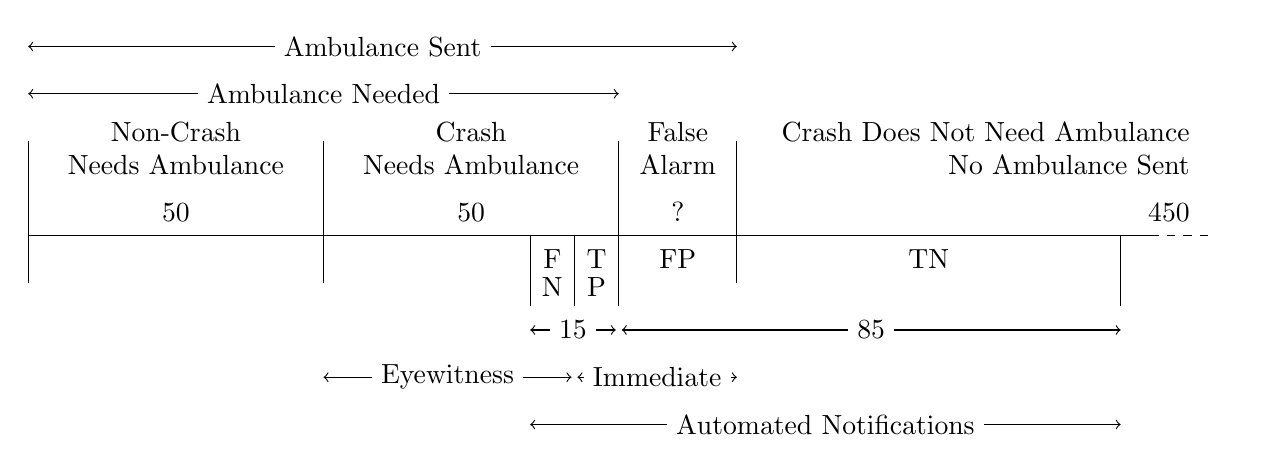
\begin{tikzpicture}[x=0.075cm, y=0.6cm, font=\normalfont\normalsize] % 15 cm wide
	\path (207,0) circle (0pt);
	\draw [color=black] (0,0) -- (190,0);
	\draw [color=black, dashed] (190,0) -- (200,0);
	\draw [color=black] (0,2) -- (0,-1);
	\draw [color=black] (50,2) -- (50,-1);
	\draw [color=black] (100,2) -- (100,-1.5);
	\draw [color=black] (120,2) -- (120,-1);
	\node (A) at (25,0) {};
	\node (B) [above=-2pt of A, align=center, text=black] {
		Non-Crash \\ Needs Ambulance \\[0.5em] 50
	};
	\node (C) at (75,0) {};
	\node (D) [above=-2pt of C, align=center, text=black] {
		Crash \\ Needs Ambulance \\[0.5em] 50
	};
	\node (E) at (200,0) {};
	\node (F) [above left =-2pt and 0pt of E, align=right, text=black] {
		Crash Does Not Need Ambulance \\ No Ambulance Sent \\[0.5em] 450
	};
	\node (G) at (110,0) {};
	\node (H) [above=-2pt of G, align=center, text=black] {
		False \\ Alarm \\[0.5em] ?
	};

	\draw [color=black] (85,0) -- (85,-1.5);
	\draw [color=black] (185,0) -- (185,-1.5);
%	\path (85,-2) -- (100,-2) node [below, midway, color=black] {15};
%	\path (100,-1) -- (185,-1) node [below, midway, color=black] {85};
	
	\draw [<->, color=black]  (100.5,-2) -- (185,-2) 
		node [midway, color=black, fill=white, align=center] 
		{85};

	\draw [<->, color=black]  (85,-2) -- (99.5,-2) 
		node [midway, color=black, fill=white, align=center] 
		{15};

	\draw [<->, color=black]  (50,-3) -- (92,-3) 
		node [midway, color=black, fill=white, align=center] 
		{Eyewitness};

	\draw [<->, color=black]  (93,-3) -- (120,-3) 
		node [midway, color=black, fill=white, align=center] 
		{Immediate};

	\draw [<->, color=black]  (85,-4) -- (185,-4) 
		node [midway, color=black, fill=white, align=center] 
		{Automated Notifications};

	\draw [<->, color=black]  (0,3) -- (100,3) 
		node [midway, color=black, fill=white, align=center] 
		{Ambulance Needed};

	\draw [<->, color=black]  (0,4) -- (120,4) 
		node [midway, color=black, fill=white, align=center] 
		{Ambulance Sent};

%	\node (G) at (110,2) [color=black, align=left] {False \\  Alarm};
	\path (100,-0.5) -- (120,-0.5) node [midway, color=black] {FP};
	\path (120,-0.5) -- (185,-0.5) node [midway, color=black] {TN};
	\draw [color=black] (92.5,0) -- (92.5,-1.5);
	\path (85,-0.5) -- (92.5,-0.5) node [midway, color=black] {F};
	\path (85,-1.2) -- (92.5,-1.0) node [midway, color=black] {N};
	\path (100,-0.5) -- (92.5,-0.5) node [midway, color=black] {T};
	\path (100,-1.2) -- (92.5,-1.0) node [midway, color=black] {P};
\end{tikzpicture}

\caption{\normalfont\normalsize Springfield after implementing immediate dispatch of ambulances.  Figure accompanies \S\ref{intro_scenario}}
\label{methods_springfield_after}
\end{figure}

\FloatBarrier




%%%%%
\subsubsection{Budgetary Decision Metric I:  Percent Increased Number of Ambulance Calls}
\label{political_decisions_percent_increased}

When a city or region implements immediate dispatch of ambulances, the number of ambulance dispatches increases by FP.   Within the automated notifications, 
$\text{P} = \text{FN} + \text{TP}$
 ambulance runs becomes P + FP = FN + TP + FP ambulance runs, an increase by a rate of $\text{FP}/\text{P}$.  The increase does not include the true positives (TP), because those ambulances would go eventually with or without immediate dispatch; the increase is the number of false positives (FP).  
 
In the short term (too short to buy more ambulances and hire more teams), the existing budget can support an increase in the number of ambulance runs to crash persons by some small percentage.  In the longer term, the city is willing to increase the budget to increase the number of ambulances going to crashes with automated notifications by a larger, but still fixed, percentage.  We use 5\% as our example of how to implement this policy, setting the decision threshold $\theta$ where the number of false positives is 5\% of the positive class, giving our first budgetary decision metric,

\begin{equation} \label{eq:budget_1}\hfil
\frac{ \text{FP}}{\text{P}}
=
\frac{ \text{FP}}{\text{FN} + \text{TP}}
\le 0.05
\end{equation}

 In our Springfield scenario, scaling to 100 currently sent ambulances to crash or non-crash, the total number of ambulance runs goes from 100 to 100 + FP, a rate of increase of $\text{FP}/100$.  For any city or region, if we knew the proportion of crashes with automated notifications from cell phones and the proportion of ambulances going to crashes, we could choose an
 $\text{FP}/\text{P}$
 threshold to match a budgetary decision criterion based on the increase in total number of ambulances sent to crashes or total number of ambulances sent to any situation.


%%%%%
\subsubsection{Budgetary Decision Metric II:  Percent of Immediately Dispatched Ambulances Actually Needed}
\label{political_decisions_precision}

A city or region is willing to immediately dispatch ambulances based on automated crash reports, but only up to the point where a certain proportion of the ambulances they immediately dispatch 
$(\text{PP} = \text{FP} + \text{TP})$ 
are actually needed (TP).  This proportion, 
$\text{TP}/(\text{FP} + \text{TP})$ 
is called the {\it precision} of a machine learning model.  In this paper we use the term {\it precision} in this sense and {\it numerical precision} to describe the confidence we can have in a certain number of decimal places of a result.

To illustrate the method, we choose $\text{Precision} = 2/3$, being willing to immediately dispatch one unnecessary ambulance for each two necessary ones, giving our second budgetary decision metric,

\begin{equation} \label{eq:budget_2}\hfil
\frac{ \text{TP}}{\text{PP}}
=
\frac{ \text{TP}}{\text{FP} + \text{TP}}
\ge \frac{2}{3}
\end{equation}

%%%%%
\subsubsection{Budgetary Decision Metric III:  Minimum Probability that Each Immediately Dispatched Ambulance is Needed}
\label{political_decisions_probability}

The previous two decision criteria let the city leaders choose a specific dollar amount of increase in the annual ambulance budget, but for ethical reasons they may decide that, while they cannot afford to immediately dispatch an ambulance to every crash notification, they should immediately dispatch an ambulance to a crash notification with some probability (like 50\% or 80\%) of needing medical attention, and consider the total cost later.  From our model results, can we find a decision threshold $\theta$ that corresponds to such a probability?

Our recommendation system uses a supervised-learning binary classification model trained on historical data. The models do not actually return a probability but return, for each sample, a value $p$ that generally increases with the probability.  For each sample we also know whether that historical crash person actually needed an ambulance (whether that sample is in the negative or positive class).  

Consider a small band of values of $p$; the samples in that band are either in the negative or positive class.  Call the number of negative and positive samples in the band Neg and Pos, to distinguish from the total number of samples in the negative and positive classes, N and P.  The probability that a crash person in that band of $p$ needs an ambulance is given by 
$\text{Pos}/(\text{Neg} + \text{Pos})$, which we call ``marginal probability,'' or ``$m$Prob.''

To illustrate the method, we choose the minimum marginal probability to be 50\%, meaning that each ambulance we immediately dispatch has at least a fifty percent chance of being needed, giving our third budgetary decision metric,

\begin{equation} \label{eq:budget_3}\hfil
m\text{Prob} =  \frac{\text{Pos}}{\text{Neg}+\text{Pos}} \ge 0.5
\end{equation}


We can relate this metric to a familiar metric if we rephrase the probability as the ratio of needed to unneeded ambulances immediately dispatched, {\it i.e.} Pos:Neg.  For instance, a 50\% probability is a 1:1 ratio of needed to unneeded, and an 80\% probability is a 4:1 ratio of needed to unneeded.  
The proportion of needed to unneeded ambulances sent in a neighborhood of $p$ is proportional to a widely used metric, the slope of the ROC curve, with the constant of proportionality being the class ratio, as shown here:  

\begin{equation} \label{eq:ROC_slope}\hfil
\frac{\text{Pos}}{\text{Neg}}
=\frac{\Delta\text{TP}}{\Delta \text{FP}}
=\frac{\text{P}}{\text{N}} \cdot \frac{\Delta\text{TP}/\text{P}}{\Delta \text{FP}/\text{N}} 
=\frac{\text{P}}{\text{N}} \cdot \frac{\Delta\text{TPR}}{\Delta \text{FPR}}
=\frac{\text{P}}{\text{N}} \cdot m\text{ROC}
\end{equation}


\subsection{Dataset}
\label{dataset}

Ideally, we would use a dataset of crashes that spawned an automated notification, but we have not found such a dataset that is publicly available.  Working with such a private dataset would be an important avenue of future research. (See \S \ref{simplifying_assumptions} for a list of simplifying assumptions and opportunities for future research.)

We will use the Crash Report Sampling System (CRSS) data from 2016 to 2021.  The CRSS is a curated sample of crashes in the US, weighted to more serious crashes such that 17\% of the crash persons needed an ambulance, significantly more than the proportion of all reported crashes needing an ambulance.  Since many low-speed crashes would have a crash profile similar to hard braking, they would not spawn an automated notification, so it is reasonable to assume that the set of crashes with automated notifications would have a higher percentage of persons needing an ambulance.  

We make some simplifying assumptions (see \S\ref{simplifying_assumptions}) using this dataset, including that the class ratio (N:P) in the automated crash notification from cell phones will be close to that in the CRSS data, 5:1, and that the crash persons in the CRSS data are representative of the future crash persons whose cell phones send a crash notification.  We will use the CRSS as a proxy for the set of crashes with automatic crash notifications, acknowledging that we do not know how good of a proxy it is. The primary merit of CRSS for our work is that it is publicly available so that our work can be critiqued, adapted, and expanded by others.  

To prepare the data we had to bin (discretize) some features and to impute missing data.  Some features in CRSS have both the original data with values signifying ``Missing'' or ``Unknown'' and a new feature with missing values imputed using IVEware \citep{IVEware}, but not all of the features we wanted to use had imputed values.  CRSS has a very useful document on the history of its imputation methods going back to 1988 with the predecessors of the current data set \citep{CRSS_Imputation}.  We debated the proper order of operations for binning and imputing, tried both, and decided to bin first, then impute.  We tried several methods of imputation, including the IVEware used by the CRSS authors, but got better results using a round-robin random forest method.  Full details and analysis are in the code, listed below.

We removed all crashes involving a pedestrian because deceleration profile of such a crash would be more like hard braking than hitting a large immovable object like a car or tree, so less likely to trigger an automated notification.  

The dataset is slightly imbalanced, with five elements of the negative class for each element of the positive class.  We considered several methods to handle the imbalance, including resampling, class weights, focal loss \citep{lin2017focal}, and balanced metrics.  We cannot use the popular SMOTE oversampling method because our data is categorical \citep{Chawla_2002}.  We tried undersampling with Tomek Links, but the resulting model results were not significantly different.  The best results came from using the model algorithms from Imbalanced-Learn \citep{Imblearn}, some of which apply bagging on top of algorithms from Scikit-Learn \citep{scikit-learn}.

After removing those pedestrian crashes we had 713,566 samples, each representing a crash person, and 78 relevant features.  For details, see these sections of code in the {\tt Keras} folder at 

\url{www.github.com/bburkman/Ambulance_Dispatch}.

\

\begin{tabular}{l}
	\verb|Ambulance_Dispatch_01_Get_Data.ipynb| \cr
	\verb|Ambulance_Dispatch_02_Correlation.ipynb| \cr
	\verb|Ambulance_Dispatch_03_Bin_Data.ipynb| \cr
	\verb|Ambulance_Dispatch_04_Impute_Missing_Data.ipynb| \cr
	\verb|Ambulance_Dispatch_05_IVEware_Order_of_Operations.ipynb| \cr
	\verb|Ambulance_Dispatch_06_Build_Models_Tomek_Links.ipynb| \cr
\end{tabular}



\subsection{Choosing Features}
\label{features}

The \verb|Accident|, \verb|Vehicle|, and \verb|Person| files of the CRSS dataset 2016-2021 have 170 unique features.  

First we want to narrow the features to those that are relevant, of good quality, and knowable at the at the time of the automated notification (before any eyewitness reports).  Some features, like Vehicle Identification Number (VIN), have no predictive value.  Other features have missing data for more than 20\% of samples.  Some features, like drug and alcohol test results, are unknowable at the time of the automated notification.

Having data available for instantaneous analysis when the crash notification comes in is not free, and some features are more expensive than others.  A city thinking of implementing a recommendation system for immediate dispatch will need to decide how much to spend to have the data available, and whether the more expensive features increase the quality of the models enough to be worth the cost.  We categorized the features as ``Easy,'' ``Medium,'' and ``Hard,'' which can also be called ``Free,'' ``Expensive,'' and ``Problematic.''   The ``Easy'' features are those the dispatcher already has, like day of week, time of day, weather, and urban/rural.  The ``Medium'' features add details about the location (intersection, speed limit, interstate highway) and information the cell service company probably has about the primary user of the phone (age and sex).  To have the medium features instantaneously available would require coordination of many resources and be expensive to set up.  The ``Hard'' features are much more problematic, requiring more coordination of public and private records, and introduce privacy and data security issues.  Hard features include whether the location is a work zone, the likely vehicle driven by the primary user of the cell phone, and, if there are multiple automated notifications from the same location, how many crash persons are likely to be involved.   

We note here our simplifying assumption (\S \ref{simplifying_assumptions}) that we will have complete and accurate data for each automated notification.  Also, we will test three combinations of features but have not done more detailed testing to see which individual features or groups of features are most or least useful in predicting whether a crash person needs an ambulance.  

See 
\verb|Ambulance_Dispatch_01_Get_Data.ipynb|  
for a list of the excluded features.

See \verb|Ambulance_Dispatch_03_Bin_Data.ipynb|
for a list of the features we used for imputation of missing data in CRSS.


See
\verb|Ambulance_Dispatch_07_Build_Models.ipynb|.
for the complete list of the features used in the Easy, Medium, and Hard model building.
\subsection{Models}
\label{models}

See \verb|Ambulance_Dispatch_07_Build_Models.ipynb| for more details.  

%%%%%
\FloatBarrier
\subsubsection{Binary Classification Algorithms and Hyperparameters}
\label{algorithms}

For each of the three sets of features we used eight binary classification algorithms, three of which take class weight $\alpha$ and one of which takes the focal loss parameter $\gamma$.  (See Table \ref{models}) We learned models for various values of the hyperparameters, giving $3 \times 13 = 39$ different models.  The $\alpha=0.5$ class weight is the default, and the $\alpha = 0.85$ class weight balances the effect of the negative and positive class in the loss function, as 85\% of the samples are in the negative class.  Focal loss \citep{lin2017focal} puts more weight in the loss function on the samples that are badly classified, much like least squares regression puts more weight on the points furthest from the line.  Setting $\gamma=0.0$ has no effect; Lin's paper tested from $\gamma=0.5$ to $\gamma = 5.0$ and recommended $\gamma = 2.0$.  

\

\begin{table}[h]
\label{models}
\caption{\normalsize\normalfont Models Tested for Recommendation System.  Table accompanies \S \ref{algorithms}}
\centering
\normalsize\normalfont
\begin{tabular}{lllcc}
&&& \bf Class &\bf Focal  \cr
\bf Model & \bf Abbreviation&\bf Source &\bf Weight $\alpha$ &\bf Loss $\gamma$ \cr\hline

AdaBoost  Classifier & AdaBoost & Scikit-Learn &  \cr\hline

Balanced Bagging Classifier & Bal Bag & Imbalanced-Learn &  \cr\hline

Balanced Random Forest Classifier & Bal RF & Imbalanced-Learn & 0.5 \cr
	&&& 0.85 \cr\hline

Easy Ensemble Classifier with AdaBoost Estimator & Easy Ens & Imbalanced-Learn &  \cr\hline

KerasClassifier with the  & Keras & Keras & 0.5 & 0.0 \cr
\qquad Binary Focal Crossentropy loss function &&& 0.5 & 1.0  \cr
	&&& 0.5 & 2.0 \cr
	&&& 0.85 & 0.0 \cr\hline

Logistic Regression Classifier & Log Reg & Scikit-Learn & 0.5 \cr
	&&& 0.85 \cr\hline

Random Forest Classifier & RF & Scikit-Learn &  \cr\hline

RUSBoost Classifier & RUSBoost & Imbalanced-Learn &  \cr

\end{tabular}
\end{table}

\FloatBarrier

\subsubsection{Hyperparameter Effects}
\label{hyperparameters}

Our experience with varying the class weight and focal loss parameters was that they shifted the entire $p$ distribution, both the positive and negative class, but did not do a better job of separating the positive and negative class, as measured by the area under the curve (AUC) of the receiver operating characteristic (ROC), as illustrated in Figure \ref{hyperparameters_figure} below.  

The KerasClassifier with the Binary Focal Crossentropy loss function takes both a class weight hyperparameter $\alpha$ and a focal loss parameter $\gamma$.  Varying these hyperparameters gave us different shapes of distributions of $p$, as shown in Figure \ref{hyperparameters_figure}, which also gives the ROC AUC for two runs of each model with different random seeds.  That the model on the left has both the least and the greatest ROC AUC illustrates that, between models of the same algorithm with different class and focal weights, the effectiveness of the model in separating the positive and negative classes depends as much on the random seed as on the choice of weights.  

If one is using the default decision threshold $\theta = 0.5$, then these hyperparameters are useful for shifting the distribution to meet the threshold, but since we are taking the liberty to move the threshold, varying the hyperparameters may be of little use.  Since the ROC AUC quantifies how well the algorithm separates the positive and negative classes over the whole range of $p$, and we are most interested in a small range of $p$ on the right end, the weights may yet have some useful effect, a topic for future investigation (\S\ref{simplifying_assumptions}).

%%%
\begin{figure}[h]
\noindent\begin{tabular}{@{\hspace{-6pt}}p{2.3in} @{\hspace{-6pt}}p{2.3in} @{\hspace{-6pt}}p{2.3in} }
	\vskip 0pt
	\hfil {\normalfont\normalsize $\alpha = 0.5$, $\gamma = 0.0$}
	\vskip 4pt
	
	{\normalfont\normalsize \ $\text{ROC AUC} \in \{ 0.777402, 0.778653 \}$ }
	
	
	\input{../Keras/Images/KBFC_alpha_0_5_gamma_0_0_Hard_Run_0_Pred.pgf}	
&
	\vskip 0pt
	\hfil {\normalfont\normalsize $\alpha = 0.5$, $\gamma = 2.0$}
	
	\vskip 4pt
	{\normalfont\normalsize \ $\text{ROC AUC} \in \{0.777903, 0.777626\}$}
		
	\input{../Keras/Images/KBFC_alpha_0_5_gamma_2_0_Hard_Run_0_Pred.pgf}	
&
	\vskip 0pt
	\hfil {\normalfont\normalsize $\alpha = 0.85$, $\gamma = 0.0$}
	
	\vskip 4pt
	{\normalfont\normalsize \ $\text{ROC AUC} \in \{0.7779, 0.778199\}$}
	
	\input{../Keras/Images/KBFC_alpha_balanced_gamma_0_0_Hard_Run_0_Pred.pgf}	
\cr
\end{tabular}
	  \caption{\normalfont\normalsize KerasClassifier with Different Hyperparameters with ROC AUC for Two Model Runs with Different Random Seeds.  Figure accompanies \S\ref{hyperparameters}}\label{hyperparameters_figure}
\end{figure}

\FloatBarrier


%%%%%
\subsubsection{Five-Fold Cross Validation}
\label{cross_validation}

As mentioned in \S\ref{political_decisions_probability}, 
we need enough samples in each band of $p$ to smooth out the randomness.  If we had more samples total, we could use smaller bands and have more numerical precision in our specification of the decision threshold $\theta$.  If we used a typical 70/30 train/test split, we would only have $p$ values for the 30\% samples in the test set.  Instead we used five-fold cross validation, having an 80/20 split five times, giving us $p$ values for all of the samples.  

%%%%%
\FloatBarrier
\subsubsection{Interpreting Supervised Learning Binary Classification Results}
\label{interpreting_ideal}

In supervised learning binary classification, a model predicts, for each sample in the test set, whether the sample is in the negative or positive class.  The model returns a value $p \in [0,1]$, that increases with the probability that the sample is in the positive class.  Additionally in supervised learning, we already know the answer to the question of whether the sample was in the negative or positive class, with $y \in \{0,1\}$ given in the dataset but hidden from the model during the test phase.  In the code, $p$ is often called \verb|y_proba| and $y$ is called \verb|y_test|.  Using these two numbers, $p$ and $y$, we can study, quantify, and illustrate how well the model predicts the actual values.  

A perfect model would entirely separate the negative and positive classes, but the ideal we can hope for is that most of the negative elements are towards the left and most of the positive elements are towards the right of the distribution.  In Figure \ref{ideal}, the data has the same class ratio as our CRSS data, with 85\% in the negative class and 15\% in the positive class.  If we choose discrimination threshold $\theta = 0.5$, the value of $p$ for which most models algorithms are optimized, the elements of the negative class with $p<\theta$ are True Negatives (TN), the elements of the negative class with $p > \theta$ are False Positives (FP), the elements of the positive class with $p < \theta$ are False Negatives (FN), and the elements of the positive class with $p > \theta$ are True Positives (TP).  

If this ideal model were our recommendation system with $\theta = 0.5$, then 38.5\% of the ambulances we immediately dispatched would be needed (Precision), and 73\% of the needed ambulances would be immediately dispatched (Recall).  If we chose a higher value of $\theta$, we would increase TN, decrease FP, increase FN, and decrease TP.  Recall would decrease, but the effect on precision is uncertain as FP and TP would both decrease.

The ROC (Receiver Operating Characteristic) curve is a parameterized curve showing the True Positive Rate (TP/P) versus the False Positive Rate (FP/N) as $p$ varies from 0 (upper right) to 1 (lower left).  The area under the curve (AUC) is widely used to compare the quality of models in terms of how well they separate the negative and positive classes over the entire range of $p \in [0,1]$.  For our work, however, given real-life budgetary constraints on expanding ambulance fleets, we are only interested in a small range of $p$ on the right side of the distribution, so the ROC AUC is not the primary measure we will use to choose the best model.

\begin{figure}[h]
\noindent\begin{tabular}{@{\hspace{-6pt}}p{2.3in} @{\hspace{-6pt}}p{2.0in} p{1.8in}}
	\vskip 0pt
	\hfil {\normalfont\normalsize Raw Model Output}
	
	\input{../Keras/Images/Ideal_Pred.pgf}	
&
	\vskip 0pt
	\hfil {\normalfont\normalsize ROC Curve}
	
	\input{../Keras/Images/Ideal_ROC.pgf}
&
	\normalfont\normalsize 
	\vskip 0pt
	Choosing decision
	
	\quad threshold $\theta = 0.5$:
	
	\
	
	\begin{tabular}{cc|c|c|}
	&\multicolumn{1}{c}{}& \multicolumn{2}{c}{Prediction} \cr
	&\multicolumn{1}{c}{} & \multicolumn{1}{c}{N} & \multicolumn{1}{c}{P} \cr\cline{3-4}
	\multirow{2}{*}{\rotatebox[origin=c]{90}{Actual}}&N &
%66.473	18.527	3.406	11.594
66.5\% & 18.5\%
	\vrule width 0pt height 10pt depth 2pt \cr\cline{3-4}
	&P & 
3.4\% & 11.6\%
	\vrule width 0pt height 10pt depth 2pt \cr\cline{3-4}
	\end{tabular}

	\hfil\begin{tabular}{ll}
	\cr
%0.384914179	0.772933333	0.51560575
0.385 & Precision \cr	0.773 & Recall \cr	%0.516 & F1 \cr
\end{tabular}

\cr
\end{tabular}
\caption{\normalfont\normalsize Example Model Results.  Figure accompanies \S\ref{interpreting_ideal}}
\label{ideal}
\end{figure}

%%%%%
\FloatBarrier
\subsubsection{Comparing Outputs of Different Models}
\label{comparing_outputs}

The eight model algorithms not only give different results, but different kinds of results, and we have to find a way to compare them.  Ideally, we will find ways to evaluate the results that will apply to all of the kinds of model output. See Figure \ref{raw_output_figure}.  For the illustrations we have used models built on the Hard features with no class balance nor focal loss.

The ranges and shapes of the distributions are significantly different.  The Balanced Bagging and  Balanced Random Forest classifiers gives a nice spread from 0.0 to 1.0, but the AdaBoost, Easy Ensemble, and RUSBoost results are clustered in the middle, and the Random Forest on the left.  If we used the Random Forest results with the default decision threshold $\theta = 0.5$, we would never immediately dispatch an ambulance.  The KerasClassifier and Logistic Regression Classifier tend towards the left with long tails to the right.  

To give appropriate results for Balanced Bagging with a $p$ range of width 1.0 and RUSBoost with a range of width 0.002, we built into the code a variable for numerical precision that depends on the range of $p$ for that model, $\text{num\_prec} = - \lceil \log_{10} ( \text{max}(p) - \text{min}(p) )  \rceil$, to which we can then add the number of digits appropriate for the purpose.  

The numerics in the model results are also different.  Most of the models give, for the 713,566 samples, at least 100,000 unique values of $p \in [0,1]$, making the discrete results nearly continuous.  The AdaBoost, KerasClassifier, Logistic Regression, and RUSBoost algorithms are fairly consistent with about 140,000 unique values of $p$ for results on the Easy features, 640,000 for the results on the Medium features, and 700,000 on the Hard features.  The Random Forest classifier gives about half as many unique results, but proportionally for the three features sets.

The outliers in the numerics are the Balanced Random Forest, Balanced Bagging, and Easy Ensemble.  The Balanced Random Forest method on the Hard features gives less than 4,000 unique values of $p$ on the Hard features because 93\% of its $p$ values are rounded to two decimal places.  The Balanced Bagging results on the Hard features have less than 300 unique values because 99\% of its $p$ values are rounded to one decimal place.  While the other algorithms had fewer unique values for the Medium features and far fewer for the Easy, the Balanced Random Forest and Balanced Bagging have more for the Medium and far more for the Easy, with the number of unique Easy results being comparable to those of the other algorithms.  The Easy Ensemble results for all three features sets have about 50\% of the results rounded to two decimal places.  For full details see \verb|Analyze_Proba/Value_Counts_y_proba.csv|.





%%% AdaBoost
\begin{figure}[h]
\noindent\begin{tabular}{@{\hspace{-6pt}}p{2.3in}@{\hspace{-6pt}}p{2.3in} @{\hspace{-6pt}}p{2.3in}}

	\vskip 0pt
	\normalfont\normalsize
	\hfil AdaBoost
	
	\input{../Keras/Images/AdaBoost_5_Fold_Hard_Test_Pred.pgf}	
&
	\vskip 0pt
	\normalfont\normalsize
	\hfil Balanced Bagging
	
	\input{../Keras/Images/BalBag_5_Fold_Hard_Test_Pred.pgf}	
&
	\vskip 0pt
	\hfil {\normalfont\normalsize Balanced Random Forest}
	
	\input{../Keras/Images/BRFC_5_Fold_alpha_0_5_Hard_Test_Pred.pgf}	
\cr

	\vskip 0pt
	\normalfont\normalsize
	\hfil Easy Ensemble
	
	\input{../Keras/Images/EEC_5_Fold_Hard_Test_Pred.pgf}	
&
	\vskip 0pt
	\normalfont\normalsize
	\hfil KerasClassifier
	
	\input{../Keras/Images/KBFC_5_Fold_alpha_0_5_gamma_0_0_Hard_Test_Pred.pgf}	
&

	\vskip 0pt
	\normalfont\normalsize
	\hfil Logistic Regression
	
	\input{../Keras/Images/LogReg_5_Fold_alpha_0_5_Hard_Test_Pred.pgf}	
\cr
	\vskip 0pt
	\normalfont\normalsize
	\hfil Random Forest
	
	\input{../Keras/Images/RFC_5_Fold_Hard_Test_Pred.pgf}	
&
	\vskip 0pt
	\normalfont\normalsize
	\hfil RUSBoost
	
	\input{../Keras/Images/RUSBoost_5_Fold_Hard_Test_Pred.pgf}	
\cr


\end{tabular}
\caption{\normalfont\normalsize Raw Model Outputs.  Figure accompanies \S\ref{raw_output}}
\label{raw_output_figure}
\end{figure}



\FloatBarrier


%%%%%
\subsection{Interpreting Model Results}
\label{interpreting}

%%%
\subsubsection{Finding $\theta$ for Each Budgetary Decision Metric}
\label{finding_theta}

For each budgetary metric and each model we need to find a corresponding decision threshold $\theta$.  For each new crash notification the model outputs a prediction value $p$, and if $p \ge \theta$ the system recommends immediately dispatching an ambulance.  

For each of the 713,566 samples we use from the CRSS dataset we have a target value $y \in \{0,1\}$ that tells whether the sample is in the Neg or Pos class.  Each model returns for each of those historical samples a value $p \in [0,1]$ that indicates whether the model predicts that the sample is in the positive and negative class.  For each model we need to find the value of $p$ that corresponds to each of the budgetary decision criteria to set as the decision threshold $\theta$.  

To illustrate our methods for finding $\theta$ for each budgetary decision metric and each model we use the results of the Random Forest Classifier on the hard features, which returns values  $p \in [0.10619,0.311074]$.  Table \ref{RFC_Hard_0_Slices}  shows some of the results.  We have rounded $p$ to four decimal places and sorted model results by increasing $p$, giving the number of elements of the negative and positive classes for each $p$.  From Neg and Pos we can calculate the TN, FP, FN, and TP we would have if we chose $\theta$ to be that value of $p$.  The number of negative and positive samples are constant at $N=605,610$ and $P=107,956$. TN is the cumulative sum of Neg, and $\text{FP} = \text{N} - \text{TN}$; similarly for FN and TP.  

In Table \ref{RFC_Hard_0_Slices}, we have shown the results for four bands of $p$.  The first and fourth are the beginning and end of the range of $p$.  The second range shows where $\text{FP/P} \approx 0.05$, the first budgetary decision metric.  The third range illustrates that while Precision generally increases from 0.15 (the class ratio) to 1, it is not perfectly nondecreasing, even with $p$ rounded to four decimal places.  Note in the fourth column, $m$Prob, the values generally increase from 0 to 1 but not in a smooth way.  We have to significantly smooth that metric to find the value of $p$ where it equals 50\%.  The full table is at 
\verb|Analyze_Proba/RFC_Hard_Run_0_Round_4_Rolling_Intervals|.

Our {\bf first budgetary decision metric}, $\text{FP}/\text{P}$, is a nonincreasing function of $p$ because $P$ is constant and FP is P minus the cumulative sum of nonnegative integers Neg.  Because $\text{FP}/\text{P}$ is a nonincreasing function of $p$, we can choose $\theta$ to be the value of $p$ where $\text{FP}/\text{P}$ is closest to $0.05$.  For this run of the Random Forest Classifier with the hard features we can choose $\theta = 0.2580$, and a second run with a different random seed gave $\theta = 0.2583$, so we can say with some confidence that we should choose $\theta = 0.258$ for this model.  

\begin{table}
\caption{
	\normalsize\normalfont
	Metrics on $p$ Output of Random Forest Classifier on the Hard Features.  Table accompanies \S\ref{finding_theta}
}
\label{RFC_Hard_0_Slices}

{\normalsize
\normalfont
\begin{tabular}{lrrlrrrrlll}
\toprule
	\multicolumn{1}{c}{$p$} &     
	\multicolumn{1}{c}{Neg} &   
	\multicolumn{1}{c}{Pos} & 
	\multicolumn{1}{c}{$m$Prob} &     
	\multicolumn{1}{c}{TN} &      
	\multicolumn{1}{c}{FP} &      
	\multicolumn{1}{c}{FN} &      
	\multicolumn{1}{c}{TP} &   
	\multicolumn{1}{c}{Prec} &    
	\multicolumn{1}{c}{Rec} &   
	\multicolumn{1}{c}{FP/P} \\
\midrule
0.1062 & 1 & 0 & 0.0000 & 1 & 605,609 & 0 & 107,956 & 0.1513 & 1.0000 & 5.6098\cr
0.1063 & 86 & 2 & 0.0227 & 87 & 605,523 & 2 & 107,954 & 0.1513  & 1.0000 & 5.609\cr
0.1064 & 51 & 0 & 0.0000 & 138 & 605,472 & 2 & 107,954 & 0.1513 & 1.0000 & 5.6085\cr
%0.1065 & 110 & 0 & 0 & 248 & 605,362 & 2 & 107,954 & 0.1513 & 5.6075\cr
\multicolumn{1}{c}{\vdots} & 
\multicolumn{1}{r}{\vdots} & 
\multicolumn{1}{r}{\vdots} & 
\multicolumn{1}{l}{\vdots} & 
\multicolumn{1}{r}{\vdots} & 
\multicolumn{1}{r}{\vdots} & 
\multicolumn{1}{r}{\vdots} & 
\multicolumn{1}{c}{\vdots} & 
\multicolumn{1}{c}{\vdots} & 
%\multicolumn{1}{c}{\vdots} & 
\multicolumn{1}{c}{\vdots} \cr

0.2579 & 33 & 40 & 0.5479 & 600,161 & 5,449 & 102,100 & 5,856 & 0.518 & 0.0542 & 0.0505\cr
0.258 & 39 & 26 & 0.4000 & 600,200 & 5,410 & 102,126 & 5,830 & 0.5187 & 0.0540 & 0.0501\cr
0.2581 & 39 & 25 & 0.3906 & 600,239 & 5,371 & 102,151 & 5,805 & 0.5194 & 0.0538 & 0.0498\cr
0.2582 & 42 & 31 & 0.4247 & 600,281 & 5,329 & 102,182 & 5,774 & 0.5200 & 0.0535 & 0.0494\cr

\multicolumn{1}{c}{\vdots} & 
\multicolumn{1}{r}{\vdots} & 
\multicolumn{1}{r}{\vdots} & 
\multicolumn{1}{l}{\vdots} & 
\multicolumn{1}{r}{\vdots} & 
\multicolumn{1}{r}{\vdots} & 
\multicolumn{1}{c}{\vdots} & 
\multicolumn{1}{r}{\vdots} & 
\multicolumn{1}{c}{\vdots} & 
%\multicolumn{1}{c}{\vdots} & 
\multicolumn{1}{c}{\vdots} \cr

0.2858 & 4 & 8 & 0.6667 & 605,179 & 431 & 106,858 & 1,098 & 0.7181 & 0.0102 & 0.0040\cr
0.2859 & 1 & 9 & 0.9000 & 605,180 & 430 & 106,867 & 1,089 & 0.7169 & 0.0101 & 0.0040\cr
0.286 & 4 & 11 & 0.7333 & 605,184 & 426 & 106,878 & 1,078 & 0.7168 & 0.0100 & 0.0039\cr
0.2861 & 1 & 10 & 0.9091 & 605,185 & 425 & 106,888 & 1,068 & 0.7153 & 0.0099 & 0.0039\cr
0.2862 & 5 & 6 & 0.5455 & 605,190 & 420 & 106,894 & 1,062 & 0.7166 & 0.0098 & 0.0039\cr


\multicolumn{1}{c}{\vdots} & 
\multicolumn{1}{r}{\vdots} & 
\multicolumn{1}{r}{\vdots} & 
\multicolumn{1}{l}{\vdots} & 
\multicolumn{1}{r}{\vdots} & 
\multicolumn{1}{r}{\vdots} & 
\multicolumn{1}{c}{\vdots} & 
\multicolumn{1}{r}{\vdots} & 
\multicolumn{1}{c}{\vdots} & 
%\multicolumn{1}{c}{\vdots} & 
\multicolumn{1}{c}{\vdots} \cr

%0.3083 & 0 & 1 & 1 & 605,609 & 1 & 107,950 & 6 & 0.8571 & 0\cr
%0.3086 & 1 & 0 & 0 & 605,610 & 0 & 107,950 & 6 & 1 & 0\cr
%0.3087 & 0 & 1 & 1 & 605,610 & 0 & 107,951 & 5 & 1 & 0\cr
%0.3092 & 0 & 1 & 1 & 605,610 & 0 & 107,952 & 4 & 1 & 0\cr
0.3097 & 0 & 1 & 1.0000 & 605,610 & 0 & 107,953 & 3 & 1.0000 & 0.0000 & 0.0000\cr
0.3108 & 0 & 1 & 1.0000 & 605,610 & 0 & 107,954 & 2 & 1.0000 & 0.0000 & 0.0000\cr
0.3111 & 0 & 2 & 1.0000 & 605,610 & 0 & 107,956 & 0  & nan & 0.0000 & 0.0000\cr

\bottomrule
\end{tabular}
}
\end{table}

\FloatBarrier

Table \ref{RFC_Hard_0_Slices} shows that our {\bf second budgetary decision metric}, $\text{Precision} = \text{TP}/(\text{FP} + \text{TP})$, generally increases from 0.15 to 1 (0.15 is the class ratio $\text{P}/(\text{N} + \text{P})$), but is not an increasing function of $p$ at that level of granularity.  

To go from one $p$ to the next, or from one band of $p$ to the next, 

\begin{equation} \label{eq:delta_p}\hfil
\frac{\Delta \text{TP}}{\Delta p} = -\text{Neg} 
\qquad \text{ and }\qquad
\frac{\Delta \text{FP}}{\Delta p} = -\text{Pos} 
\end{equation}

\FloatBarrier

For large changes in $p$, $\text{Prec}(p)$ is an increasing function, but what do we mean by ``large''?  In Equation \ref{eq:delta_p_2} we assume that $\text{Prec}(p)$ increases on an interval of length $\Delta p$, then we derive a relationship that tells us the proportion of Neg to Pos we need in that interval:  

\begin{equation} \label{eq:delta_p_2}\hfil
\begin{aligned}
	\text{Prec}(p) &< \text{Prec}(p + \Delta p) \cr
	\frac{\text{TP}}{\text{FP} + \text{TP}} &< 
	\frac{\text{TP} - \text{Neg}}{(\text{FP} - \text{Pos}) + (\text{TP} - \text{Neg})} \cr 
	&\vdots \cr
	\text{FP}\cdot \text{Pos} &< \text{TP} \cdot \text{Neg} \cr
	\frac{\text{FP}}{\text{TP}} &< \frac{\text{Neg}}{\text{Pos}} \cr
\end{aligned}
\end{equation}

\FloatBarrier

Having no elements of the negative class in a $p$-interval would make precision decrease, so we cut the $p$-values into bands with some minimum number of elements of each class.  For each model, the \verb|Keras/Analyze_Proba| directory has a spreadsheet like Table \ref{RFC_Hard_50_Slices} for minimum number of class elements 5, 10, 25, 50, 100, 200, 400, 800, 1600, 3200, and 6400.  An opportunity for future research (\S\ref{simplifying_assumptions}) is to develop a method to cut the $p$ output into the smallest possible bands such that $\text{Prec}(p)$ is an increasing function.  


In Table \ref{RFC_Hard_50_Slices}, we have cut $p$ into bands such that each band has at least fifty elements of each of the negative and positive classes.  The $p$ values in the table are the average of the minimum and maximum values of $p$ in the band.  The full table is at \verb|Analyze_Proba/RFC_Easy_Run_0_50_Slices.csv|.

At this level of granularity and in this range of $p$, the precision is an increasing function of $p$, and we can say that to get $\text{Precision} = 2/3$ we should set $\theta \approx 0.276$.   Another run of the same model with different random seed gave $\theta \approx 0.279$.



\begin{table}
\caption{
	\normalsize\normalfont
	Metrics on $p$ Output of Random Forest Classifier on the Hard Features with Minimum of 50 Elements of Each Class in Each Band.  Table accompanies \S\ref{finding_theta}
}
\label{RFC_Hard_50_Slices}

{\normalsize
\normalfont
\begin{tabular}{lrrrrrrrlll}
\toprule
	\multicolumn{1}{c}{$p$} &     
	\multicolumn{1}{c}{Neg} &   
	\multicolumn{1}{c}{Pos} & 
	\multicolumn{1}{c}{$m$Prob} &     
	\multicolumn{1}{c}{TN} &      
	\multicolumn{1}{c}{FP} &      
	\multicolumn{1}{c}{FN} &      
	\multicolumn{1}{c}{TP} &   
	\multicolumn{1}{c}{Prec} &    
	\multicolumn{1}{c}{Rec} &   
	\multicolumn{1}{c}{FP/P} \\
\midrule
0.27565 & 50 & 51 & 0.505 & 604,454 & 1,156 & 105,702 & 2,254 & 0.661 & 0.0209 & 0.0107 \cr
0.27608 & 50 & 59 & 0.5413 & 604,504 & 1,106 & 105,761 & 2,195 & 0.665 & 0.0203 & 0.0102 \cr
0.27667 & 50 & 79 & 0.6124 & 604,554 & 1,056 & 105,840 & 2,116 & 0.6671 & 0.0196 & 0.0098 \cr
0.27732 & 56 & 50 & 0.4717 & 604,610 & 1,000 & 105,890 & 2,066 & 0.6738 & 0.0191 & 0.0093 \cr
0.27798 & 50 & 80 & 0.6154 & 604,660 & 950 & 105,970 & 1,986 & 0.6764 & 0.0184 & 0.0088 \cr
0.27869 & 50 & 67 & 0.5726 & 604,710 & 900 & 106,037 & 1,919 & 0.6807 & 0.0178 & 0.0083 \cr
\bottomrule
\end{tabular}
}
\end{table}

\FloatBarrier

For the the {\bf third budgetary decision criterion}, that the minimum probability that each immediately dispatched ambulance is needed is at least 50\%, with the metric $m\text{Prob} = \text{Pos}/(\text{Neg}+\text{Pos}) \ge 0.50$, equivalent to $\text{Pos} \ge \text{Neg}$.  

Table \ref{RFC_Hard_6400_Slices} shows that, if we zoom out to where each band has at least 6,400 elements in each class, cutting $p$ into only seventeen intervals, $m\text{Prob}$ generally increases, but even at this high level the metric decreases between $p=0.1606$ and $p = 0.1689$.  This third metric is highly volatile.  


\begin{table}
\caption{
	\normalsize\normalfont
	Metrics on $p$ Output of Random Forest Classifier on the Hard Features with Minimum of 6400 Elements of Each Class in Each Band.  Table accompanies \S\ref{finding_theta}
}
\label{RFC_Hard_6400_Slices}

{\normalsize
\normalfont
\begin{tabular}{lrrrrrrrlll}
\toprule
	\multicolumn{1}{c}{$p$} &     
	\multicolumn{1}{c}{Neg} &   
	\multicolumn{1}{c}{Pos} & 
	\multicolumn{1}{c}{$m$Prob} &     
	\multicolumn{1}{c}{TN} &      
	\multicolumn{1}{c}{FP} &      
	\multicolumn{1}{c}{FN} &      
	\multicolumn{1}{c}{TP} &   
	\multicolumn{1}{c}{Prec} &    
	\multicolumn{1}{c}{Rec} &   
	\multicolumn{1}{c}{FP/P} \\
\midrule
0.1166 & 132,612 & 5,396 & 0.0391 & 132,612 & 472,998 & 5,396 & 102,560 & 0.1782 & 0.95 & 4.3814 \cr
0.1293 & 79,551 & 6,400 & 0.0745 & 212,163 & 393,447 & 11,796 & 96,160 & 0.1964 & 0.8907 & 3.6445 \cr
0.1336 & 57,673 & 6,400 & 0.0999 & 269,836 & 335,774 & 18,196 & 89,760 & 0.2109 & 0.8314 & 3.1103 \cr
0.137 & 42,946 & 6,400 & 0.1297 & 312,782 & 292,828 & 24,596 & 83,360 & 0.2216 & 0.7722 & 2.7125 \cr
0.1399 & 36,922 & 6,400 & 0.1477 & 349,704 & 255,906 & 30,996 & 76,960 & 0.2312 & 0.7129 & 2.3705 \cr
0.1432 & 35,947 & 6,400 & 0.1511 & 385,651 & 219,959 & 37,396 & 70,560 & 0.2429 & 0.6536 & 2.0375 \cr
0.1469 & 32,431 & 6,400 & 0.1648 & 418,082 & 187,528 & 43,796 & 64,160 & 0.2549 & 0.5943 & 1.7371 \cr
0.1509 & 30,786 & 6,400 & 0.1721 & 448,868 & 156,742 & 50,196 & 57,760 & 0.2693 & 0.535 & 1.4519 \cr
0.1553 & 25,477 & 6,401 & 0.2008 & 474,345 & 131,265 & 56,597 & 51,359 & 0.2812 & 0.4757 & 1.2159 \cr
0.1606 & 23,300 & 6,400 & 0.2155 & 497,645 & 107,965 & 62,997 & 44,959 & 0.294 & 0.4165 & 1.0001 \cr
0.1689 & 26,951 & 6,400 & 0.1919 & 524,596 & 81,014 & 69,397 & 38,559 & 0.3225 & 0.3572 & 0.7504 \cr
0.1806 & 21,160 & 6,400 & 0.2322 & 545,756 & 59,854 & 75,797 & 32,159 & 0.3495 & 0.2979 & 0.5544 \cr
0.1979 & 17,362 & 6,400 & 0.2693 & 563,118 & 42,492 & 82,197 & 25,759 & 0.3774 & 0.2386 & 0.3936 \cr
0.2199 & 16,065 & 6,400 & 0.2849 & 579,183 & 26,427 & 88,597 & 19,359 & 0.4228 & 0.1793 & 0.2448 \cr
0.2366 & 10,969 & 6,400 & 0.3685 & 590,152 & 15,458 & 94,997 & 12,959 & 0.456 & 0.12 & 0.1432 \cr
0.249 & 9,058 & 6,400 & 0.414 & 599,210 & 6,400 & 101,397 & 6,559 & 0.5061 & 0.0608 & 0.0593 \cr
0.2835 & 6,400 & 6,559 & 0.5061 & 605,610 & 0 & 107,956 & 0 & nan & 0 & 0 \cr
\bottomrule
\end{tabular}
}
\end{table}

\FloatBarrier

We tried two ways to estimate where $m\text{Prob} = 0.50$, and both gave the same result.  

Method 1:  If we slice the $p$ results into bands with at least 100 elements of each class, partly shown in Table \ref{RFC_Hard_100_Slices}, there is no band with $p<0.2692$ with $m\text{Prob} \ge 0.5$ and no band with $p > 0.2733$ with $m\text{Prob} \le 0.5$, so we can say with some confidence that if we chose $\theta \approx 0.271$, each ambulance immediately dispatched has at least a 50\% chance of being needed.


\begin{table}
\caption{
	\normalsize\normalfont
	Metrics on $p$ Output of Random Forest Classifier on the Hard Features with Minimum of 100 Elements of Each Class in Each Band.  Table accompanies \S\ref{finding_theta}
}
\label{RFC_Hard_100_Slices}

{\normalsize
\normalfont
\begin{tabular}{lrrrrrrrlll}
\toprule
	\multicolumn{1}{c}{$p$} &     
	\multicolumn{1}{c}{Neg} &   
	\multicolumn{1}{c}{Pos} & 
	\multicolumn{1}{c}{$m$Prob} &     
	\multicolumn{1}{c}{TN} &      
	\multicolumn{1}{c}{FP} &      
	\multicolumn{1}{c}{FN} &      
	\multicolumn{1}{c}{TP} &   
	\multicolumn{1}{c}{Prec} &    
	\multicolumn{1}{c}{Rec} &   
	\multicolumn{1}{c}{FP/P} \\
\midrule
0.2692 & 118 & 100 & 0.4587 & 603,564 & 2,046 & 104,738 & 3,218 & 0.6113 & 0.0298 & 0.019 \cr
0.2698 & 100 & 101 & 0.5025 & 603,664 & 1,946 & 104,839 & 3,117 & 0.6156 & 0.0289 & 0.018 \cr
0.2704 & 127 & 100 & 0.4405 & 603,791 & 1,819 & 104,939 & 3,017 & 0.6239 & 0.0279 & 0.0168 \cr
0.2711 & 108 & 100 & 0.4808 & 603,899 & 1,711 & 105,039 & 2,917 & 0.6303 & 0.027 & 0.0158 \cr
0.2718 & 111 & 100 & 0.4739 & 604,010 & 1,600 & 105,139 & 2,817 & 0.6378 & 0.0261 & 0.0148 \cr
0.2725 & 100 & 109 & 0.5215 & 604,110 & 1,500 & 105,248 & 2,708 & 0.6435 & 0.0251 & 0.0139 \cr
0.2733 & 100 & 149 & 0.5984 & 604,210 & 1,400 & 105,397 & 2,559 & 0.6464 & 0.0237 & 0.013 \cr
\bottomrule
\end{tabular}
}
\end{table}

\FloatBarrier


Method 2:  We used a rolling sum of the Neg and Pos to intervals with enough Neg and Pos to smooth out the metric $m$Prob.  With $p$ rounded to four decimal places we still have volatility at each value of $p$, and the metric gets close to the target value (0.50) many times over a large range.  If we take the rolling average of the ten or twenty rows centered at that value of $p$, we see less volatility, but even in this small interval the $m$Prob increases and decreases.  With a window size of 20, however, the only values of $p$ where the metric is close to the target are in this range, so we can choose $\theta = 0.272$, and our two methods agree.  The full chart, up to a window of size 2,000, is in \verb|Analyze_Proba/RFC_Hard_Run_0_Round_4_Rolling_Intervals|.




\begin{table}
\caption{
	\normalsize\normalfont
	Smoothing $m$Prob with Rolling Sums of Different Window Sizes.
	Table accompanies \S\ref{finding_theta}
}
\label{RFC_Hard_Run_0_Round_4_Rolling_Intervals}

{\normalsize
\normalfont
\begin{tabular}{c | rrl | rrl | rrl | rrl}
\toprule
	\multicolumn{1}{c}{Window Size} &
	\multicolumn{3}{c}{1} &
	\multicolumn{3}{c}{10} &
	\multicolumn{3}{c}{20} &
	\multicolumn{3}{c}{50} \cr\cline{1-1}

	\multicolumn{1}{c}{$p$} &     
	\multicolumn{1}{|c}{Neg} &   
	\multicolumn{1}{c}{Pos} & 
	\multicolumn{1}{c}{$m$Prob} & 
	\multicolumn{1}{|c}{Neg} &   
	\multicolumn{1}{c}{Pos} & 
	\multicolumn{1}{c}{$m$Prob} & 
	\multicolumn{1}{|c}{Neg} &   
	\multicolumn{1}{c}{Pos} & 
	\multicolumn{1}{c}{$m$Prob} & 
	\multicolumn{1}{|c}{Neg} &   
	\multicolumn{1}{c}{Pos} & 
	\multicolumn{1}{c}{$m$Prob} \cr
\midrule
0.2717 & 14 & 22 & 0.6111 & 144 & 166 & 0.4645 & 303 & 320 & 0.4864 & 754 & 771 & 0.4944 \cr
0.2718 & 12 & 18 & 0.6 & 153 & 159 & 0.4904 & 310 & 315 & 0.496 & 754 & 768 & 0.4954 \cr
0.2719 & 14 & 16 & 0.5333 & 143 & 164 & 0.4658 & 307 & 323 & 0.4873 & 758 & 757 & 0.5003 \cr
0.2720 & 12 & 13 & 0.52 & 152 & 156 & 0.4935 & 300 & 323 & 0.4815 & 756 & 745 & 0.5037 \cr
0.2721 & 26 & 13 & 0.3333 & 161 & 150 & 0.5177 & 296 & 312 & 0.4868 & 768 & 737 & 0.5103 \cr
0.2722 & 10 & 22 & 0.6875 & 159 & 149 & 0.5162 & 306 & 296 & 0.5083 & 755 & 726 & 0.5098 \cr
0.2723 & 17 & 7 & 0.2917 & 159 & 147 & 0.5196 & 309 & 291 & 0.515 & 756 & 717 & 0.5132 \cr
%0.2724 & 16 & 21 & 0.5676 & 151 & 153 & 0.4967 & 308 & 290 & 0.5151 & 755 & 702 & 0.5182 \cr
\hline
\multicolumn{6}{c}{} &&&&&&\cr
\multicolumn{6}{l}{
	Range of $p$ where $\left| m\text{Prob} - 0.50 \right| < 0.01$
} &&&&&&\cr
\multicolumn{6}{c}{} &&&&&&\cr

& \multicolumn{2}{r}{min($p$)} & 0.2472 
& \multicolumn{2}{r}{min($p$)} & 0.2718 
& \multicolumn{2}{r}{min($p$)} & 0.2718 
& \multicolumn{2}{r}{min($p$)} & 0.2711
\cr 
& \multicolumn{2}{r}{max($p$)} & 0.3076
& \multicolumn{2}{r}{max($p$)} & 0.2726 
& \multicolumn{2}{r}{max($p$)} & 0.2722 
& \multicolumn{2}{r}{max($p$)} & 0.2722
\cr

\bottomrule
\end{tabular}
}
\end{table}

\FloatBarrier


\begin{comment}
Method 2:  This method is worked out in the 

\verb|RFC_Hard_0_Slices_Find_theta_Budget_Criterion_3.csv| file in the \verb|/Analysis_Spreadsheets/| folder.  

The Random Forest Classifier on the Hard features returns 458,530 unique values of $p$ with between 1 and 83 samples per value of $p$.  For each value of $p$ we know how many samples are in the Neg and Pos classes.  Order the $p$ values increasing.  For each value of $p$, make an interval with the thousand nearest values of $p$ (500 above and 500 below), and find the total number of elements of the positive and negative classes in that neighborhood.  Using those Neg and Pos values, calculate  $\text{Pos}/(\text{Neg}+\text{Pos})$ for each $p$.  Then see whether there is a small interval where $\text{Pos}/(\text{Neg}+\text{Pos}) \approx 0.50$.  We chose ``within 0.001'' to mean ``approximately.''

The first value of $p$ with $|\text{Pos}/(\text{Neg}+\text{Pos}) - 0.50| < 0.001$ was at $p=0.271584$, and the last at $p = 0.27174$.  In that range of 49 values of $p$, 21 of them satisfied the criterion.  Given those results, it is reasonable to say that $\theta \approx 0.272$ satisfies the criterion.  
\end{comment}

%%%
\subsubsection{Choosing the Best Model for each Budgetary Decision Metric}
\label{choosing_model}

For each budgetary constraint we want to find the model that, within the constraint, immediately dispatches the most ambulances to crash persons who need them, which is given as a proportion in Recall = TP/P.  Using as an example our first budgetary constraint, $\text{FP}/\text{P} = 0.05$, we need to find, for each model whether there exists a value of $p$ where $\text{FP}/\text{P}$ is close to 0.05, then find the best $\theta$ interval in that neighborhood.  Of those valid results, find the model that gives the highest Recall.  

Table \ref{FP_P_0_05_hard} shows the best results for each model algorithm.  Within these, the Balanced Random Forest Classifier gives the best results, immediately dispatching the largest proportion (11.67\%) of needed ambulances while staying within the budgetary constraint.  The KerasClassifier with the Binary Focal Crossentropy loss function is a close second, and those two are clearly better than the other six models.  

The Balanced Bagging model here is an interesting case that we cover in the next section, \S \ref{Methods_Model_Failure}.

\begin{table}[h]
\caption{\normalfont\normalsize Comparing Models:  Best results for each algorithm on the Hard features for budgetary criterion $\text{FP}/\text{P}$ closest to $0.05$.  Table accompanies \S\ref{choosing_model}}
\label{FP_P_0_05_hard}

{\normalfont\normalsize
\begin{tabular}{lcclrrrrll}
\toprule
	Algorithm & 
	\multicolumn{1}{c}{$\alpha$} & 
	\multicolumn{1}{c}{$\gamma$} & 
	\multicolumn{1}{c}{$p$} & 
	\multicolumn{1}{c}{TN} & 
	\multicolumn{1}{c}{FP} & 
	\multicolumn{1}{c}{FN} & 
	\multicolumn{1}{c}{TP} & 
	\multicolumn{1}{c}{Recall} & 
	\multicolumn{1}{c}{$\text{FP} / \text{P}$} 
\cr
\noalign{\vskip 2pt}
\hline
\noalign{\vskip 2pt}

Bal RF & 0.5 &  & 0.86 & 600,464 & 5,146 & 95,359 & 12,597 & 0.1167 & 0.048\cr
%Bal RF & 0.85 &  & 0.86 & 600,587 & 5,023 & 95,845 & 12,111 & 0.047\cr
Keras & 0.5 & 0.0 & 0.598 & 600,212 & 5,398 & 97,029 & 10,927 & 0.1012 & 0.05\cr
%Keras & 0.5 & 2.0 & 0.547 & 600,212 & 5,398 & 97,110 & 10,846 & 0.05\cr
%Keras & 0.5 & 1.0 & 0.56 & 600,212 & 5,398 & 97,282 & 10,674 & 0.05\cr
%Keras & 0.85 & 0.0 & 0.899 & 600,212 & 5,398 & 97,408 & 10,548 & 0.05\cr
Log Reg & 0.5 &  & 0.549 & 600,212 & 5,398 & 100,764 & 7,192 & 0.0666 & 0.05\cr
RUSBoost &  &  & 0.5 & 600,212 & 5,398 & 101,041 & 6,915 & 0.0641 & 0.05\cr
%Log Reg &  &  & 0.883 & 600,212 & 5,398 & 101,124 & 6,832 & 0.05\cr
AdaBoost &  &  & 0.501 & 600,212 & 5,398 & 101,131 & 6,825 & 0.0632 & 0.05\cr
Bal Bag &  &  & 0.9 & 602,185 & 3,425 & 101,272 & 6,684 & 0.0619 & 0.032\cr
RF &  &  & 0.258 & 600,212 & 5,398 & 102,135 & 5,821 & 0.0539 & 0.05\cr
Easy Ens &  &  & 0.549 & 600,155 & 5,455 & 102,322 & 5,634 & 0.0522 & 0.051\cr
\bottomrule
\end{tabular}
}
\end{table}

\FloatBarrier

%%%
\subsubsection{Detecting Model Failure}
\label{Methods_Model_Failure}

We have found two ways a model can fail to give a decision threshold $\theta$ that satisfies the budgetary criteria.  The second one we consider is the usual problem, that the model does not sufficiently separate the positive and negative classes to give enough correct recommendations.  The other cause is more subtle, and we consider it first because we just saw it in Table \ref{FP_P_0_05_hard}, that for the Balanced Bagging algorithm, the value of FP/P closest to 0.05 (FP/P = 0.032) is not close to 0.05, and the cause of the failure is the numerics in the algorithm.

The RUSBoost algorithm on the hard features only gives values of $p$ in a tiny range, $p \in [0.499, 0.5011]$, but in that range of 00021 the 713,566 samples return 706,938 different values of $p$.  That's about as close to ``continuous'' as a discrete function can get.  Digging down into the results returned by the Balanced Bagging algorithm on the hard features, 99\% of the values of $p$ are rounded to the nearest tenth, making the results extremely discrete.  In Table \ref{BalBag_Hard_0_Slices}, going from $p=0.897$ to $p=0.9$ we add 19,052 new samples that change the FP/P value from 0.11 to 0.03.   The model results give no way to find a budgetary decision threshold $\theta$ that gives us a 5\% increase in the number of ambulances dispatched to automated notifications from cell phones.  This model may have too much volatility to be useful.  

The Balanced Random Forest algorithm on the hard features has a similar quirk, that 93\% of its $p$ values are rounded to the nearest hundredth, which explains the $\text{FP}/\text{P} = 0.048$ as the closest to 0.05 in Table \ref{FP_P_0_05_hard}.  These two algorithms, Bal Bag and Bal RF, interestingly, had more detail in the Medium Features results and even more detail for the Easy features, which is the opposite of what most of the other algorithms did.  The AdaBoost, Keras, Log Reg, and RUSBoost all had, from the 713,566 samples, about 700,000 unique values of $p$ for the hard features, 650,000 for the medium features, and 150,000 for the easy features.  A breakdown of those numbers is given in 

\noindent\verb|Value_Counts_y_proba.csv| in the \verb|Keras/Analyze_Proba| folder, and the value counts of $p$ are given for each algorithm in files such as \verb|BalBag_Hard_Value_Counts.csv|.


\begin{table}[h]
\caption{\normalfont\normalsize Model Failure:  Balanced Bagging Algorithm on the Hard Features with FP/P closest to 0.05.  Table accompanies \S\ref{Methods_Model_Failure}}
\label{BalBag_Hard_0_Slices}

{\normalfont\normalsize
\begin{tabular}{lrrrrrrl}
\toprule
	\multicolumn{1}{c}{$p$} & 
	\multicolumn{1}{c}{Neg} & 
	\multicolumn{1}{c}{Pos} & 
	\multicolumn{1}{c}{TN} & 
	\multicolumn{1}{c}{FP} & 
	\multicolumn{1}{c}{FN} & 
	\multicolumn{1}{c}{TP} & 
	\multicolumn{1}{c}{$\text{FP} / \text{P}$} 
\cr
\noalign{\vskip 2pt}
\hline
\noalign{\vskip 2pt}

0.896 & 1 & 0 & 593,725 & 11,885 & 90,679 & 17,277 & 0.110091 \cr
0.897 & 1 & 0 & 593,726 & 11,884 & 90,679 & 17,277 & 0.110082 \cr
0.9 & 8,459 & 10,593 & 602,185 & 3,425 & 101,272 & 6,684 & 0.031726 \cr
0.908 & 1 & 1 & 602,186 & 3,424 & 101,273 & 6,683 & 0.031717 \cr
0.913 & 1 & 0 & 602,187 & 3,423 & 101,273 & 6,683 & 0.031707 \cr

\bottomrule
\end{tabular}
}
\end{table}

\FloatBarrier

The second kind of model failure is the usual problem with machine learning models, that the algorithm is not successful in detecting enough of a pattern in the data to build a robust model that separates the positive and negative classes well.  There are two likely reasons for the failure.  One is that the particular algorithm with its hyperparameters is not suited to the kind of patterns in the data, and it is for this reason that we have tried several models with different class and focal weights.  A second possible reason is that there just isn't enough of a pattern in the dataset, and it is for this reason that we have tested the Easy, Medium, and Hard feature sets.  

As an example of this kind of model failure, consider the Random Forest Classifier on the Medium features, shown in Table \ref{RFC_Medium_400_Slices}.  Here the $p$ values are cut into bands with at least one hundred elements of each of the Neg and Pos classes; the $p$ values in the first column are the average of the minimum and maximum $p$ value in the band.  

The Precision values generally increase with $p$, and the table shows the end of the $p$ range; there are no values of Precision close to $2/3$, not because it doesn't theoretically exist, but the model is not robust enough to sufficiently separate the positive and negative classes.  If the governmental leaders decided to change to $\text{Precision} = 1/2$, we could choose $\theta = 0.240$, but of the crash persons with an automated notification from a cell phone who needed an ambulance, we would only be immediately dispatching ambulances to $\text{Recall} = 1\%$ of them.  Scaling that to a medium-sized city, the administrative overhead of the program might outweigh any benefit.  Given a finite budget, a responsible government needs to choose the most cost-effective programs, and an immediate dispatch recommendation system might not be one of them.  

We can see the problem also in a histogram of the model output, in Figure \ref{RFC_Medium_Zoom_Figure}, where we compare the right tails of the output of the Random Forest model on the Medium features with the Example model from Figure \ref{intro_ideal}.  The model output has a long tail to the right, and zooming in on that tail, we see that in none of those intervals are there more elements of the positive class than the negative class.  

Note that this range of $p$ in Table \ref{RFC_Medium_400_Slices} is also where $\text{Pos}/(\text{Neg} + \text{Pos})$ crosses 0.50, meaning that there is a 50\% marginal probability that the last ambulance sent is needed, so we would have the same problem for that metric, that the model would recommend immediately dispatching ambulances to only about 1\% of the automated notifications that needed an ambulance.  

Fortunately we do have models with better results on the Medium features set.  



\begin{table}
\caption{
	\normalsize\normalfont
	Metrics on Partial $p$ Output of Random Forest Classifier on the Medium Features with Minimum of 400 Elements of Each Class in Each Band.  Table accompanies \S\ref{Methods_Model_Failure}
}
\label{RFC_Medium_400_Slices}

{\normalsize
\normalfont
\begin{tabular}{lrrlrrrrlll}
\toprule
	\multicolumn{1}{c}{$p$} &     
	\multicolumn{1}{c}{Neg} &   
	\multicolumn{1}{c}{Pos} & 
	\multicolumn{1}{c}{$m$Prob} &     
	\multicolumn{1}{c}{TN} &      
	\multicolumn{1}{c}{FP} &      
	\multicolumn{1}{c}{FN} &      
	\multicolumn{1}{c}{TP} &   
	\multicolumn{1}{c}{Prec} &    
	\multicolumn{1}{c}{Rec} &    
	\multicolumn{1}{c}{FP/P} \\
\midrule
0.2386 & 415 & 401 & 0.491 & 603,883 & 1,727 & 106,283 & 1,673 & 0.492 & 0.016 & 0.016\cr
0.2405 & 460 & 400 & 0.465 & 604,343 & 1,267 & 106,683 & 1,273 & 0.501 & 0.012 & 0.0117\cr
0.2429 & 466 & 400 & 0.462 & 604,809 & 801 & 107,083 & 873 & 0.522 & 0.008 & 0.0074\cr
0.2465 & 400 & 421 & 0.513 & 605,209 & 401 & 107,504 & 452 & 0.53 & 0.004 & 0.0037\cr
0.2599 & 401 & 452 & 0.53 & 605,610 & 0 & 107,956 & 0 & nan & 0 & 0\cr 
\bottomrule
\end{tabular}
}
\end{table}

\FloatBarrier

%%%
\begin{figure}[h]



\noindent\begin{tabular}{@{\hspace{0pt}}p{2.3in} @{\hspace{-6pt}}p{4.6in} }
	\vskip 0pt
	
	\hfil {\normalfont\normalsize Full range of $p$}
	
	
	\input{../Keras/Images/RFC_Medium_Run_1_Pred_Zoom.pgf}	
&
	\vskip 0pt
	
	\hfil {\normalfont\normalsize Right tail of $p$ for the Random Forest Model}
		
	\input{../Keras/Images/RFC_Medium_Run_1_Pred_Zoom_Wide_Right.pgf}	
\cr
	\vskip 0pt
	
	\hfil {\normalfont\normalsize Full range of $p$}
	
	
	\input{../Keras/Images/Ideal_Pred.pgf}	
&
	\vskip 0pt
	
	\hfil {\normalfont\normalsize Right tail of $p$ for the Example Model}
		
	\hskip 12pt\input{../Keras/Images/Ideal_Pred_Zoom_Wide_Right.pgf}	
\cr
\end{tabular}

	  \caption{\normalfont\normalsize Random Forest Classifier on the Medium Features (top) and Example model (bottom).  Figure accompanies \S\ref{Methods_Model_Failure}}\label{RFC_Medium_Zoom_Figure}
\end{figure}

\FloatBarrier



%%%%%
\subsubsection{Numerical Precision}
\label{Numerical_Precision}

We ran all of the models twice with different random seeds.  As an example of the difference in model results, consider the first budgetary decision metric, the values of $p$ that make FP/P closest to 0.05, because that metric is the most stable.  If there is a difference in those results between two runs of the same model for FP/P, not only can we only claim that much numerical precision in reporting our results for that metric, but we may need to limit ourselves to even less numerical precision in reporting results for the other budgetary decision metrics.  

Table \ref{FP_P_0_05_Numerical_Precision} shows the models with the largest changes between runs.  The median $\Delta p$ was 0.0003, the median $\Delta$ TP was 57, and the median $\Delta$ FP was 1, giving median $\Delta$ FP/P of $0.0000093$.


\begin{table}
\caption{
	\normalsize\normalfont
	Comparison of values of $p$, TP, FP, and FP/P between Runs of the Same Model with Different Random Seeds.
  Table accompanies \S\ref{Methods_Model_Failure}
}
\label{FP_P_0_05_Numerical_Precision}

{\normalsize
\normalfont
\begin{tabular}{lcclrrrrlll}
\toprule
	\multicolumn{1}{c}{Model} &     
	\multicolumn{1}{c}{Features} &    
	\multicolumn{1}{c}{Run} &     	 
	\multicolumn{1}{c}{$p$} &     
	\multicolumn{1}{c}{Neg} &   
	\multicolumn{1}{c}{Pos} & 
	\multicolumn{1}{c}{FP} &      
	\multicolumn{1}{c}{TP} &   
	\multicolumn{1}{c}{FP/P} &
	\multicolumn{1}{c}{Notes} \\
\midrule

Keras $\alpha = 0.5$, $\gamma = 1.0$  & Medium & 0 & 0.50556 & 1 & 0 & 5,398 & 6,294 & 0.05 & \multirow{2}{*}{ $\Delta p = 0.012$}\cr
Keras $\alpha = 0.5$, $\gamma = 1.0$  & Medium &  1 & 0.51764 & 1 & 0 & 5,398 & 6,105 & 0.05\cr\hline
Keras $\alpha = 0.5$, $\gamma = 1.0 $ & Hard & 0  & 0.56429 & 1 & 0 & 5,398 & 10,946 & 0.05 & \multirow{2}{*}{$\Delta \text{TP} = 409$}\cr
Keras $\alpha = 0.5$, $\gamma = 1.0$  & Hard & 1 & 0.55914 & 1 & 0 & 5,398 & 10,537 & 0.05\cr\hline
Easy Ens & Easy & 0 & 0.52846 & 263 & 107 & 5,286 & 2,682 & 0.049& $\Delta \text{FP} = 180$ \cr
Easy Ens & Easy & 1 & 0.52866 & 27 & 15 & 5,466 & 2,741 & 0.0506 & $\Delta \text{FP/P} = 0.0016$\cr

\bottomrule
\end{tabular}
}
\end{table}

\FloatBarrier















%%%%% Results
% Results
\section{Results}\label{Results}

%%%
\subsection{Data and Image Files}
\label{data_files}

The results in tables \ref{FP_P_0_05_Results}, \ref{Prec_0_667_Results}, and \ref{mProb_0_5_Results} are selections from the 
\verb|FP_P_0_05.csv|, 
\verb|Prec_0_667.csv|, and
\verb|mProb_0_5.csv| files in the 
\verb|./Keras/Analyze_Proba| folder at
\url{www.github.com/bburkman/Ambulance_Dispatch}

Each row of each of those three files represents a different combination of algorithm, hyperparameters, features and transformation; for instance the 
\verb|LogReg_5_Fold_alpha_0_5_Easy_Test_Transformed_98| is the logistic regression algorithm with $\alpha = 0.5$ on the Easy features transformed with $0.01 \text{ quantile } \to 0$ and $0.99 \text{ quantile } \to 1.0$.  

Each row of \verb|FP_P_0_05.csv| gives, for that (algorithm, hyperparameter, feature, transformation) combination the value of $p$ where, on $[p, p+0.01)$, the value of $\text{FP}/\text{P}$ is closest to 0.05, along with other metrics at that $p$-interval.  Similarly, the other files give metrics at the $p$-interval where precision is closest to 0.667 and marginal probability is closest to 0.5.  

For more details on the results of each (algorithm, hyperparameters, features, transformation) combination for all hundred intervals of $[p, p+0.01)$, see, for example, 

\noindent\verb|LogReg_5_Fold_alpha_0_5_Easy_Test_Transformed_98_100.csv|.  Most of those data files also come in a \verb|.tex| version in the same directory.  

The area under the ROC curve for each of the 13 models on each of the three sets of data features is given in \verb|ROC_AUC.csv|.

The plots for the model output are in the \verb|./Keras/Images| folder.  For each model on each set of data features there are five images, for instance, 

\verb|BRFC_alpha_0_5_Easy_Pred|,

\verb|BRFC_alpha_0_5_Easy_Test_Pred_Wide|, and

\verb|BRFC_alpha_0_5_Easy_Pred_Zoom|,

\verb|BRFC_alpha_0_5_Easy_Test_Pred_Zoom_Wide|, and

\verb|BRFC_alpha_0_5_Easy_Test_ROC|, 

\noindent and each image comes in a \verb|.png| and \verb|.pgf| version.  The \verb|Wide| pictures are 4.5 inches wide, and the others 2.0 inches.  The first two images have a domain of $p \in [0,1]$, and the \verb|Zoom| images from the minimum to maximum values of $p$.  


%%%
\subsection{Easy, Medium, and Hard Features}
\label{results_EMH}

Figure \ref{EMH_BRFC} shows the raw model output and ROC curves for the Balanced Random Forest Classifier model trained on the Easy, Medium, and Hard feature sets.  All three have significant overlap of the negative (does not need an ambulance) and positive (needs an ambulance) classes, but comparing the Hard to the Easy, the negative class in the Hard is pushed to the left and the positive to the right, better separating the two classes and giving a space (up to about $p=0.8$) to choose a decision threshold $\theta$ that will send more needed than unneeded ambulances.  

The ROC (Receiver Operating Characteristic) curves illustrate how well the models separate the positive and negative classes, with area under the curve (AUC) of 0.5 being no better than random and 1.0 being perfect separation.  The ROC AUC also support the idea that the models built on the Hard features set are much more predictive than the Medium, which are better than the Easy.

The thirteen models built on the Easy feature set had AUC in $[0.552,0.665]$, Medium in $[0.640,0.729]$, 
and Hard in $[0.708,0.801]$.  If we take out the worst Hard model and the worst Medium model, the ranges do not overlap.  

\begin{figure}[h]

\noindent\begin{tabular}{@{\hspace{-6pt}}p{4.3in} @{\hspace{-6pt}}p{2.0in}}
	\vskip 0pt
	\hfil {\normalfont\normalsize Easy Features Model Output}
	
	\input{../Keras/Images/BRFC_alpha_0_5_Easy_Pred_Wide.pgf}	
&
	\vskip 0pt
	\hfil {\normalfont\normalsize ROC Curve}
	
	%% Creator: Matplotlib, PGF backend
%%
%% To include the figure in your LaTeX document, write
%%   \input{<filename>.pgf}
%%
%% Make sure the required packages are loaded in your preamble
%%   \usepackage{pgf}
%%
%% Also ensure that all the required font packages are loaded; for instance,
%% the lmodern package is sometimes necessary when using math font.
%%   \usepackage{lmodern}
%%
%% Figures using additional raster images can only be included by \input if
%% they are in the same directory as the main LaTeX file. For loading figures
%% from other directories you can use the `import` package
%%   \usepackage{import}
%%
%% and then include the figures with
%%   \import{<path to file>}{<filename>.pgf}
%%
%% Matplotlib used the following preamble
%%   
%%   \usepackage{fontspec}
%%   \makeatletter\@ifpackageloaded{underscore}{}{\usepackage[strings]{underscore}}\makeatother
%%
\begingroup%
\makeatletter%
\begin{pgfpicture}%
\pgfpathrectangle{\pgfpointorigin}{\pgfqpoint{2.121861in}{1.654444in}}%
\pgfusepath{use as bounding box, clip}%
\begin{pgfscope}%
\pgfsetbuttcap%
\pgfsetmiterjoin%
\definecolor{currentfill}{rgb}{1.000000,1.000000,1.000000}%
\pgfsetfillcolor{currentfill}%
\pgfsetlinewidth{0.000000pt}%
\definecolor{currentstroke}{rgb}{1.000000,1.000000,1.000000}%
\pgfsetstrokecolor{currentstroke}%
\pgfsetdash{}{0pt}%
\pgfpathmoveto{\pgfqpoint{0.000000in}{0.000000in}}%
\pgfpathlineto{\pgfqpoint{2.121861in}{0.000000in}}%
\pgfpathlineto{\pgfqpoint{2.121861in}{1.654444in}}%
\pgfpathlineto{\pgfqpoint{0.000000in}{1.654444in}}%
\pgfpathlineto{\pgfqpoint{0.000000in}{0.000000in}}%
\pgfpathclose%
\pgfusepath{fill}%
\end{pgfscope}%
\begin{pgfscope}%
\pgfsetbuttcap%
\pgfsetmiterjoin%
\definecolor{currentfill}{rgb}{1.000000,1.000000,1.000000}%
\pgfsetfillcolor{currentfill}%
\pgfsetlinewidth{0.000000pt}%
\definecolor{currentstroke}{rgb}{0.000000,0.000000,0.000000}%
\pgfsetstrokecolor{currentstroke}%
\pgfsetstrokeopacity{0.000000}%
\pgfsetdash{}{0pt}%
\pgfpathmoveto{\pgfqpoint{0.503581in}{0.449444in}}%
\pgfpathlineto{\pgfqpoint{2.053581in}{0.449444in}}%
\pgfpathlineto{\pgfqpoint{2.053581in}{1.604444in}}%
\pgfpathlineto{\pgfqpoint{0.503581in}{1.604444in}}%
\pgfpathlineto{\pgfqpoint{0.503581in}{0.449444in}}%
\pgfpathclose%
\pgfusepath{fill}%
\end{pgfscope}%
\begin{pgfscope}%
\pgfsetbuttcap%
\pgfsetroundjoin%
\definecolor{currentfill}{rgb}{0.000000,0.000000,0.000000}%
\pgfsetfillcolor{currentfill}%
\pgfsetlinewidth{0.803000pt}%
\definecolor{currentstroke}{rgb}{0.000000,0.000000,0.000000}%
\pgfsetstrokecolor{currentstroke}%
\pgfsetdash{}{0pt}%
\pgfsys@defobject{currentmarker}{\pgfqpoint{0.000000in}{-0.048611in}}{\pgfqpoint{0.000000in}{0.000000in}}{%
\pgfpathmoveto{\pgfqpoint{0.000000in}{0.000000in}}%
\pgfpathlineto{\pgfqpoint{0.000000in}{-0.048611in}}%
\pgfusepath{stroke,fill}%
}%
\begin{pgfscope}%
\pgfsys@transformshift{0.574035in}{0.449444in}%
\pgfsys@useobject{currentmarker}{}%
\end{pgfscope}%
\end{pgfscope}%
\begin{pgfscope}%
\definecolor{textcolor}{rgb}{0.000000,0.000000,0.000000}%
\pgfsetstrokecolor{textcolor}%
\pgfsetfillcolor{textcolor}%
\pgftext[x=0.574035in,y=0.352222in,,top]{\color{textcolor}\rmfamily\fontsize{10.000000}{12.000000}\selectfont \(\displaystyle {0.0}\)}%
\end{pgfscope}%
\begin{pgfscope}%
\pgfsetbuttcap%
\pgfsetroundjoin%
\definecolor{currentfill}{rgb}{0.000000,0.000000,0.000000}%
\pgfsetfillcolor{currentfill}%
\pgfsetlinewidth{0.803000pt}%
\definecolor{currentstroke}{rgb}{0.000000,0.000000,0.000000}%
\pgfsetstrokecolor{currentstroke}%
\pgfsetdash{}{0pt}%
\pgfsys@defobject{currentmarker}{\pgfqpoint{0.000000in}{-0.048611in}}{\pgfqpoint{0.000000in}{0.000000in}}{%
\pgfpathmoveto{\pgfqpoint{0.000000in}{0.000000in}}%
\pgfpathlineto{\pgfqpoint{0.000000in}{-0.048611in}}%
\pgfusepath{stroke,fill}%
}%
\begin{pgfscope}%
\pgfsys@transformshift{1.278581in}{0.449444in}%
\pgfsys@useobject{currentmarker}{}%
\end{pgfscope}%
\end{pgfscope}%
\begin{pgfscope}%
\definecolor{textcolor}{rgb}{0.000000,0.000000,0.000000}%
\pgfsetstrokecolor{textcolor}%
\pgfsetfillcolor{textcolor}%
\pgftext[x=1.278581in,y=0.352222in,,top]{\color{textcolor}\rmfamily\fontsize{10.000000}{12.000000}\selectfont \(\displaystyle {0.5}\)}%
\end{pgfscope}%
\begin{pgfscope}%
\pgfsetbuttcap%
\pgfsetroundjoin%
\definecolor{currentfill}{rgb}{0.000000,0.000000,0.000000}%
\pgfsetfillcolor{currentfill}%
\pgfsetlinewidth{0.803000pt}%
\definecolor{currentstroke}{rgb}{0.000000,0.000000,0.000000}%
\pgfsetstrokecolor{currentstroke}%
\pgfsetdash{}{0pt}%
\pgfsys@defobject{currentmarker}{\pgfqpoint{0.000000in}{-0.048611in}}{\pgfqpoint{0.000000in}{0.000000in}}{%
\pgfpathmoveto{\pgfqpoint{0.000000in}{0.000000in}}%
\pgfpathlineto{\pgfqpoint{0.000000in}{-0.048611in}}%
\pgfusepath{stroke,fill}%
}%
\begin{pgfscope}%
\pgfsys@transformshift{1.983126in}{0.449444in}%
\pgfsys@useobject{currentmarker}{}%
\end{pgfscope}%
\end{pgfscope}%
\begin{pgfscope}%
\definecolor{textcolor}{rgb}{0.000000,0.000000,0.000000}%
\pgfsetstrokecolor{textcolor}%
\pgfsetfillcolor{textcolor}%
\pgftext[x=1.983126in,y=0.352222in,,top]{\color{textcolor}\rmfamily\fontsize{10.000000}{12.000000}\selectfont \(\displaystyle {1.0}\)}%
\end{pgfscope}%
\begin{pgfscope}%
\definecolor{textcolor}{rgb}{0.000000,0.000000,0.000000}%
\pgfsetstrokecolor{textcolor}%
\pgfsetfillcolor{textcolor}%
\pgftext[x=1.278581in,y=0.173333in,,top]{\color{textcolor}\rmfamily\fontsize{10.000000}{12.000000}\selectfont False positive rate}%
\end{pgfscope}%
\begin{pgfscope}%
\pgfsetbuttcap%
\pgfsetroundjoin%
\definecolor{currentfill}{rgb}{0.000000,0.000000,0.000000}%
\pgfsetfillcolor{currentfill}%
\pgfsetlinewidth{0.803000pt}%
\definecolor{currentstroke}{rgb}{0.000000,0.000000,0.000000}%
\pgfsetstrokecolor{currentstroke}%
\pgfsetdash{}{0pt}%
\pgfsys@defobject{currentmarker}{\pgfqpoint{-0.048611in}{0.000000in}}{\pgfqpoint{-0.000000in}{0.000000in}}{%
\pgfpathmoveto{\pgfqpoint{-0.000000in}{0.000000in}}%
\pgfpathlineto{\pgfqpoint{-0.048611in}{0.000000in}}%
\pgfusepath{stroke,fill}%
}%
\begin{pgfscope}%
\pgfsys@transformshift{0.503581in}{0.501944in}%
\pgfsys@useobject{currentmarker}{}%
\end{pgfscope}%
\end{pgfscope}%
\begin{pgfscope}%
\definecolor{textcolor}{rgb}{0.000000,0.000000,0.000000}%
\pgfsetstrokecolor{textcolor}%
\pgfsetfillcolor{textcolor}%
\pgftext[x=0.228889in, y=0.453750in, left, base]{\color{textcolor}\rmfamily\fontsize{10.000000}{12.000000}\selectfont \(\displaystyle {0.0}\)}%
\end{pgfscope}%
\begin{pgfscope}%
\pgfsetbuttcap%
\pgfsetroundjoin%
\definecolor{currentfill}{rgb}{0.000000,0.000000,0.000000}%
\pgfsetfillcolor{currentfill}%
\pgfsetlinewidth{0.803000pt}%
\definecolor{currentstroke}{rgb}{0.000000,0.000000,0.000000}%
\pgfsetstrokecolor{currentstroke}%
\pgfsetdash{}{0pt}%
\pgfsys@defobject{currentmarker}{\pgfqpoint{-0.048611in}{0.000000in}}{\pgfqpoint{-0.000000in}{0.000000in}}{%
\pgfpathmoveto{\pgfqpoint{-0.000000in}{0.000000in}}%
\pgfpathlineto{\pgfqpoint{-0.048611in}{0.000000in}}%
\pgfusepath{stroke,fill}%
}%
\begin{pgfscope}%
\pgfsys@transformshift{0.503581in}{1.026944in}%
\pgfsys@useobject{currentmarker}{}%
\end{pgfscope}%
\end{pgfscope}%
\begin{pgfscope}%
\definecolor{textcolor}{rgb}{0.000000,0.000000,0.000000}%
\pgfsetstrokecolor{textcolor}%
\pgfsetfillcolor{textcolor}%
\pgftext[x=0.228889in, y=0.978750in, left, base]{\color{textcolor}\rmfamily\fontsize{10.000000}{12.000000}\selectfont \(\displaystyle {0.5}\)}%
\end{pgfscope}%
\begin{pgfscope}%
\pgfsetbuttcap%
\pgfsetroundjoin%
\definecolor{currentfill}{rgb}{0.000000,0.000000,0.000000}%
\pgfsetfillcolor{currentfill}%
\pgfsetlinewidth{0.803000pt}%
\definecolor{currentstroke}{rgb}{0.000000,0.000000,0.000000}%
\pgfsetstrokecolor{currentstroke}%
\pgfsetdash{}{0pt}%
\pgfsys@defobject{currentmarker}{\pgfqpoint{-0.048611in}{0.000000in}}{\pgfqpoint{-0.000000in}{0.000000in}}{%
\pgfpathmoveto{\pgfqpoint{-0.000000in}{0.000000in}}%
\pgfpathlineto{\pgfqpoint{-0.048611in}{0.000000in}}%
\pgfusepath{stroke,fill}%
}%
\begin{pgfscope}%
\pgfsys@transformshift{0.503581in}{1.551944in}%
\pgfsys@useobject{currentmarker}{}%
\end{pgfscope}%
\end{pgfscope}%
\begin{pgfscope}%
\definecolor{textcolor}{rgb}{0.000000,0.000000,0.000000}%
\pgfsetstrokecolor{textcolor}%
\pgfsetfillcolor{textcolor}%
\pgftext[x=0.228889in, y=1.503750in, left, base]{\color{textcolor}\rmfamily\fontsize{10.000000}{12.000000}\selectfont \(\displaystyle {1.0}\)}%
\end{pgfscope}%
\begin{pgfscope}%
\definecolor{textcolor}{rgb}{0.000000,0.000000,0.000000}%
\pgfsetstrokecolor{textcolor}%
\pgfsetfillcolor{textcolor}%
\pgftext[x=0.173333in,y=1.026944in,,bottom,rotate=90.000000]{\color{textcolor}\rmfamily\fontsize{10.000000}{12.000000}\selectfont True positive rate}%
\end{pgfscope}%
\begin{pgfscope}%
\pgfpathrectangle{\pgfqpoint{0.503581in}{0.449444in}}{\pgfqpoint{1.550000in}{1.155000in}}%
\pgfusepath{clip}%
\pgfsetbuttcap%
\pgfsetroundjoin%
\pgfsetlinewidth{1.505625pt}%
\definecolor{currentstroke}{rgb}{0.000000,0.000000,0.000000}%
\pgfsetstrokecolor{currentstroke}%
\pgfsetdash{{5.550000pt}{2.400000pt}}{0.000000pt}%
\pgfpathmoveto{\pgfqpoint{0.574035in}{0.501944in}}%
\pgfpathlineto{\pgfqpoint{1.983126in}{1.551944in}}%
\pgfusepath{stroke}%
\end{pgfscope}%
\begin{pgfscope}%
\pgfpathrectangle{\pgfqpoint{0.503581in}{0.449444in}}{\pgfqpoint{1.550000in}{1.155000in}}%
\pgfusepath{clip}%
\pgfsetrectcap%
\pgfsetroundjoin%
\pgfsetlinewidth{1.505625pt}%
\definecolor{currentstroke}{rgb}{0.000000,0.000000,0.000000}%
\pgfsetstrokecolor{currentstroke}%
\pgfsetdash{}{0pt}%
\pgfpathmoveto{\pgfqpoint{0.574035in}{0.501944in}}%
\pgfpathlineto{\pgfqpoint{0.577511in}{0.516806in}}%
\pgfpathlineto{\pgfqpoint{0.577886in}{0.517905in}}%
\pgfpathlineto{\pgfqpoint{0.579622in}{0.523099in}}%
\pgfpathlineto{\pgfqpoint{0.580985in}{0.526902in}}%
\pgfpathlineto{\pgfqpoint{0.582088in}{0.530257in}}%
\pgfpathlineto{\pgfqpoint{0.582453in}{0.531366in}}%
\pgfpathlineto{\pgfqpoint{0.583556in}{0.534537in}}%
\pgfpathlineto{\pgfqpoint{0.583563in}{0.534537in}}%
\pgfpathlineto{\pgfqpoint{0.586481in}{0.541977in}}%
\pgfpathlineto{\pgfqpoint{0.587316in}{0.544117in}}%
\pgfpathlineto{\pgfqpoint{0.588417in}{0.546840in}}%
\pgfpathlineto{\pgfqpoint{0.588421in}{0.546840in}}%
\pgfpathlineto{\pgfqpoint{0.588866in}{0.547939in}}%
\pgfpathlineto{\pgfqpoint{0.589976in}{0.550585in}}%
\pgfpathlineto{\pgfqpoint{0.590367in}{0.551694in}}%
\pgfpathlineto{\pgfqpoint{0.592910in}{0.557568in}}%
\pgfpathlineto{\pgfqpoint{0.593491in}{0.558667in}}%
\pgfpathlineto{\pgfqpoint{0.594855in}{0.561955in}}%
\pgfpathlineto{\pgfqpoint{0.597000in}{0.566409in}}%
\pgfpathlineto{\pgfqpoint{0.598333in}{0.569191in}}%
\pgfpathlineto{\pgfqpoint{0.598899in}{0.570300in}}%
\pgfpathlineto{\pgfqpoint{0.599995in}{0.572887in}}%
\pgfpathlineto{\pgfqpoint{0.600009in}{0.572887in}}%
\pgfpathlineto{\pgfqpoint{0.600634in}{0.573996in}}%
\pgfpathlineto{\pgfqpoint{0.603087in}{0.579510in}}%
\pgfpathlineto{\pgfqpoint{0.603657in}{0.580600in}}%
\pgfpathlineto{\pgfqpoint{0.603657in}{0.580610in}}%
\pgfpathlineto{\pgfqpoint{0.605158in}{0.583848in}}%
\pgfpathlineto{\pgfqpoint{0.621880in}{0.616237in}}%
\pgfpathlineto{\pgfqpoint{0.622443in}{0.617345in}}%
\pgfpathlineto{\pgfqpoint{0.623958in}{0.619543in}}%
\pgfpathlineto{\pgfqpoint{0.627001in}{0.624737in}}%
\pgfpathlineto{\pgfqpoint{0.627499in}{0.625817in}}%
\pgfpathlineto{\pgfqpoint{0.630877in}{0.631555in}}%
\pgfpathlineto{\pgfqpoint{0.631438in}{0.632664in}}%
\pgfpathlineto{\pgfqpoint{0.632541in}{0.634444in}}%
\pgfpathlineto{\pgfqpoint{0.633269in}{0.635553in}}%
\pgfpathlineto{\pgfqpoint{0.634379in}{0.637372in}}%
\pgfpathlineto{\pgfqpoint{0.634949in}{0.638451in}}%
\pgfpathlineto{\pgfqpoint{0.642632in}{0.651047in}}%
\pgfpathlineto{\pgfqpoint{0.643926in}{0.653381in}}%
\pgfpathlineto{\pgfqpoint{0.646099in}{0.656775in}}%
\pgfpathlineto{\pgfqpoint{0.646722in}{0.657884in}}%
\pgfpathlineto{\pgfqpoint{0.652299in}{0.666978in}}%
\pgfpathlineto{\pgfqpoint{0.652918in}{0.668067in}}%
\pgfpathlineto{\pgfqpoint{0.656795in}{0.674798in}}%
\pgfpathlineto{\pgfqpoint{0.671614in}{0.699074in}}%
\pgfpathlineto{\pgfqpoint{0.672251in}{0.700183in}}%
\pgfpathlineto{\pgfqpoint{0.673361in}{0.701798in}}%
\pgfpathlineto{\pgfqpoint{0.675136in}{0.704482in}}%
\pgfpathlineto{\pgfqpoint{0.675820in}{0.705572in}}%
\pgfpathlineto{\pgfqpoint{0.677677in}{0.708596in}}%
\pgfpathlineto{\pgfqpoint{0.751267in}{0.809233in}}%
\pgfpathlineto{\pgfqpoint{0.755944in}{0.815050in}}%
\pgfpathlineto{\pgfqpoint{0.758764in}{0.818376in}}%
\pgfpathlineto{\pgfqpoint{0.761086in}{0.821488in}}%
\pgfpathlineto{\pgfqpoint{0.762510in}{0.823443in}}%
\pgfpathlineto{\pgfqpoint{0.763499in}{0.824552in}}%
\pgfpathlineto{\pgfqpoint{0.764606in}{0.825962in}}%
\pgfpathlineto{\pgfqpoint{0.764608in}{0.825962in}}%
\pgfpathlineto{\pgfqpoint{0.765423in}{0.827013in}}%
\pgfpathlineto{\pgfqpoint{0.765423in}{0.827022in}}%
\pgfpathlineto{\pgfqpoint{0.767798in}{0.830232in}}%
\pgfpathlineto{\pgfqpoint{0.770770in}{0.833451in}}%
\pgfpathlineto{\pgfqpoint{0.777024in}{0.840882in}}%
\pgfpathlineto{\pgfqpoint{0.779502in}{0.843839in}}%
\pgfpathlineto{\pgfqpoint{0.780458in}{0.844919in}}%
\pgfpathlineto{\pgfqpoint{0.782045in}{0.847126in}}%
\pgfpathlineto{\pgfqpoint{0.792120in}{0.859557in}}%
\pgfpathlineto{\pgfqpoint{0.792962in}{0.860597in}}%
\pgfpathlineto{\pgfqpoint{0.797618in}{0.866666in}}%
\pgfpathlineto{\pgfqpoint{0.798611in}{0.867756in}}%
\pgfpathlineto{\pgfqpoint{0.806617in}{0.877180in}}%
\pgfpathlineto{\pgfqpoint{0.808072in}{0.878581in}}%
\pgfpathlineto{\pgfqpoint{0.810336in}{0.881343in}}%
\pgfpathlineto{\pgfqpoint{0.817225in}{0.889056in}}%
\pgfpathlineto{\pgfqpoint{0.818156in}{0.890165in}}%
\pgfpathlineto{\pgfqpoint{0.819650in}{0.891633in}}%
\pgfpathlineto{\pgfqpoint{0.826697in}{0.898967in}}%
\pgfpathlineto{\pgfqpoint{0.828435in}{0.900679in}}%
\pgfpathlineto{\pgfqpoint{0.835106in}{0.907964in}}%
\pgfpathlineto{\pgfqpoint{0.837265in}{0.910444in}}%
\pgfpathlineto{\pgfqpoint{0.860619in}{0.936432in}}%
\pgfpathlineto{\pgfqpoint{0.862524in}{0.938455in}}%
\pgfpathlineto{\pgfqpoint{0.863778in}{0.939554in}}%
\pgfpathlineto{\pgfqpoint{0.866950in}{0.942735in}}%
\pgfpathlineto{\pgfqpoint{0.868025in}{0.943678in}}%
\pgfpathlineto{\pgfqpoint{0.868052in}{0.943678in}}%
\pgfpathlineto{\pgfqpoint{0.872759in}{0.948357in}}%
\pgfpathlineto{\pgfqpoint{0.873725in}{0.949417in}}%
\pgfpathlineto{\pgfqpoint{0.896069in}{0.971680in}}%
\pgfpathlineto{\pgfqpoint{0.899400in}{0.974841in}}%
\pgfpathlineto{\pgfqpoint{0.900608in}{0.975940in}}%
\pgfpathlineto{\pgfqpoint{0.900608in}{0.975950in}}%
\pgfpathlineto{\pgfqpoint{0.902318in}{0.977448in}}%
\pgfpathlineto{\pgfqpoint{0.903451in}{0.978498in}}%
\pgfpathlineto{\pgfqpoint{0.906106in}{0.981066in}}%
\pgfpathlineto{\pgfqpoint{0.907346in}{0.982136in}}%
\pgfpathlineto{\pgfqpoint{0.907346in}{0.982155in}}%
\pgfpathlineto{\pgfqpoint{0.952064in}{1.025466in}}%
\pgfpathlineto{\pgfqpoint{0.953181in}{1.026575in}}%
\pgfpathlineto{\pgfqpoint{0.955314in}{1.028461in}}%
\pgfpathlineto{\pgfqpoint{0.957376in}{1.030076in}}%
\pgfpathlineto{\pgfqpoint{0.966715in}{1.038236in}}%
\pgfpathlineto{\pgfqpoint{0.967748in}{1.039258in}}%
\pgfpathlineto{\pgfqpoint{0.975419in}{1.046338in}}%
\pgfpathlineto{\pgfqpoint{0.976646in}{1.047369in}}%
\pgfpathlineto{\pgfqpoint{0.980061in}{1.050229in}}%
\pgfpathlineto{\pgfqpoint{0.981350in}{1.051337in}}%
\pgfpathlineto{\pgfqpoint{0.982460in}{1.052164in}}%
\pgfpathlineto{\pgfqpoint{0.988982in}{1.058049in}}%
\pgfpathlineto{\pgfqpoint{0.990431in}{1.059157in}}%
\pgfpathlineto{\pgfqpoint{0.994178in}{1.062834in}}%
\pgfpathlineto{\pgfqpoint{0.995194in}{1.063855in}}%
\pgfpathlineto{\pgfqpoint{0.998268in}{1.066569in}}%
\pgfpathlineto{\pgfqpoint{1.010081in}{1.076149in}}%
\pgfpathlineto{\pgfqpoint{1.011188in}{1.076966in}}%
\pgfpathlineto{\pgfqpoint{1.012540in}{1.078007in}}%
\pgfpathlineto{\pgfqpoint{1.014127in}{1.079349in}}%
\pgfpathlineto{\pgfqpoint{1.054679in}{1.111834in}}%
\pgfpathlineto{\pgfqpoint{1.056462in}{1.113196in}}%
\pgfpathlineto{\pgfqpoint{1.060657in}{1.116415in}}%
\pgfpathlineto{\pgfqpoint{1.063989in}{1.118866in}}%
\pgfpathlineto{\pgfqpoint{1.068161in}{1.122076in}}%
\pgfpathlineto{\pgfqpoint{1.069517in}{1.122971in}}%
\pgfpathlineto{\pgfqpoint{1.072439in}{1.125188in}}%
\pgfpathlineto{\pgfqpoint{1.075138in}{1.127036in}}%
\pgfpathlineto{\pgfqpoint{1.076593in}{1.128349in}}%
\pgfpathlineto{\pgfqpoint{1.078114in}{1.129439in}}%
\pgfpathlineto{\pgfqpoint{1.081300in}{1.131987in}}%
\pgfpathlineto{\pgfqpoint{1.083924in}{1.134000in}}%
\pgfpathlineto{\pgfqpoint{1.092100in}{1.140001in}}%
\pgfpathlineto{\pgfqpoint{1.098494in}{1.144563in}}%
\pgfpathlineto{\pgfqpoint{1.102203in}{1.147500in}}%
\pgfpathlineto{\pgfqpoint{1.105849in}{1.150243in}}%
\pgfpathlineto{\pgfqpoint{1.107424in}{1.151498in}}%
\pgfpathlineto{\pgfqpoint{1.109874in}{1.153200in}}%
\pgfpathlineto{\pgfqpoint{1.110979in}{1.154036in}}%
\pgfpathlineto{\pgfqpoint{1.127246in}{1.166204in}}%
\pgfpathlineto{\pgfqpoint{1.131794in}{1.169199in}}%
\pgfpathlineto{\pgfqpoint{1.134654in}{1.171008in}}%
\pgfpathlineto{\pgfqpoint{1.136406in}{1.172117in}}%
\pgfpathlineto{\pgfqpoint{1.143284in}{1.176854in}}%
\pgfpathlineto{\pgfqpoint{1.145457in}{1.178527in}}%
\pgfpathlineto{\pgfqpoint{1.149138in}{1.181260in}}%
\pgfpathlineto{\pgfqpoint{1.162959in}{1.190684in}}%
\pgfpathlineto{\pgfqpoint{1.164706in}{1.191784in}}%
\pgfpathlineto{\pgfqpoint{1.181956in}{1.203173in}}%
\pgfpathlineto{\pgfqpoint{1.184085in}{1.204525in}}%
\pgfpathlineto{\pgfqpoint{1.194649in}{1.211372in}}%
\pgfpathlineto{\pgfqpoint{1.203846in}{1.217422in}}%
\pgfpathlineto{\pgfqpoint{1.205372in}{1.218462in}}%
\pgfpathlineto{\pgfqpoint{1.306769in}{1.282354in}}%
\pgfpathlineto{\pgfqpoint{1.432568in}{1.353608in}}%
\pgfpathlineto{\pgfqpoint{1.461075in}{1.368586in}}%
\pgfpathlineto{\pgfqpoint{1.475778in}{1.376562in}}%
\pgfpathlineto{\pgfqpoint{1.479654in}{1.378390in}}%
\pgfpathlineto{\pgfqpoint{1.480908in}{1.378964in}}%
\pgfpathlineto{\pgfqpoint{1.487614in}{1.382281in}}%
\pgfpathlineto{\pgfqpoint{1.488901in}{1.382952in}}%
\pgfpathlineto{\pgfqpoint{1.497796in}{1.387513in}}%
\pgfpathlineto{\pgfqpoint{1.499453in}{1.388408in}}%
\pgfpathlineto{\pgfqpoint{1.501579in}{1.389507in}}%
\pgfpathlineto{\pgfqpoint{1.507957in}{1.392697in}}%
\pgfpathlineto{\pgfqpoint{1.510370in}{1.393796in}}%
\pgfpathlineto{\pgfqpoint{1.510370in}{1.393806in}}%
\pgfpathlineto{\pgfqpoint{1.512787in}{1.395168in}}%
\pgfpathlineto{\pgfqpoint{1.515737in}{1.396277in}}%
\pgfpathlineto{\pgfqpoint{1.518020in}{1.397366in}}%
\pgfpathlineto{\pgfqpoint{1.521903in}{1.399185in}}%
\pgfpathlineto{\pgfqpoint{1.524442in}{1.400595in}}%
\pgfpathlineto{\pgfqpoint{1.526554in}{1.401704in}}%
\pgfpathlineto{\pgfqpoint{1.527818in}{1.402278in}}%
\pgfpathlineto{\pgfqpoint{1.529879in}{1.403386in}}%
\pgfpathlineto{\pgfqpoint{1.536189in}{1.406285in}}%
\pgfpathlineto{\pgfqpoint{1.546141in}{1.410934in}}%
\pgfpathlineto{\pgfqpoint{1.548523in}{1.412043in}}%
\pgfpathlineto{\pgfqpoint{1.553007in}{1.413813in}}%
\pgfpathlineto{\pgfqpoint{1.555287in}{1.414912in}}%
\pgfpathlineto{\pgfqpoint{1.562556in}{1.418160in}}%
\pgfpathlineto{\pgfqpoint{1.565227in}{1.419269in}}%
\pgfpathlineto{\pgfqpoint{1.569676in}{1.421283in}}%
\pgfpathlineto{\pgfqpoint{1.582321in}{1.426661in}}%
\pgfpathlineto{\pgfqpoint{1.584699in}{1.427760in}}%
\pgfpathlineto{\pgfqpoint{1.599216in}{1.434092in}}%
\pgfpathlineto{\pgfqpoint{1.601540in}{1.435191in}}%
\pgfpathlineto{\pgfqpoint{1.611759in}{1.439393in}}%
\pgfpathlineto{\pgfqpoint{1.614298in}{1.440443in}}%
\pgfpathlineto{\pgfqpoint{1.617125in}{1.441552in}}%
\pgfpathlineto{\pgfqpoint{1.618362in}{1.441970in}}%
\pgfpathlineto{\pgfqpoint{1.635396in}{1.447864in}}%
\pgfpathlineto{\pgfqpoint{1.636497in}{1.448351in}}%
\pgfpathlineto{\pgfqpoint{1.639508in}{1.449459in}}%
\pgfpathlineto{\pgfqpoint{1.641327in}{1.450111in}}%
\pgfpathlineto{\pgfqpoint{1.644596in}{1.451200in}}%
\pgfpathlineto{\pgfqpoint{1.645874in}{1.451764in}}%
\pgfpathlineto{\pgfqpoint{1.648989in}{1.452873in}}%
\pgfpathlineto{\pgfqpoint{1.655141in}{1.455130in}}%
\pgfpathlineto{\pgfqpoint{1.662479in}{1.457804in}}%
\pgfpathlineto{\pgfqpoint{1.669413in}{1.460187in}}%
\pgfpathlineto{\pgfqpoint{1.672277in}{1.461471in}}%
\pgfpathlineto{\pgfqpoint{1.682459in}{1.465517in}}%
\pgfpathlineto{\pgfqpoint{1.684269in}{1.466140in}}%
\pgfpathlineto{\pgfqpoint{1.687306in}{1.467239in}}%
\pgfpathlineto{\pgfqpoint{1.689230in}{1.468017in}}%
\pgfpathlineto{\pgfqpoint{1.692895in}{1.469126in}}%
\pgfpathlineto{\pgfqpoint{1.703577in}{1.472890in}}%
\pgfpathlineto{\pgfqpoint{1.704761in}{1.473483in}}%
\pgfpathlineto{\pgfqpoint{1.707939in}{1.474592in}}%
\pgfpathlineto{\pgfqpoint{1.713586in}{1.476537in}}%
\pgfpathlineto{\pgfqpoint{1.719103in}{1.478434in}}%
\pgfpathlineto{\pgfqpoint{1.720178in}{1.478784in}}%
\pgfpathlineto{\pgfqpoint{1.720192in}{1.478784in}}%
\pgfpathlineto{\pgfqpoint{1.723491in}{1.479893in}}%
\pgfpathlineto{\pgfqpoint{1.725171in}{1.480330in}}%
\pgfpathlineto{\pgfqpoint{1.728442in}{1.481497in}}%
\pgfpathlineto{\pgfqpoint{1.740616in}{1.485106in}}%
\pgfpathlineto{\pgfqpoint{1.741754in}{1.485427in}}%
\pgfpathlineto{\pgfqpoint{1.762959in}{1.492342in}}%
\pgfpathlineto{\pgfqpoint{1.764109in}{1.492653in}}%
\pgfpathlineto{\pgfqpoint{1.767578in}{1.493733in}}%
\pgfpathlineto{\pgfqpoint{1.848357in}{1.518155in}}%
\pgfpathlineto{\pgfqpoint{1.852476in}{1.519264in}}%
\pgfpathlineto{\pgfqpoint{1.853620in}{1.519624in}}%
\pgfpathlineto{\pgfqpoint{1.858234in}{1.520976in}}%
\pgfpathlineto{\pgfqpoint{1.863811in}{1.522445in}}%
\pgfpathlineto{\pgfqpoint{1.868130in}{1.523553in}}%
\pgfpathlineto{\pgfqpoint{1.873160in}{1.524935in}}%
\pgfpathlineto{\pgfqpoint{1.975015in}{1.550660in}}%
\pgfpathlineto{\pgfqpoint{1.983126in}{1.551944in}}%
\pgfpathlineto{\pgfqpoint{1.983126in}{1.551944in}}%
\pgfusepath{stroke}%
\end{pgfscope}%
\begin{pgfscope}%
\pgfsetrectcap%
\pgfsetmiterjoin%
\pgfsetlinewidth{0.803000pt}%
\definecolor{currentstroke}{rgb}{0.000000,0.000000,0.000000}%
\pgfsetstrokecolor{currentstroke}%
\pgfsetdash{}{0pt}%
\pgfpathmoveto{\pgfqpoint{0.503581in}{0.449444in}}%
\pgfpathlineto{\pgfqpoint{0.503581in}{1.604444in}}%
\pgfusepath{stroke}%
\end{pgfscope}%
\begin{pgfscope}%
\pgfsetrectcap%
\pgfsetmiterjoin%
\pgfsetlinewidth{0.803000pt}%
\definecolor{currentstroke}{rgb}{0.000000,0.000000,0.000000}%
\pgfsetstrokecolor{currentstroke}%
\pgfsetdash{}{0pt}%
\pgfpathmoveto{\pgfqpoint{2.053581in}{0.449444in}}%
\pgfpathlineto{\pgfqpoint{2.053581in}{1.604444in}}%
\pgfusepath{stroke}%
\end{pgfscope}%
\begin{pgfscope}%
\pgfsetrectcap%
\pgfsetmiterjoin%
\pgfsetlinewidth{0.803000pt}%
\definecolor{currentstroke}{rgb}{0.000000,0.000000,0.000000}%
\pgfsetstrokecolor{currentstroke}%
\pgfsetdash{}{0pt}%
\pgfpathmoveto{\pgfqpoint{0.503581in}{0.449444in}}%
\pgfpathlineto{\pgfqpoint{2.053581in}{0.449444in}}%
\pgfusepath{stroke}%
\end{pgfscope}%
\begin{pgfscope}%
\pgfsetrectcap%
\pgfsetmiterjoin%
\pgfsetlinewidth{0.803000pt}%
\definecolor{currentstroke}{rgb}{0.000000,0.000000,0.000000}%
\pgfsetstrokecolor{currentstroke}%
\pgfsetdash{}{0pt}%
\pgfpathmoveto{\pgfqpoint{0.503581in}{1.604444in}}%
\pgfpathlineto{\pgfqpoint{2.053581in}{1.604444in}}%
\pgfusepath{stroke}%
\end{pgfscope}%
\begin{pgfscope}%
\pgfsetbuttcap%
\pgfsetmiterjoin%
\definecolor{currentfill}{rgb}{1.000000,1.000000,1.000000}%
\pgfsetfillcolor{currentfill}%
\pgfsetfillopacity{0.800000}%
\pgfsetlinewidth{1.003750pt}%
\definecolor{currentstroke}{rgb}{0.800000,0.800000,0.800000}%
\pgfsetstrokecolor{currentstroke}%
\pgfsetstrokeopacity{0.800000}%
\pgfsetdash{}{0pt}%
\pgfpathmoveto{\pgfqpoint{0.782747in}{0.518889in}}%
\pgfpathlineto{\pgfqpoint{1.956358in}{0.518889in}}%
\pgfpathquadraticcurveto{\pgfqpoint{1.984136in}{0.518889in}}{\pgfqpoint{1.984136in}{0.546666in}}%
\pgfpathlineto{\pgfqpoint{1.984136in}{0.726388in}}%
\pgfpathquadraticcurveto{\pgfqpoint{1.984136in}{0.754166in}}{\pgfqpoint{1.956358in}{0.754166in}}%
\pgfpathlineto{\pgfqpoint{0.782747in}{0.754166in}}%
\pgfpathquadraticcurveto{\pgfqpoint{0.754970in}{0.754166in}}{\pgfqpoint{0.754970in}{0.726388in}}%
\pgfpathlineto{\pgfqpoint{0.754970in}{0.546666in}}%
\pgfpathquadraticcurveto{\pgfqpoint{0.754970in}{0.518889in}}{\pgfqpoint{0.782747in}{0.518889in}}%
\pgfpathlineto{\pgfqpoint{0.782747in}{0.518889in}}%
\pgfpathclose%
\pgfusepath{stroke,fill}%
\end{pgfscope}%
\begin{pgfscope}%
\pgfsetrectcap%
\pgfsetroundjoin%
\pgfsetlinewidth{1.505625pt}%
\definecolor{currentstroke}{rgb}{0.000000,0.000000,0.000000}%
\pgfsetstrokecolor{currentstroke}%
\pgfsetdash{}{0pt}%
\pgfpathmoveto{\pgfqpoint{0.810525in}{0.650000in}}%
\pgfpathlineto{\pgfqpoint{0.949414in}{0.650000in}}%
\pgfpathlineto{\pgfqpoint{1.088303in}{0.650000in}}%
\pgfusepath{stroke}%
\end{pgfscope}%
\begin{pgfscope}%
\definecolor{textcolor}{rgb}{0.000000,0.000000,0.000000}%
\pgfsetstrokecolor{textcolor}%
\pgfsetfillcolor{textcolor}%
\pgftext[x=1.199414in,y=0.601388in,left,base]{\color{textcolor}\rmfamily\fontsize{10.000000}{12.000000}\selectfont AUC=0.665}%
\end{pgfscope}%
\end{pgfpicture}%
\makeatother%
\endgroup%

\cr
\end{tabular}

\noindent\begin{tabular}{@{\hspace{-6pt}}p{4.3in} @{\hspace{-6pt}}p{2.0in}}
	\vskip 0pt
	\hfil {\normalfont\normalsize Medium Features Model Output}
	
	\input{../Keras/Images/BRFC_alpha_0_5_Medium_Pred_Wide.pgf}	
&
	\vskip 0pt
	\hfil {\normalfont\normalsize ROC Curve}
	
	%% Creator: Matplotlib, PGF backend
%%
%% To include the figure in your LaTeX document, write
%%   \input{<filename>.pgf}
%%
%% Make sure the required packages are loaded in your preamble
%%   \usepackage{pgf}
%%
%% Also ensure that all the required font packages are loaded; for instance,
%% the lmodern package is sometimes necessary when using math font.
%%   \usepackage{lmodern}
%%
%% Figures using additional raster images can only be included by \input if
%% they are in the same directory as the main LaTeX file. For loading figures
%% from other directories you can use the `import` package
%%   \usepackage{import}
%%
%% and then include the figures with
%%   \import{<path to file>}{<filename>.pgf}
%%
%% Matplotlib used the following preamble
%%   
%%   \usepackage{fontspec}
%%   \makeatletter\@ifpackageloaded{underscore}{}{\usepackage[strings]{underscore}}\makeatother
%%
\begingroup%
\makeatletter%
\begin{pgfpicture}%
\pgfpathrectangle{\pgfpointorigin}{\pgfqpoint{2.121861in}{1.654444in}}%
\pgfusepath{use as bounding box, clip}%
\begin{pgfscope}%
\pgfsetbuttcap%
\pgfsetmiterjoin%
\definecolor{currentfill}{rgb}{1.000000,1.000000,1.000000}%
\pgfsetfillcolor{currentfill}%
\pgfsetlinewidth{0.000000pt}%
\definecolor{currentstroke}{rgb}{1.000000,1.000000,1.000000}%
\pgfsetstrokecolor{currentstroke}%
\pgfsetdash{}{0pt}%
\pgfpathmoveto{\pgfqpoint{0.000000in}{0.000000in}}%
\pgfpathlineto{\pgfqpoint{2.121861in}{0.000000in}}%
\pgfpathlineto{\pgfqpoint{2.121861in}{1.654444in}}%
\pgfpathlineto{\pgfqpoint{0.000000in}{1.654444in}}%
\pgfpathlineto{\pgfqpoint{0.000000in}{0.000000in}}%
\pgfpathclose%
\pgfusepath{fill}%
\end{pgfscope}%
\begin{pgfscope}%
\pgfsetbuttcap%
\pgfsetmiterjoin%
\definecolor{currentfill}{rgb}{1.000000,1.000000,1.000000}%
\pgfsetfillcolor{currentfill}%
\pgfsetlinewidth{0.000000pt}%
\definecolor{currentstroke}{rgb}{0.000000,0.000000,0.000000}%
\pgfsetstrokecolor{currentstroke}%
\pgfsetstrokeopacity{0.000000}%
\pgfsetdash{}{0pt}%
\pgfpathmoveto{\pgfqpoint{0.503581in}{0.449444in}}%
\pgfpathlineto{\pgfqpoint{2.053581in}{0.449444in}}%
\pgfpathlineto{\pgfqpoint{2.053581in}{1.604444in}}%
\pgfpathlineto{\pgfqpoint{0.503581in}{1.604444in}}%
\pgfpathlineto{\pgfqpoint{0.503581in}{0.449444in}}%
\pgfpathclose%
\pgfusepath{fill}%
\end{pgfscope}%
\begin{pgfscope}%
\pgfsetbuttcap%
\pgfsetroundjoin%
\definecolor{currentfill}{rgb}{0.000000,0.000000,0.000000}%
\pgfsetfillcolor{currentfill}%
\pgfsetlinewidth{0.803000pt}%
\definecolor{currentstroke}{rgb}{0.000000,0.000000,0.000000}%
\pgfsetstrokecolor{currentstroke}%
\pgfsetdash{}{0pt}%
\pgfsys@defobject{currentmarker}{\pgfqpoint{0.000000in}{-0.048611in}}{\pgfqpoint{0.000000in}{0.000000in}}{%
\pgfpathmoveto{\pgfqpoint{0.000000in}{0.000000in}}%
\pgfpathlineto{\pgfqpoint{0.000000in}{-0.048611in}}%
\pgfusepath{stroke,fill}%
}%
\begin{pgfscope}%
\pgfsys@transformshift{0.574035in}{0.449444in}%
\pgfsys@useobject{currentmarker}{}%
\end{pgfscope}%
\end{pgfscope}%
\begin{pgfscope}%
\definecolor{textcolor}{rgb}{0.000000,0.000000,0.000000}%
\pgfsetstrokecolor{textcolor}%
\pgfsetfillcolor{textcolor}%
\pgftext[x=0.574035in,y=0.352222in,,top]{\color{textcolor}\rmfamily\fontsize{10.000000}{12.000000}\selectfont \(\displaystyle {0.0}\)}%
\end{pgfscope}%
\begin{pgfscope}%
\pgfsetbuttcap%
\pgfsetroundjoin%
\definecolor{currentfill}{rgb}{0.000000,0.000000,0.000000}%
\pgfsetfillcolor{currentfill}%
\pgfsetlinewidth{0.803000pt}%
\definecolor{currentstroke}{rgb}{0.000000,0.000000,0.000000}%
\pgfsetstrokecolor{currentstroke}%
\pgfsetdash{}{0pt}%
\pgfsys@defobject{currentmarker}{\pgfqpoint{0.000000in}{-0.048611in}}{\pgfqpoint{0.000000in}{0.000000in}}{%
\pgfpathmoveto{\pgfqpoint{0.000000in}{0.000000in}}%
\pgfpathlineto{\pgfqpoint{0.000000in}{-0.048611in}}%
\pgfusepath{stroke,fill}%
}%
\begin{pgfscope}%
\pgfsys@transformshift{1.278581in}{0.449444in}%
\pgfsys@useobject{currentmarker}{}%
\end{pgfscope}%
\end{pgfscope}%
\begin{pgfscope}%
\definecolor{textcolor}{rgb}{0.000000,0.000000,0.000000}%
\pgfsetstrokecolor{textcolor}%
\pgfsetfillcolor{textcolor}%
\pgftext[x=1.278581in,y=0.352222in,,top]{\color{textcolor}\rmfamily\fontsize{10.000000}{12.000000}\selectfont \(\displaystyle {0.5}\)}%
\end{pgfscope}%
\begin{pgfscope}%
\pgfsetbuttcap%
\pgfsetroundjoin%
\definecolor{currentfill}{rgb}{0.000000,0.000000,0.000000}%
\pgfsetfillcolor{currentfill}%
\pgfsetlinewidth{0.803000pt}%
\definecolor{currentstroke}{rgb}{0.000000,0.000000,0.000000}%
\pgfsetstrokecolor{currentstroke}%
\pgfsetdash{}{0pt}%
\pgfsys@defobject{currentmarker}{\pgfqpoint{0.000000in}{-0.048611in}}{\pgfqpoint{0.000000in}{0.000000in}}{%
\pgfpathmoveto{\pgfqpoint{0.000000in}{0.000000in}}%
\pgfpathlineto{\pgfqpoint{0.000000in}{-0.048611in}}%
\pgfusepath{stroke,fill}%
}%
\begin{pgfscope}%
\pgfsys@transformshift{1.983126in}{0.449444in}%
\pgfsys@useobject{currentmarker}{}%
\end{pgfscope}%
\end{pgfscope}%
\begin{pgfscope}%
\definecolor{textcolor}{rgb}{0.000000,0.000000,0.000000}%
\pgfsetstrokecolor{textcolor}%
\pgfsetfillcolor{textcolor}%
\pgftext[x=1.983126in,y=0.352222in,,top]{\color{textcolor}\rmfamily\fontsize{10.000000}{12.000000}\selectfont \(\displaystyle {1.0}\)}%
\end{pgfscope}%
\begin{pgfscope}%
\definecolor{textcolor}{rgb}{0.000000,0.000000,0.000000}%
\pgfsetstrokecolor{textcolor}%
\pgfsetfillcolor{textcolor}%
\pgftext[x=1.278581in,y=0.173333in,,top]{\color{textcolor}\rmfamily\fontsize{10.000000}{12.000000}\selectfont False positive rate}%
\end{pgfscope}%
\begin{pgfscope}%
\pgfsetbuttcap%
\pgfsetroundjoin%
\definecolor{currentfill}{rgb}{0.000000,0.000000,0.000000}%
\pgfsetfillcolor{currentfill}%
\pgfsetlinewidth{0.803000pt}%
\definecolor{currentstroke}{rgb}{0.000000,0.000000,0.000000}%
\pgfsetstrokecolor{currentstroke}%
\pgfsetdash{}{0pt}%
\pgfsys@defobject{currentmarker}{\pgfqpoint{-0.048611in}{0.000000in}}{\pgfqpoint{-0.000000in}{0.000000in}}{%
\pgfpathmoveto{\pgfqpoint{-0.000000in}{0.000000in}}%
\pgfpathlineto{\pgfqpoint{-0.048611in}{0.000000in}}%
\pgfusepath{stroke,fill}%
}%
\begin{pgfscope}%
\pgfsys@transformshift{0.503581in}{0.501944in}%
\pgfsys@useobject{currentmarker}{}%
\end{pgfscope}%
\end{pgfscope}%
\begin{pgfscope}%
\definecolor{textcolor}{rgb}{0.000000,0.000000,0.000000}%
\pgfsetstrokecolor{textcolor}%
\pgfsetfillcolor{textcolor}%
\pgftext[x=0.228889in, y=0.453750in, left, base]{\color{textcolor}\rmfamily\fontsize{10.000000}{12.000000}\selectfont \(\displaystyle {0.0}\)}%
\end{pgfscope}%
\begin{pgfscope}%
\pgfsetbuttcap%
\pgfsetroundjoin%
\definecolor{currentfill}{rgb}{0.000000,0.000000,0.000000}%
\pgfsetfillcolor{currentfill}%
\pgfsetlinewidth{0.803000pt}%
\definecolor{currentstroke}{rgb}{0.000000,0.000000,0.000000}%
\pgfsetstrokecolor{currentstroke}%
\pgfsetdash{}{0pt}%
\pgfsys@defobject{currentmarker}{\pgfqpoint{-0.048611in}{0.000000in}}{\pgfqpoint{-0.000000in}{0.000000in}}{%
\pgfpathmoveto{\pgfqpoint{-0.000000in}{0.000000in}}%
\pgfpathlineto{\pgfqpoint{-0.048611in}{0.000000in}}%
\pgfusepath{stroke,fill}%
}%
\begin{pgfscope}%
\pgfsys@transformshift{0.503581in}{1.026944in}%
\pgfsys@useobject{currentmarker}{}%
\end{pgfscope}%
\end{pgfscope}%
\begin{pgfscope}%
\definecolor{textcolor}{rgb}{0.000000,0.000000,0.000000}%
\pgfsetstrokecolor{textcolor}%
\pgfsetfillcolor{textcolor}%
\pgftext[x=0.228889in, y=0.978750in, left, base]{\color{textcolor}\rmfamily\fontsize{10.000000}{12.000000}\selectfont \(\displaystyle {0.5}\)}%
\end{pgfscope}%
\begin{pgfscope}%
\pgfsetbuttcap%
\pgfsetroundjoin%
\definecolor{currentfill}{rgb}{0.000000,0.000000,0.000000}%
\pgfsetfillcolor{currentfill}%
\pgfsetlinewidth{0.803000pt}%
\definecolor{currentstroke}{rgb}{0.000000,0.000000,0.000000}%
\pgfsetstrokecolor{currentstroke}%
\pgfsetdash{}{0pt}%
\pgfsys@defobject{currentmarker}{\pgfqpoint{-0.048611in}{0.000000in}}{\pgfqpoint{-0.000000in}{0.000000in}}{%
\pgfpathmoveto{\pgfqpoint{-0.000000in}{0.000000in}}%
\pgfpathlineto{\pgfqpoint{-0.048611in}{0.000000in}}%
\pgfusepath{stroke,fill}%
}%
\begin{pgfscope}%
\pgfsys@transformshift{0.503581in}{1.551944in}%
\pgfsys@useobject{currentmarker}{}%
\end{pgfscope}%
\end{pgfscope}%
\begin{pgfscope}%
\definecolor{textcolor}{rgb}{0.000000,0.000000,0.000000}%
\pgfsetstrokecolor{textcolor}%
\pgfsetfillcolor{textcolor}%
\pgftext[x=0.228889in, y=1.503750in, left, base]{\color{textcolor}\rmfamily\fontsize{10.000000}{12.000000}\selectfont \(\displaystyle {1.0}\)}%
\end{pgfscope}%
\begin{pgfscope}%
\definecolor{textcolor}{rgb}{0.000000,0.000000,0.000000}%
\pgfsetstrokecolor{textcolor}%
\pgfsetfillcolor{textcolor}%
\pgftext[x=0.173333in,y=1.026944in,,bottom,rotate=90.000000]{\color{textcolor}\rmfamily\fontsize{10.000000}{12.000000}\selectfont True positive rate}%
\end{pgfscope}%
\begin{pgfscope}%
\pgfpathrectangle{\pgfqpoint{0.503581in}{0.449444in}}{\pgfqpoint{1.550000in}{1.155000in}}%
\pgfusepath{clip}%
\pgfsetbuttcap%
\pgfsetroundjoin%
\pgfsetlinewidth{1.505625pt}%
\definecolor{currentstroke}{rgb}{0.000000,0.000000,0.000000}%
\pgfsetstrokecolor{currentstroke}%
\pgfsetdash{{5.550000pt}{2.400000pt}}{0.000000pt}%
\pgfpathmoveto{\pgfqpoint{0.574035in}{0.501944in}}%
\pgfpathlineto{\pgfqpoint{1.983126in}{1.551944in}}%
\pgfusepath{stroke}%
\end{pgfscope}%
\begin{pgfscope}%
\pgfpathrectangle{\pgfqpoint{0.503581in}{0.449444in}}{\pgfqpoint{1.550000in}{1.155000in}}%
\pgfusepath{clip}%
\pgfsetrectcap%
\pgfsetroundjoin%
\pgfsetlinewidth{1.505625pt}%
\definecolor{currentstroke}{rgb}{0.000000,0.000000,0.000000}%
\pgfsetstrokecolor{currentstroke}%
\pgfsetdash{}{0pt}%
\pgfpathmoveto{\pgfqpoint{0.574035in}{0.501944in}}%
\pgfpathlineto{\pgfqpoint{0.577209in}{0.523653in}}%
\pgfpathlineto{\pgfqpoint{0.580899in}{0.543514in}}%
\pgfpathlineto{\pgfqpoint{0.581190in}{0.544516in}}%
\pgfpathlineto{\pgfqpoint{0.581190in}{0.544525in}}%
\pgfpathlineto{\pgfqpoint{0.586281in}{0.566866in}}%
\pgfpathlineto{\pgfqpoint{0.586346in}{0.567022in}}%
\pgfpathlineto{\pgfqpoint{0.594545in}{0.599274in}}%
\pgfpathlineto{\pgfqpoint{0.594601in}{0.599371in}}%
\pgfpathlineto{\pgfqpoint{0.604122in}{0.631088in}}%
\pgfpathlineto{\pgfqpoint{0.604197in}{0.631215in}}%
\pgfpathlineto{\pgfqpoint{0.611542in}{0.653945in}}%
\pgfpathlineto{\pgfqpoint{0.618909in}{0.674623in}}%
\pgfpathlineto{\pgfqpoint{0.619393in}{0.675712in}}%
\pgfpathlineto{\pgfqpoint{0.619795in}{0.676403in}}%
\pgfpathlineto{\pgfqpoint{0.625414in}{0.691605in}}%
\pgfpathlineto{\pgfqpoint{0.625617in}{0.692013in}}%
\pgfpathlineto{\pgfqpoint{0.632066in}{0.708314in}}%
\pgfpathlineto{\pgfqpoint{0.638909in}{0.724528in}}%
\pgfpathlineto{\pgfqpoint{0.638956in}{0.724635in}}%
\pgfpathlineto{\pgfqpoint{0.645717in}{0.740985in}}%
\pgfpathlineto{\pgfqpoint{0.646145in}{0.741714in}}%
\pgfpathlineto{\pgfqpoint{0.658979in}{0.768772in}}%
\pgfpathlineto{\pgfqpoint{0.661215in}{0.773169in}}%
\pgfpathlineto{\pgfqpoint{0.679034in}{0.807881in}}%
\pgfpathlineto{\pgfqpoint{0.679280in}{0.808202in}}%
\pgfpathlineto{\pgfqpoint{0.684878in}{0.819300in}}%
\pgfpathlineto{\pgfqpoint{0.694357in}{0.835465in}}%
\pgfpathlineto{\pgfqpoint{0.711773in}{0.865091in}}%
\pgfpathlineto{\pgfqpoint{0.712355in}{0.865859in}}%
\pgfpathlineto{\pgfqpoint{0.723109in}{0.883347in}}%
\pgfpathlineto{\pgfqpoint{0.724165in}{0.884815in}}%
\pgfpathlineto{\pgfqpoint{0.729023in}{0.892003in}}%
\pgfpathlineto{\pgfqpoint{0.744840in}{0.915044in}}%
\pgfpathlineto{\pgfqpoint{0.746132in}{0.916853in}}%
\pgfpathlineto{\pgfqpoint{0.752221in}{0.924790in}}%
\pgfpathlineto{\pgfqpoint{0.763254in}{0.939078in}}%
\pgfpathlineto{\pgfqpoint{0.764157in}{0.940157in}}%
\pgfpathlineto{\pgfqpoint{0.769266in}{0.947656in}}%
\pgfpathlineto{\pgfqpoint{0.773738in}{0.953881in}}%
\pgfpathlineto{\pgfqpoint{0.774311in}{0.954669in}}%
\pgfpathlineto{\pgfqpoint{0.798151in}{0.984499in}}%
\pgfpathlineto{\pgfqpoint{0.798753in}{0.985306in}}%
\pgfpathlineto{\pgfqpoint{0.810305in}{0.999127in}}%
\pgfpathlineto{\pgfqpoint{0.812897in}{1.001909in}}%
\pgfpathlineto{\pgfqpoint{0.826018in}{1.016148in}}%
\pgfpathlineto{\pgfqpoint{0.834247in}{1.025174in}}%
\pgfpathlineto{\pgfqpoint{0.860053in}{1.052106in}}%
\pgfpathlineto{\pgfqpoint{0.897846in}{1.088812in}}%
\pgfpathlineto{\pgfqpoint{0.902011in}{1.092479in}}%
\pgfpathlineto{\pgfqpoint{0.920436in}{1.109967in}}%
\pgfpathlineto{\pgfqpoint{0.988572in}{1.166505in}}%
\pgfpathlineto{\pgfqpoint{0.996679in}{1.172497in}}%
\pgfpathlineto{\pgfqpoint{1.018241in}{1.188982in}}%
\pgfpathlineto{\pgfqpoint{1.023990in}{1.193097in}}%
\pgfpathlineto{\pgfqpoint{1.055017in}{1.215097in}}%
\pgfpathlineto{\pgfqpoint{1.056667in}{1.216196in}}%
\pgfpathlineto{\pgfqpoint{1.058663in}{1.217752in}}%
\pgfpathlineto{\pgfqpoint{1.065178in}{1.222246in}}%
\pgfpathlineto{\pgfqpoint{1.179406in}{1.293121in}}%
\pgfpathlineto{\pgfqpoint{1.181328in}{1.294200in}}%
\pgfpathlineto{\pgfqpoint{1.192543in}{1.300289in}}%
\pgfpathlineto{\pgfqpoint{1.196868in}{1.302477in}}%
\pgfpathlineto{\pgfqpoint{1.271517in}{1.340935in}}%
\pgfpathlineto{\pgfqpoint{1.359428in}{1.382164in}}%
\pgfpathlineto{\pgfqpoint{1.459384in}{1.422498in}}%
\pgfpathlineto{\pgfqpoint{1.487109in}{1.432448in}}%
\pgfpathlineto{\pgfqpoint{1.498159in}{1.436786in}}%
\pgfpathlineto{\pgfqpoint{1.522026in}{1.444791in}}%
\pgfpathlineto{\pgfqpoint{1.541883in}{1.451424in}}%
\pgfpathlineto{\pgfqpoint{1.552165in}{1.454935in}}%
\pgfpathlineto{\pgfqpoint{1.604900in}{1.472014in}}%
\pgfpathlineto{\pgfqpoint{1.642030in}{1.482470in}}%
\pgfpathlineto{\pgfqpoint{1.655930in}{1.486555in}}%
\pgfpathlineto{\pgfqpoint{1.700810in}{1.498761in}}%
\pgfpathlineto{\pgfqpoint{1.716241in}{1.502681in}}%
\pgfpathlineto{\pgfqpoint{1.802988in}{1.522698in}}%
\pgfpathlineto{\pgfqpoint{1.821249in}{1.526238in}}%
\pgfpathlineto{\pgfqpoint{1.828087in}{1.527648in}}%
\pgfpathlineto{\pgfqpoint{1.828192in}{1.527658in}}%
\pgfpathlineto{\pgfqpoint{1.945061in}{1.547723in}}%
\pgfpathlineto{\pgfqpoint{1.983126in}{1.551944in}}%
\pgfpathlineto{\pgfqpoint{1.983126in}{1.551944in}}%
\pgfusepath{stroke}%
\end{pgfscope}%
\begin{pgfscope}%
\pgfsetrectcap%
\pgfsetmiterjoin%
\pgfsetlinewidth{0.803000pt}%
\definecolor{currentstroke}{rgb}{0.000000,0.000000,0.000000}%
\pgfsetstrokecolor{currentstroke}%
\pgfsetdash{}{0pt}%
\pgfpathmoveto{\pgfqpoint{0.503581in}{0.449444in}}%
\pgfpathlineto{\pgfqpoint{0.503581in}{1.604444in}}%
\pgfusepath{stroke}%
\end{pgfscope}%
\begin{pgfscope}%
\pgfsetrectcap%
\pgfsetmiterjoin%
\pgfsetlinewidth{0.803000pt}%
\definecolor{currentstroke}{rgb}{0.000000,0.000000,0.000000}%
\pgfsetstrokecolor{currentstroke}%
\pgfsetdash{}{0pt}%
\pgfpathmoveto{\pgfqpoint{2.053581in}{0.449444in}}%
\pgfpathlineto{\pgfqpoint{2.053581in}{1.604444in}}%
\pgfusepath{stroke}%
\end{pgfscope}%
\begin{pgfscope}%
\pgfsetrectcap%
\pgfsetmiterjoin%
\pgfsetlinewidth{0.803000pt}%
\definecolor{currentstroke}{rgb}{0.000000,0.000000,0.000000}%
\pgfsetstrokecolor{currentstroke}%
\pgfsetdash{}{0pt}%
\pgfpathmoveto{\pgfqpoint{0.503581in}{0.449444in}}%
\pgfpathlineto{\pgfqpoint{2.053581in}{0.449444in}}%
\pgfusepath{stroke}%
\end{pgfscope}%
\begin{pgfscope}%
\pgfsetrectcap%
\pgfsetmiterjoin%
\pgfsetlinewidth{0.803000pt}%
\definecolor{currentstroke}{rgb}{0.000000,0.000000,0.000000}%
\pgfsetstrokecolor{currentstroke}%
\pgfsetdash{}{0pt}%
\pgfpathmoveto{\pgfqpoint{0.503581in}{1.604444in}}%
\pgfpathlineto{\pgfqpoint{2.053581in}{1.604444in}}%
\pgfusepath{stroke}%
\end{pgfscope}%
\begin{pgfscope}%
\pgfsetbuttcap%
\pgfsetmiterjoin%
\definecolor{currentfill}{rgb}{1.000000,1.000000,1.000000}%
\pgfsetfillcolor{currentfill}%
\pgfsetfillopacity{0.800000}%
\pgfsetlinewidth{1.003750pt}%
\definecolor{currentstroke}{rgb}{0.800000,0.800000,0.800000}%
\pgfsetstrokecolor{currentstroke}%
\pgfsetstrokeopacity{0.800000}%
\pgfsetdash{}{0pt}%
\pgfpathmoveto{\pgfqpoint{0.782747in}{0.518889in}}%
\pgfpathlineto{\pgfqpoint{1.956358in}{0.518889in}}%
\pgfpathquadraticcurveto{\pgfqpoint{1.984136in}{0.518889in}}{\pgfqpoint{1.984136in}{0.546666in}}%
\pgfpathlineto{\pgfqpoint{1.984136in}{0.726388in}}%
\pgfpathquadraticcurveto{\pgfqpoint{1.984136in}{0.754166in}}{\pgfqpoint{1.956358in}{0.754166in}}%
\pgfpathlineto{\pgfqpoint{0.782747in}{0.754166in}}%
\pgfpathquadraticcurveto{\pgfqpoint{0.754970in}{0.754166in}}{\pgfqpoint{0.754970in}{0.726388in}}%
\pgfpathlineto{\pgfqpoint{0.754970in}{0.546666in}}%
\pgfpathquadraticcurveto{\pgfqpoint{0.754970in}{0.518889in}}{\pgfqpoint{0.782747in}{0.518889in}}%
\pgfpathlineto{\pgfqpoint{0.782747in}{0.518889in}}%
\pgfpathclose%
\pgfusepath{stroke,fill}%
\end{pgfscope}%
\begin{pgfscope}%
\pgfsetrectcap%
\pgfsetroundjoin%
\pgfsetlinewidth{1.505625pt}%
\definecolor{currentstroke}{rgb}{0.000000,0.000000,0.000000}%
\pgfsetstrokecolor{currentstroke}%
\pgfsetdash{}{0pt}%
\pgfpathmoveto{\pgfqpoint{0.810525in}{0.650000in}}%
\pgfpathlineto{\pgfqpoint{0.949414in}{0.650000in}}%
\pgfpathlineto{\pgfqpoint{1.088303in}{0.650000in}}%
\pgfusepath{stroke}%
\end{pgfscope}%
\begin{pgfscope}%
\definecolor{textcolor}{rgb}{0.000000,0.000000,0.000000}%
\pgfsetstrokecolor{textcolor}%
\pgfsetfillcolor{textcolor}%
\pgftext[x=1.199414in,y=0.601388in,left,base]{\color{textcolor}\rmfamily\fontsize{10.000000}{12.000000}\selectfont AUC=0.730}%
\end{pgfscope}%
\end{pgfpicture}%
\makeatother%
\endgroup%

\cr
\end{tabular}

\noindent\begin{tabular}{@{\hspace{-6pt}}p{4.3in} @{\hspace{-6pt}}p{2.0in}}
	\vskip 0pt
	\hfil {\normalfont\normalsize Hard Features Model Output}
	
	\input{../Keras/Images/BRFC_alpha_0_5_Hard_Pred_Wide.pgf}	
&
	\vskip 0pt
	\hfil {\normalfont\normalsize ROC Curve}
	
	%% Creator: Matplotlib, PGF backend
%%
%% To include the figure in your LaTeX document, write
%%   \input{<filename>.pgf}
%%
%% Make sure the required packages are loaded in your preamble
%%   \usepackage{pgf}
%%
%% Also ensure that all the required font packages are loaded; for instance,
%% the lmodern package is sometimes necessary when using math font.
%%   \usepackage{lmodern}
%%
%% Figures using additional raster images can only be included by \input if
%% they are in the same directory as the main LaTeX file. For loading figures
%% from other directories you can use the `import` package
%%   \usepackage{import}
%%
%% and then include the figures with
%%   \import{<path to file>}{<filename>.pgf}
%%
%% Matplotlib used the following preamble
%%   
%%   \usepackage{fontspec}
%%   \makeatletter\@ifpackageloaded{underscore}{}{\usepackage[strings]{underscore}}\makeatother
%%
\begingroup%
\makeatletter%
\begin{pgfpicture}%
\pgfpathrectangle{\pgfpointorigin}{\pgfqpoint{2.121861in}{1.654444in}}%
\pgfusepath{use as bounding box, clip}%
\begin{pgfscope}%
\pgfsetbuttcap%
\pgfsetmiterjoin%
\definecolor{currentfill}{rgb}{1.000000,1.000000,1.000000}%
\pgfsetfillcolor{currentfill}%
\pgfsetlinewidth{0.000000pt}%
\definecolor{currentstroke}{rgb}{1.000000,1.000000,1.000000}%
\pgfsetstrokecolor{currentstroke}%
\pgfsetdash{}{0pt}%
\pgfpathmoveto{\pgfqpoint{0.000000in}{0.000000in}}%
\pgfpathlineto{\pgfqpoint{2.121861in}{0.000000in}}%
\pgfpathlineto{\pgfqpoint{2.121861in}{1.654444in}}%
\pgfpathlineto{\pgfqpoint{0.000000in}{1.654444in}}%
\pgfpathlineto{\pgfqpoint{0.000000in}{0.000000in}}%
\pgfpathclose%
\pgfusepath{fill}%
\end{pgfscope}%
\begin{pgfscope}%
\pgfsetbuttcap%
\pgfsetmiterjoin%
\definecolor{currentfill}{rgb}{1.000000,1.000000,1.000000}%
\pgfsetfillcolor{currentfill}%
\pgfsetlinewidth{0.000000pt}%
\definecolor{currentstroke}{rgb}{0.000000,0.000000,0.000000}%
\pgfsetstrokecolor{currentstroke}%
\pgfsetstrokeopacity{0.000000}%
\pgfsetdash{}{0pt}%
\pgfpathmoveto{\pgfqpoint{0.503581in}{0.449444in}}%
\pgfpathlineto{\pgfqpoint{2.053581in}{0.449444in}}%
\pgfpathlineto{\pgfqpoint{2.053581in}{1.604444in}}%
\pgfpathlineto{\pgfqpoint{0.503581in}{1.604444in}}%
\pgfpathlineto{\pgfqpoint{0.503581in}{0.449444in}}%
\pgfpathclose%
\pgfusepath{fill}%
\end{pgfscope}%
\begin{pgfscope}%
\pgfsetbuttcap%
\pgfsetroundjoin%
\definecolor{currentfill}{rgb}{0.000000,0.000000,0.000000}%
\pgfsetfillcolor{currentfill}%
\pgfsetlinewidth{0.803000pt}%
\definecolor{currentstroke}{rgb}{0.000000,0.000000,0.000000}%
\pgfsetstrokecolor{currentstroke}%
\pgfsetdash{}{0pt}%
\pgfsys@defobject{currentmarker}{\pgfqpoint{0.000000in}{-0.048611in}}{\pgfqpoint{0.000000in}{0.000000in}}{%
\pgfpathmoveto{\pgfqpoint{0.000000in}{0.000000in}}%
\pgfpathlineto{\pgfqpoint{0.000000in}{-0.048611in}}%
\pgfusepath{stroke,fill}%
}%
\begin{pgfscope}%
\pgfsys@transformshift{0.574035in}{0.449444in}%
\pgfsys@useobject{currentmarker}{}%
\end{pgfscope}%
\end{pgfscope}%
\begin{pgfscope}%
\definecolor{textcolor}{rgb}{0.000000,0.000000,0.000000}%
\pgfsetstrokecolor{textcolor}%
\pgfsetfillcolor{textcolor}%
\pgftext[x=0.574035in,y=0.352222in,,top]{\color{textcolor}\rmfamily\fontsize{10.000000}{12.000000}\selectfont \(\displaystyle {0.0}\)}%
\end{pgfscope}%
\begin{pgfscope}%
\pgfsetbuttcap%
\pgfsetroundjoin%
\definecolor{currentfill}{rgb}{0.000000,0.000000,0.000000}%
\pgfsetfillcolor{currentfill}%
\pgfsetlinewidth{0.803000pt}%
\definecolor{currentstroke}{rgb}{0.000000,0.000000,0.000000}%
\pgfsetstrokecolor{currentstroke}%
\pgfsetdash{}{0pt}%
\pgfsys@defobject{currentmarker}{\pgfqpoint{0.000000in}{-0.048611in}}{\pgfqpoint{0.000000in}{0.000000in}}{%
\pgfpathmoveto{\pgfqpoint{0.000000in}{0.000000in}}%
\pgfpathlineto{\pgfqpoint{0.000000in}{-0.048611in}}%
\pgfusepath{stroke,fill}%
}%
\begin{pgfscope}%
\pgfsys@transformshift{1.278581in}{0.449444in}%
\pgfsys@useobject{currentmarker}{}%
\end{pgfscope}%
\end{pgfscope}%
\begin{pgfscope}%
\definecolor{textcolor}{rgb}{0.000000,0.000000,0.000000}%
\pgfsetstrokecolor{textcolor}%
\pgfsetfillcolor{textcolor}%
\pgftext[x=1.278581in,y=0.352222in,,top]{\color{textcolor}\rmfamily\fontsize{10.000000}{12.000000}\selectfont \(\displaystyle {0.5}\)}%
\end{pgfscope}%
\begin{pgfscope}%
\pgfsetbuttcap%
\pgfsetroundjoin%
\definecolor{currentfill}{rgb}{0.000000,0.000000,0.000000}%
\pgfsetfillcolor{currentfill}%
\pgfsetlinewidth{0.803000pt}%
\definecolor{currentstroke}{rgb}{0.000000,0.000000,0.000000}%
\pgfsetstrokecolor{currentstroke}%
\pgfsetdash{}{0pt}%
\pgfsys@defobject{currentmarker}{\pgfqpoint{0.000000in}{-0.048611in}}{\pgfqpoint{0.000000in}{0.000000in}}{%
\pgfpathmoveto{\pgfqpoint{0.000000in}{0.000000in}}%
\pgfpathlineto{\pgfqpoint{0.000000in}{-0.048611in}}%
\pgfusepath{stroke,fill}%
}%
\begin{pgfscope}%
\pgfsys@transformshift{1.983126in}{0.449444in}%
\pgfsys@useobject{currentmarker}{}%
\end{pgfscope}%
\end{pgfscope}%
\begin{pgfscope}%
\definecolor{textcolor}{rgb}{0.000000,0.000000,0.000000}%
\pgfsetstrokecolor{textcolor}%
\pgfsetfillcolor{textcolor}%
\pgftext[x=1.983126in,y=0.352222in,,top]{\color{textcolor}\rmfamily\fontsize{10.000000}{12.000000}\selectfont \(\displaystyle {1.0}\)}%
\end{pgfscope}%
\begin{pgfscope}%
\definecolor{textcolor}{rgb}{0.000000,0.000000,0.000000}%
\pgfsetstrokecolor{textcolor}%
\pgfsetfillcolor{textcolor}%
\pgftext[x=1.278581in,y=0.173333in,,top]{\color{textcolor}\rmfamily\fontsize{10.000000}{12.000000}\selectfont False positive rate}%
\end{pgfscope}%
\begin{pgfscope}%
\pgfsetbuttcap%
\pgfsetroundjoin%
\definecolor{currentfill}{rgb}{0.000000,0.000000,0.000000}%
\pgfsetfillcolor{currentfill}%
\pgfsetlinewidth{0.803000pt}%
\definecolor{currentstroke}{rgb}{0.000000,0.000000,0.000000}%
\pgfsetstrokecolor{currentstroke}%
\pgfsetdash{}{0pt}%
\pgfsys@defobject{currentmarker}{\pgfqpoint{-0.048611in}{0.000000in}}{\pgfqpoint{-0.000000in}{0.000000in}}{%
\pgfpathmoveto{\pgfqpoint{-0.000000in}{0.000000in}}%
\pgfpathlineto{\pgfqpoint{-0.048611in}{0.000000in}}%
\pgfusepath{stroke,fill}%
}%
\begin{pgfscope}%
\pgfsys@transformshift{0.503581in}{0.501944in}%
\pgfsys@useobject{currentmarker}{}%
\end{pgfscope}%
\end{pgfscope}%
\begin{pgfscope}%
\definecolor{textcolor}{rgb}{0.000000,0.000000,0.000000}%
\pgfsetstrokecolor{textcolor}%
\pgfsetfillcolor{textcolor}%
\pgftext[x=0.228889in, y=0.453750in, left, base]{\color{textcolor}\rmfamily\fontsize{10.000000}{12.000000}\selectfont \(\displaystyle {0.0}\)}%
\end{pgfscope}%
\begin{pgfscope}%
\pgfsetbuttcap%
\pgfsetroundjoin%
\definecolor{currentfill}{rgb}{0.000000,0.000000,0.000000}%
\pgfsetfillcolor{currentfill}%
\pgfsetlinewidth{0.803000pt}%
\definecolor{currentstroke}{rgb}{0.000000,0.000000,0.000000}%
\pgfsetstrokecolor{currentstroke}%
\pgfsetdash{}{0pt}%
\pgfsys@defobject{currentmarker}{\pgfqpoint{-0.048611in}{0.000000in}}{\pgfqpoint{-0.000000in}{0.000000in}}{%
\pgfpathmoveto{\pgfqpoint{-0.000000in}{0.000000in}}%
\pgfpathlineto{\pgfqpoint{-0.048611in}{0.000000in}}%
\pgfusepath{stroke,fill}%
}%
\begin{pgfscope}%
\pgfsys@transformshift{0.503581in}{1.026944in}%
\pgfsys@useobject{currentmarker}{}%
\end{pgfscope}%
\end{pgfscope}%
\begin{pgfscope}%
\definecolor{textcolor}{rgb}{0.000000,0.000000,0.000000}%
\pgfsetstrokecolor{textcolor}%
\pgfsetfillcolor{textcolor}%
\pgftext[x=0.228889in, y=0.978750in, left, base]{\color{textcolor}\rmfamily\fontsize{10.000000}{12.000000}\selectfont \(\displaystyle {0.5}\)}%
\end{pgfscope}%
\begin{pgfscope}%
\pgfsetbuttcap%
\pgfsetroundjoin%
\definecolor{currentfill}{rgb}{0.000000,0.000000,0.000000}%
\pgfsetfillcolor{currentfill}%
\pgfsetlinewidth{0.803000pt}%
\definecolor{currentstroke}{rgb}{0.000000,0.000000,0.000000}%
\pgfsetstrokecolor{currentstroke}%
\pgfsetdash{}{0pt}%
\pgfsys@defobject{currentmarker}{\pgfqpoint{-0.048611in}{0.000000in}}{\pgfqpoint{-0.000000in}{0.000000in}}{%
\pgfpathmoveto{\pgfqpoint{-0.000000in}{0.000000in}}%
\pgfpathlineto{\pgfqpoint{-0.048611in}{0.000000in}}%
\pgfusepath{stroke,fill}%
}%
\begin{pgfscope}%
\pgfsys@transformshift{0.503581in}{1.551944in}%
\pgfsys@useobject{currentmarker}{}%
\end{pgfscope}%
\end{pgfscope}%
\begin{pgfscope}%
\definecolor{textcolor}{rgb}{0.000000,0.000000,0.000000}%
\pgfsetstrokecolor{textcolor}%
\pgfsetfillcolor{textcolor}%
\pgftext[x=0.228889in, y=1.503750in, left, base]{\color{textcolor}\rmfamily\fontsize{10.000000}{12.000000}\selectfont \(\displaystyle {1.0}\)}%
\end{pgfscope}%
\begin{pgfscope}%
\definecolor{textcolor}{rgb}{0.000000,0.000000,0.000000}%
\pgfsetstrokecolor{textcolor}%
\pgfsetfillcolor{textcolor}%
\pgftext[x=0.173333in,y=1.026944in,,bottom,rotate=90.000000]{\color{textcolor}\rmfamily\fontsize{10.000000}{12.000000}\selectfont True positive rate}%
\end{pgfscope}%
\begin{pgfscope}%
\pgfpathrectangle{\pgfqpoint{0.503581in}{0.449444in}}{\pgfqpoint{1.550000in}{1.155000in}}%
\pgfusepath{clip}%
\pgfsetbuttcap%
\pgfsetroundjoin%
\pgfsetlinewidth{1.505625pt}%
\definecolor{currentstroke}{rgb}{0.000000,0.000000,0.000000}%
\pgfsetstrokecolor{currentstroke}%
\pgfsetdash{{5.550000pt}{2.400000pt}}{0.000000pt}%
\pgfpathmoveto{\pgfqpoint{0.574035in}{0.501944in}}%
\pgfpathlineto{\pgfqpoint{1.983126in}{1.551944in}}%
\pgfusepath{stroke}%
\end{pgfscope}%
\begin{pgfscope}%
\pgfpathrectangle{\pgfqpoint{0.503581in}{0.449444in}}{\pgfqpoint{1.550000in}{1.155000in}}%
\pgfusepath{clip}%
\pgfsetrectcap%
\pgfsetroundjoin%
\pgfsetlinewidth{1.505625pt}%
\definecolor{currentstroke}{rgb}{0.000000,0.000000,0.000000}%
\pgfsetstrokecolor{currentstroke}%
\pgfsetdash{}{0pt}%
\pgfpathmoveto{\pgfqpoint{0.574035in}{0.501944in}}%
\pgfpathlineto{\pgfqpoint{0.575652in}{0.525812in}}%
\pgfpathlineto{\pgfqpoint{0.580913in}{0.581796in}}%
\pgfpathlineto{\pgfqpoint{0.588161in}{0.638937in}}%
\pgfpathlineto{\pgfqpoint{0.599136in}{0.701545in}}%
\pgfpathlineto{\pgfqpoint{0.614730in}{0.766730in}}%
\pgfpathlineto{\pgfqpoint{0.624823in}{0.801374in}}%
\pgfpathlineto{\pgfqpoint{0.636450in}{0.836622in}}%
\pgfpathlineto{\pgfqpoint{0.650170in}{0.872804in}}%
\pgfpathlineto{\pgfqpoint{0.675141in}{0.927134in}}%
\pgfpathlineto{\pgfqpoint{0.695035in}{0.966087in}}%
\pgfpathlineto{\pgfqpoint{0.706054in}{0.985968in}}%
\pgfpathlineto{\pgfqpoint{0.743170in}{1.043858in}}%
\pgfpathlineto{\pgfqpoint{0.786477in}{1.100484in}}%
\pgfpathlineto{\pgfqpoint{0.818800in}{1.137784in}}%
\pgfpathlineto{\pgfqpoint{0.854299in}{1.174228in}}%
\pgfpathlineto{\pgfqpoint{0.910999in}{1.225281in}}%
\pgfpathlineto{\pgfqpoint{0.998950in}{1.290339in}}%
\pgfpathlineto{\pgfqpoint{1.045205in}{1.319975in}}%
\pgfpathlineto{\pgfqpoint{1.092163in}{1.345973in}}%
\pgfpathlineto{\pgfqpoint{1.093969in}{1.346683in}}%
\pgfpathlineto{\pgfqpoint{1.144012in}{1.371961in}}%
\pgfpathlineto{\pgfqpoint{1.247726in}{1.417188in}}%
\pgfpathlineto{\pgfqpoint{1.249457in}{1.417733in}}%
\pgfpathlineto{\pgfqpoint{1.303174in}{1.436485in}}%
\pgfpathlineto{\pgfqpoint{1.358071in}{1.454128in}}%
\pgfpathlineto{\pgfqpoint{1.412486in}{1.469631in}}%
\pgfpathlineto{\pgfqpoint{1.520693in}{1.496738in}}%
\pgfpathlineto{\pgfqpoint{1.573498in}{1.507700in}}%
\pgfpathlineto{\pgfqpoint{1.624458in}{1.516687in}}%
\pgfpathlineto{\pgfqpoint{1.696899in}{1.527473in}}%
\pgfpathlineto{\pgfqpoint{1.786241in}{1.538347in}}%
\pgfpathlineto{\pgfqpoint{1.863365in}{1.545291in}}%
\pgfpathlineto{\pgfqpoint{1.962723in}{1.551176in}}%
\pgfpathlineto{\pgfqpoint{1.983126in}{1.551944in}}%
\pgfpathlineto{\pgfqpoint{1.983126in}{1.551944in}}%
\pgfusepath{stroke}%
\end{pgfscope}%
\begin{pgfscope}%
\pgfsetrectcap%
\pgfsetmiterjoin%
\pgfsetlinewidth{0.803000pt}%
\definecolor{currentstroke}{rgb}{0.000000,0.000000,0.000000}%
\pgfsetstrokecolor{currentstroke}%
\pgfsetdash{}{0pt}%
\pgfpathmoveto{\pgfqpoint{0.503581in}{0.449444in}}%
\pgfpathlineto{\pgfqpoint{0.503581in}{1.604444in}}%
\pgfusepath{stroke}%
\end{pgfscope}%
\begin{pgfscope}%
\pgfsetrectcap%
\pgfsetmiterjoin%
\pgfsetlinewidth{0.803000pt}%
\definecolor{currentstroke}{rgb}{0.000000,0.000000,0.000000}%
\pgfsetstrokecolor{currentstroke}%
\pgfsetdash{}{0pt}%
\pgfpathmoveto{\pgfqpoint{2.053581in}{0.449444in}}%
\pgfpathlineto{\pgfqpoint{2.053581in}{1.604444in}}%
\pgfusepath{stroke}%
\end{pgfscope}%
\begin{pgfscope}%
\pgfsetrectcap%
\pgfsetmiterjoin%
\pgfsetlinewidth{0.803000pt}%
\definecolor{currentstroke}{rgb}{0.000000,0.000000,0.000000}%
\pgfsetstrokecolor{currentstroke}%
\pgfsetdash{}{0pt}%
\pgfpathmoveto{\pgfqpoint{0.503581in}{0.449444in}}%
\pgfpathlineto{\pgfqpoint{2.053581in}{0.449444in}}%
\pgfusepath{stroke}%
\end{pgfscope}%
\begin{pgfscope}%
\pgfsetrectcap%
\pgfsetmiterjoin%
\pgfsetlinewidth{0.803000pt}%
\definecolor{currentstroke}{rgb}{0.000000,0.000000,0.000000}%
\pgfsetstrokecolor{currentstroke}%
\pgfsetdash{}{0pt}%
\pgfpathmoveto{\pgfqpoint{0.503581in}{1.604444in}}%
\pgfpathlineto{\pgfqpoint{2.053581in}{1.604444in}}%
\pgfusepath{stroke}%
\end{pgfscope}%
\begin{pgfscope}%
\pgfsetbuttcap%
\pgfsetmiterjoin%
\definecolor{currentfill}{rgb}{1.000000,1.000000,1.000000}%
\pgfsetfillcolor{currentfill}%
\pgfsetfillopacity{0.800000}%
\pgfsetlinewidth{1.003750pt}%
\definecolor{currentstroke}{rgb}{0.800000,0.800000,0.800000}%
\pgfsetstrokecolor{currentstroke}%
\pgfsetstrokeopacity{0.800000}%
\pgfsetdash{}{0pt}%
\pgfpathmoveto{\pgfqpoint{0.782747in}{0.518889in}}%
\pgfpathlineto{\pgfqpoint{1.956358in}{0.518889in}}%
\pgfpathquadraticcurveto{\pgfqpoint{1.984136in}{0.518889in}}{\pgfqpoint{1.984136in}{0.546666in}}%
\pgfpathlineto{\pgfqpoint{1.984136in}{0.726388in}}%
\pgfpathquadraticcurveto{\pgfqpoint{1.984136in}{0.754166in}}{\pgfqpoint{1.956358in}{0.754166in}}%
\pgfpathlineto{\pgfqpoint{0.782747in}{0.754166in}}%
\pgfpathquadraticcurveto{\pgfqpoint{0.754970in}{0.754166in}}{\pgfqpoint{0.754970in}{0.726388in}}%
\pgfpathlineto{\pgfqpoint{0.754970in}{0.546666in}}%
\pgfpathquadraticcurveto{\pgfqpoint{0.754970in}{0.518889in}}{\pgfqpoint{0.782747in}{0.518889in}}%
\pgfpathlineto{\pgfqpoint{0.782747in}{0.518889in}}%
\pgfpathclose%
\pgfusepath{stroke,fill}%
\end{pgfscope}%
\begin{pgfscope}%
\pgfsetrectcap%
\pgfsetroundjoin%
\pgfsetlinewidth{1.505625pt}%
\definecolor{currentstroke}{rgb}{0.000000,0.000000,0.000000}%
\pgfsetstrokecolor{currentstroke}%
\pgfsetdash{}{0pt}%
\pgfpathmoveto{\pgfqpoint{0.810525in}{0.650000in}}%
\pgfpathlineto{\pgfqpoint{0.949414in}{0.650000in}}%
\pgfpathlineto{\pgfqpoint{1.088303in}{0.650000in}}%
\pgfusepath{stroke}%
\end{pgfscope}%
\begin{pgfscope}%
\definecolor{textcolor}{rgb}{0.000000,0.000000,0.000000}%
\pgfsetstrokecolor{textcolor}%
\pgfsetfillcolor{textcolor}%
\pgftext[x=1.199414in,y=0.601388in,left,base]{\color{textcolor}\rmfamily\fontsize{10.000000}{12.000000}\selectfont AUC=0.802}%
\end{pgfscope}%
\end{pgfpicture}%
\makeatother%
\endgroup%

\cr
\end{tabular}

\caption{\normalfont\normalsize Balanced Random Forest Classifier with $\alpha = 0.5$ Model Results for Different Sets of Data Features.  Figure accompanies \S\ref{results_EMH}}
\label{EMH_BRFC}
\end{figure}

\FloatBarrier


%%%
\subsection{Best Model for Each Budgetary Criterion and Feature Set}
\label{results_best_model}

Our first budgetary decision criterion was that the increase in number of ambulances sent to crash persons with automated notifications from cell phones should be not more than 5\%.  Table \ref{FP_P_0_05_Results} gives, for each feature set (Easy, Medium, Hard) the best models, with ``best'' meaning that the model recommends sending the most ambulances that are actually needed (TP) subject to the constraint that we choose our decision threshold $\theta$ to be the value of $p$ such that  $\text{FP}/\text{P}$ is closest to $0.05$ on the interval $[p, p+0.01)$,

In Table \ref{FP_P_0_05_Results} we have included the best three models for each set of data features, ``best'' in that those models immediately dispatch the most needed ambulances (TP) while keeping within the budgetary constraint $\text{FP}/\text{P} \approx 0.05$.  

We have not here included similar results, like the Balanced Random Forest model with different hyperparameters, because the differences between the results of very similar models is more about the numerics and randomness than predictive of what a similar model on a slightly different dataset with different random seeds would produce.  


\begin{table}[h]
\caption{\normalfont\normalsize Best models and transformations for $\text{FP}/\text{P} = 0.05$ for each algorithm.  Table accompanies \S\ref{results_best_model}}
\label{FP_P_0_05_Results}

{\normalfont\normalsize
\begin{tabular}{cccc rlrrrr r}
\toprule
	Algorithm & 
	Features & 
	$\alpha$ & 
	$\gamma$ & 
	\multicolumn{1}{c}{Trans} &
	\multicolumn{1}{c}{$p$} & 
	\multicolumn{1}{c}{Neg} & 
	\multicolumn{1}{c}{Pos} & 
	\multicolumn{1}{c}{$\text{FP} / \text{P}$} & 
	\multicolumn{1}{c}{TP} &
\cr
\noalign{\vskip 2pt}
\hline
\noalign{\vskip 2pt}
Bal RF & Easy & 0.50 &  & 98 & 0.93 & 997 & 564 & 0.052 & 4,270\cr
Bal Bag & Easy &  &  & 95 & 0.97 & 755 & 389 & 0.056 & 4,197\cr
Keras & Easy & 0.85 & 0.0 & None & 0.75 & 2,345 & 1,106 & 0.058 & 3,469\cr
\noalign{\vskip 2pt}
\hline
\noalign{\vskip 2pt}
Bal RF & Medium & 0.50 & 0 & 95 & 0.94 & 679 & 523 & 0.055 & 7,290\cr
Keras & Medium & 0.50 & 2.0 & 100 & 0.69 & 1,328 & 1,134 & 0.055 & 6,595\cr
AdaBoost & Medium & 0 & 0 & 100 & 0.74 & 1,114 & 992 & 0.053 & 5,699\cr
\noalign{\vskip 2pt}
\hline
\noalign{\vskip 2pt}
Bal RF & Hard & 0.50 & 0 & None & 0.86 & 938 & 1,508 & 0.047 & 12,447\cr
Keras & Hard & 0.50 & 2.0 & 100 & 0.58 & 1,264 & 1,556 & 0.054 & 11,287\cr
RUSBoost & Hard & 0 & 0 & 100 & 0.71 & 1,245 & 1,200 & 0.054 & 7,336\cr
\bottomrule
\end{tabular}

}
\end{table}

%\FloatBarrier

Our second budgetary decision criterion was that, of the ambulances immediately dispatched, at least 2/3 should be actually needed.  Table \ref{Prec_0_667_Results} gives, for each feature set (Easy, Medium, Hard) the best models, 
with ``best'' meaning that the model recommends sending the most ambulances that are actually needed (TP) subject to the constraint that we choose our decision threshold $\theta$ to be the value of $p$ such that $\text{Precision} = \text{TP}/(\text{FP} + \text{TP})$ is closest to $0.667$ on the interval $[p, p+0.01)$.

Note that in the Easy features in Table \ref{Prec_0_667_Results}, none of the models attain $\text{Precision} = \text{TP}/(\text{FP} + \text{TP})$ close to $2/3$.  A city wanting to build a recommendation system on the Easy features would need to be satisfied with $\text{Precision} \approx 0.5$, that only half of the ambulances immediately dispatched would be needed.  


\begin{table}
\caption{\normalfont\normalsize Best models and transformations for $\text{Precision} = \text{TP} / (\text{FP} + \text{TP}) = 2/3$ for each algorithm.  Table accompanies \S\ref{results_best_model}}
\label{Prec_0_667_Results}

{\normalfont\normalsize
\begin{tabular}{cccc rlrrrr r}
\toprule
	Algorithm & 
	Features & 
	$\alpha$ & 
	$\gamma$ & 
	\multicolumn{1}{c}{Trans} &
	\multicolumn{1}{c}{$p$} & 
	\multicolumn{1}{c}{Neg} & 
	\multicolumn{1}{c}{Pos} & 
	\multicolumn{1}{c}{Prec} & 
	\multicolumn{1}{c}{TP} &
\cr
\noalign{\vskip 2pt}
\hline
\noalign{\vskip 2pt}
Bal RF & Easy & 0.5 &  & 98 & 0.99 & 430 & 343 & 0.507 & 1,411\cr
Bal Bag & Easy &  &  & None & 0.99 & 220 & 191 & 0.49 & 835\cr
Keras & Easy & 0.5 & 2.0 & None & 0.51 & 102 & 43 & 0.497 & 79\cr
\noalign{\vskip 2pt}
\hline
\noalign{\vskip 2pt}
Bal RF & Medium & 0.5 &  & 98 & 0.99 & 347 & 557 & 0.65 & 1554\cr
Keras & Medium & 0.5 & 0.0 & None & 0.73 & 51 & 55 & 0.664 & 326\cr
Log Reg & Medium & 0.5 & 0.0 & 100 & 0.83 & 25 & 22 & 0.623 & 114\cr
\noalign{\vskip 2pt}
\hline
\noalign{\vskip 2pt}
Bal RF & Hard & 0.5 &  & None & 0.82 & 1,321 & 1,697 & 0.667 & 18,708\cr
Keras & Hard & 0.5 & 2.0 & 95 & 0.85 & 617 & 769 & 0.666 & 10,701\cr
Log Reg & Hard & 0.5 &  & None & 0.69 & 144 & 235 & 0.666 & 2,269\cr
\bottomrule
\end{tabular}

}
\end{table}

%\FloatBarrier

Our third budgetary decision criterion was that each ambulance immediately dispatched should have at least a 50\% chance of being needed.  Table \ref{mProb_0_5_Results} gives, for each feature set (Easy, Medium, Hard) the best models, 
with ``best'' meaning that the model recommends sending the most ambulances that are actually needed (TP) subject to the constraint that we choose our decision threshold $\theta$ to be the value of $p$ such that $m\text{Prob} = \text{Pos}/(\text{Neg} + \text{Pos})$ is closest to $0.50$ on the interval $[p, p+0.01)$.


\begin{table}[h]
\caption{\normalfont\normalsize Best models and transformations for $m\text{Prob}= \text{Pos}/(\text{Neg} + \text{Pos}) \approx 0.5$ for each algorithm.  Table accompanies \S\ref{results_best_model}}
\label{mProb_0_5_Results}

{\normalfont\normalsize
\begin{tabular}{cccc rlrrrr r}
\toprule
	Algorithm & 
	Features & 
	$\alpha$ & 
	$\gamma$ & 
	\multicolumn{1}{c}{Trans} &
	\multicolumn{1}{c}{$p$} & 
	\multicolumn{1}{c}{Neg} & 
	\multicolumn{1}{c}{Pos} & 
	\multicolumn{1}{c}{$m$Prob} & 
	\multicolumn{1}{c}{TP} &
\cr
\noalign{\vskip 2pt}
\hline
\noalign{\vskip 2pt}
Bal RF & Easy & 0.5 & 0 & None & 0.98 & 228 & 228 & 0.5 & 395\cr
AdaBoost & Easy & 0 & 0 & 100 & 0.93 & 244 & 167 & 0.406 & 169\cr
Log Reg & Easy & 0.5 & 0 & 100 & 0.87 & 81 & 62 & 0.434 & 147\cr
\noalign{\vskip 2pt}
\hline
\noalign{\vskip 2pt}
Bal RF & Medium & 0.5 & 0 & 95 & 0.93 & 1,211 & 1,191 & 0.496 & 7,813\cr
Keras & Medium & 0.5 & 1.0 & 90 & 0.97 & 444 & 457 & 0.507 & 6,521\cr
Easy Ens & Medium & 0 & 0 & 98 & 0.91 & 812 & 800 & 0.496 & 5,259\cr
\noalign{\vskip 2pt}
\hline
\noalign{\vskip 2pt}
Bal RF & Hard & 0.5 & 0 & None & 0.78 & 1,882 & 1,817 & 0.491 & 25,371\cr
Bal Bag & Hard & 0 & 0 & None & 0.85 & 97 & 86 & 0.47 & 17,160\cr
Keras & Hard & 0.5 & 2.0 & 95 & 0.78 & 1,104 & 1,099 & 0.499 & 16,869\cr
\bottomrule
\end{tabular}

}
\end{table}



\FloatBarrier




%%%%% Conclusions
%%%
\section{Conclusions and Discussion}
\label{conclusions}

\subsection{Scenario Reprise}
\label{scenario_reprise}

The (fictitious) city of Springfield is considering implementing immediate dispatch of ambulances to automated crash notifications from cell phones, and are considering an AI recommendation system to predict which crash persons are more likely to need an ambulance. 

Of all of Springfield's crash notifications, 20\% come first from automated crash notifications from cell phones.  Only 10\% percent of all crashes need an ambulance, but those that trigger automated notifications tend to be more serious, so of those, 15\% need an ambulance.  Of all of the ambulances dispatched, half go to crashes.  Scaling the numbers out of 100 ambulances dispatched, 50 go to non-crashes, 50 go to crashes, and there are 450 crashes that do not need an ambulance.  There are 100 automated crash notifications, and 15 of those need an ambulance.  Of the 15 that need an ambulance, our AI recommendation system correctly labels some (TP), and they get more prompt medical attention, but it incorrectly labels others (FN) who still get an ambulance, but only after a later 911/119 call from an eyewitness.  Of the 85 who do not need an ambulance, the AI recommendation system correctly will label most of them (TN), but incorrectly label some of them, and Springfield will send an unneeded ambulance that would not have been sent if they had waited for an eyewitness call.  


\begin{figure}[h]
\begin{minipage}{\linewidth}
{\normalfont\normalsize
\begin{tabular}{p{2in}p{3in}}
\begin{tabular}{c c  | c | c | c}
	& \multicolumn{1}{c}{} & \multicolumn{2}{c}{Prediction}  \cr
	&\multicolumn{1}{c}{} & \multicolumn{1}{c}{PN} & \multicolumn{1}{c}{PP} \cr\cline{3-4}
	\multirow{2}{*}{Actual} & N & TN & FP \vrule width 0pt height 10pt depth 2pt \cr\cline{3-4}
	 & P & FN & TP	\vrule width 0pt height 10pt depth 4pt \cr\cline{3-4}
\end{tabular}
&
\begin{tabular}{c c  | c | c | c}
	\multicolumn{2}{@{}l}{Recommendation} & \multicolumn{1}{ @{} c @{} }{Wait for Call} & \multicolumn{1}{ @{} c @{} }{Immediately}   \cr
	&\multicolumn{1}{ @{} c @{} }{} & \multicolumn{1}{ @{} c @{} }{from Eyewitness} & \multicolumn{1}{ @{} c @{} }{Dispatch} \cr\cline{3-4}
	Needs & No & Correct & Increased Cost
		\vrule width 0pt height 10pt depth 2pt \cr\cline{3-4}
	Ambulance? \ \ &Yes & 
		Normal Delay & \ Prompt Medical Help \
		\vrule width 0pt height 10pt depth 4pt \cr\cline{3-4}
\end{tabular}
\cr		
\end{tabular}
}
\end{minipage}
\caption{\normalfont\normalsize Confusion matrix for ambulance dispatch.  Figure accompanies \S\ref{intro_scenario}}
\label{intro_confusion}
\end{figure}

\FloatBarrier

If Springfield built a recommendation system based on the Balanced Random Forest model with the Hard features, depending on which of the three budgetary decision criteria they chose, Springfield crash persons would see the following values for TN, FP, FN, and TP.  With the first budgetary decision criterion, for each 50 ambulances dispatched, the model would recommend sending 1.7 sooner to crash persons who need them while sending an additional 0.7 not needed.
Note that those numbers come with the caveat that getting instantaneous access to the Hard features would likely be expensive,  if even possible.

\begin{figure}[h]
	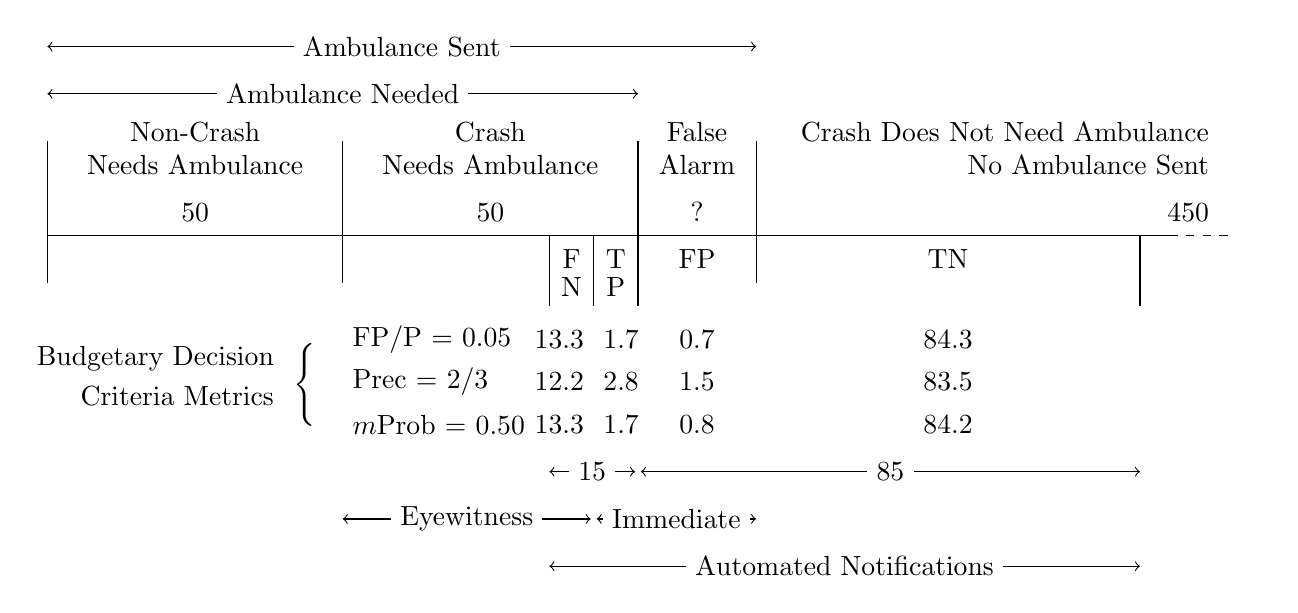
\begin{tikzpicture}[x=0.075cm, y=0.6cm, font=\normalfont\normalsize] % 15 cm wide


	\draw [<->, color=black]  (0,3) -- (100,3) 
		node [midway, color=black, fill=white, align=center] 
		{Ambulance Needed};

	\draw [<->, color=black]  (0,4) -- (120,4) 
		node [midway, color=black, fill=white, align=center] 
		{Ambulance Sent};


	\path (207,0) circle (0pt);
	\draw [color=black] (0,0) -- (190,0);
	\draw [color=black, dashed] (190,0) -- (200,0);
	\draw [color=black] (0,2) -- (0,-1);
	\draw [color=black] (50,2) -- (50,-1);
	\draw [color=black] (100,2) -- (100,-1.5);
	\draw [color=black] (120,2) -- (120,-1);
	\node (A) at (25,0) {};
	\node (B) [above=-2pt of A, align=center, text=black] {
		Non-Crash \\ Needs Ambulance \\[0.5em] 50
	};
	\node (C) at (75,0) {};
	\node (D) [above=-2pt of C, align=center, text=black] {
		Crash \\ Needs Ambulance \\[0.5em] 50
	};
	\node (E) at (200,0) {};
	\node (F) [above left =-2pt and 0pt of E, align=right, text=black] {
		Crash Does Not Need Ambulance \\ No Ambulance Sent \\[0.5em] 450
	};
	\node (G) at (110,0) {};
	\node (H) [above=-2pt of G, align=center, text=black] {
		False \\ Alarm \\[0.5em] ?
	};

	\draw [color=black] (85,0) -- (85,-1.5);
	\draw [color=black] (185,0) -- (185,-1.5);
%	\path (85,-2) -- (100,-2) node [below, midway, color=black] {15};
%	\path (100,-1) -- (185,-1) node [below, midway, color=black] {85};
	
%	\node (G) at (110,2) [color=black, align=left] {False \\  Alarm};
	\path (100,-0.5) -- (120,-0.5) node [midway, color=black] {FP};
	\path (120,-0.5) -- (185,-0.5) node [midway, color=black] {TN};
	\draw [color=black] (92.5,0) -- (92.5,-1.5);
	\path (85,-0.5) -- (92.5,-0.5) node [midway, color=black] {F};
	\path (85,-1.2) -- (92.5,-1.0) node [midway, color=black] {N};
	\path (100,-0.5) -- (92.5,-0.5) node [midway, color=black] {T};
	\path (100,-1.2) -- (92.5,-1.0) node [midway, color=black] {P};
	
	\node () at (50,-2.2) [right, color=black] {FP/P = 0.05};
	\node () at (92.5,-2.2) [left, color=black] {13.3};
	\node () at (92.5,-2.2) [right, color=black] {1.7};
	\node () at (110,-2.2) [color=black] {0.7};
	\node () at (152.5,-2.2) [color=black] {84.3};

	\node () at (50,-3.1) [right, color=black] {Prec = 2/3};
	\node () at (92.5,-3.1) [left, color=black] {12.2};
	\node () at (92.5,-3.1) [right, color=black] {2.8};
	\node () at (110,-3.1) [color=black] {1.5};
	\node () at (152.5,-3.1) [color=black] {83.5};

	\node () at (50,-4) [right, color=black] {$m$Prob = 0.50};
	\node () at (92.5,-4) [left, color=black] {13.3};
	\node () at (92.5,-4) [right, color=black] {1.7};
	\node () at (110,-4) [color=black] {0.8};
	\node () at (152.5,-4) [color=black] {84.2};
	
	\node () at (40,-2.6) [left, color=black] {Budgetary Decision};
	\node () at (40,-3.4) [left, color=black] {Criteria Metrics};

%	\node () at (50,-3.2) [left, color=black] {$\displaystyle \Biggl\{$};


	\node () at (40,-3.2) [right, color=black] {
		$\displaystyle 
			\left\{
			\vrule width 0pt height 14pt depth 14pt
			\right.
		$
	};

	\draw [<->, color=black]  (100.5,-5) -- (185,-5) 
		node [midway, color=black, fill=white, align=center] 
		{85};

	\draw [<->, color=black]  (85,-5) -- (99.5,-5) 
		node [midway, color=black, fill=white, align=center] 
		{15};

	\draw [<->, color=black]  (50,-6) -- (92,-6) 
		node [midway, color=black, fill=white, align=center] 
		{Eyewitness};

	\draw [<->, color=black]  (93,-6) -- (120,-6) 
		node [midway, color=black, fill=white, align=center] 
		{Immediate};

	\draw [<->, color=black]  (85,-7) -- (185,-7) 
		node [midway, color=black, fill=white, align=center] 
		{Automated Notifications};

	

	
\end{tikzpicture}








\caption{\normalfont\normalsize Springfield after implementing immediate dispatch of ambulances.  Figure accompanies \S\ref{scenario_reprise}}
\label{intro_springfield_conclusion}
\end{figure}

\FloatBarrier

Should Springfield implement such an AI recommendation system for immediate dispatch of ambulances based on automated notifications from cell phones?  If the only cost were the ambulances falsely dispatched (FP), then probably yes.  Considering the fixed costs of implementing such a system, a smaller city would have other options of programs that can better improve health and save more lives with the same amount of money.  

Springfield should consider changing the values of the metrics, perhaps to allow a FP/P = 10\% increase in the number of ambulances sent to automated crash notifications.  The best model on the Hard features, however, would give TP = 2.9 and FP = 1.5, more than doubling the cost (FP) without doubling the benefit (TP) from FP/P = 5\% with TP = 1.7 and FP = 0.7.  As we saw in our model output histograms, the returns diminish very quickly.  

With better data and more appropriate model algorithms, of course, we might get models that do a better job of separating the negative and positive class, an opportunity for future research.  (See \S \ref{simplifying_assumptions})

%%%%%
\subsection{Discussion}

Choosing a tradeoff between saving lives and saving money is a fraught political question, but the decisions can be informed with models showing the likely outcomes of the possible choices.  

Many cell phones can automatically notify the emergency dispatcher when they detect the deceleration profile of a crash.  The dispatcher will immediately send police to investigate, but should they also immediately dispatch an ambulance, which has about a small chance of being needed, or wait for a call from an eyewitness?  We have explored options for an AI recommendation system that would take the known information about the crash, a model built on historical crash data, and a decision criterion chosen by the political decision makers, and return a recommendation for whether to immediately dispatch an ambulance or to wait for a call from an eyewitness.

The main problem with such a recommendation system is that it will recommend sending some ambulances that are not needed.  Budgets are limited, and priorities have to be chosen.  We showed how to incorporate three kinds of decision criterion:  Percent increase in number of ambulance calls, percent of immediately dispatched ambulances actually needed, and minimum probability that each immediately dispatched ambulance is needed.  

We considered many challenges, including the randomness inherent in machine learning models and how the numerics severely limit the precision we can claim in our results.  Another challenge is identifying with useful numerical precision the decision threshold $\theta$ that satisfies a given metric when the value of that metric is only stable after much smoothing.  We found that finding $\theta$ for the first metric, a cap on increased ambulance runs, is straightforward, but Precision requires some smoothing, and marginal probability that an ambulance is needed is very unstable on small intervals.

The most significant challenge of implementing such a system is the cost and availability of the input data required to make a useful recommendation system.  We considered three sets of input features that we called Easy, Medium, and Hard, but that can also be thought of as Free, Expensive, and Problematic.  Even through the randomness and numerics, the results show that the results of models built on the Hard features are clearly better than those built on the Medium features, which are clearly better than those built on the Easy features.  The models built on the Easy features, however, are still better than random guessing, and a recommendation system built on just those features may be worth the expense, especially since the emergency dispatcher already has that information.  







%%%%% Future Work
\section{Simplifying Assumptions and Opportunities for Future Research}
\label{simplifying_assumptions}

All models are simplifications, and we should acknowledge the most egregious of our simplifying assumptions.  Some of the simplifying assumptions may hint at opportunities for future research.  

\

\begin{tabular}{rp{5in}}
%\begin{longtable}{rp{5in}}
	\bf Section & \bf Simplifying Assumption \cr \hline
	\S\ref{political_decisions} & All ambulances sent based on calls from eyewitnesses are actually needed. \cr
	& All automated crash notifications from cell phones refer to an actual crash, not just hard braking, {\it i.e.} the notifications have no false positives. \cr
	\S\ref{dataset} & The class ratio (P/N) in the automated crash notification from cell phones will be close to that in the CRSS data, $1/5$. \cr
	\S\ref{dataset} & The crash persons in the CRSS data are representative of the future crash persons whose cell phones send a crash notification.  (Several layers to unpack here) \cr
	\S\ref{features} & The data features we seek for each automated crash notification will be available and accurate. \cr
\end{tabular}	
%\end{longtable}


\

\begin{tabular}{rp{5in}}
%\begin{longtable}{rp{5in}}
	\bf Section & \bf Opportunities for Future Research \cr \hline
	\S\ref{dataset} & Find data on crashes that spawned an automated notification from a cell phone. \cr
	\S\ref{features} & We tested only three sets of features and did not test to see which features or combinations of features were most useful in predicting needing an ambulance.  \cr
	\S\ref{hyperparameters} & We found that varying the hyperparameters for class weight and focal loss did not significantly vary the ROC AUC, a measure of how well the model separates the positive and negative classes over the whole range $p \in [0,1]$.  Do those hyperparameters make a difference in how well the model separates the positive and negative classes on the right tail of the $p$ distribution, the part relevant to our work? \cr
	\S\ref{finding_theta} & Find a better way to slice the $p$-values into intervals such that the target metrics are monotonic functions of the intervals.  \cr
	\S\ref{scenario_reprise} & Can we find better combinations of data and model algorithms that will better separate the positive and negative classes? \cr
\end{tabular}	
%\end{longtable}




%%%%%
\section*{Funding Statement}

This research did not receive any specific grant from funding agencies in the public, commercial, or not-for-profit sectors.

%%%%% Conflict of Interest
\section*{Conflict of Interest}

Declarations of interest: none
%The authors have no relevant financial or non-financial interests to disclose.

%%%%% Acknowledgements
\section*{Acknowledgements}

George Broussard 
%[STUDENT]
contributed to this work in the 
%[FUNDED PROGRAM]
NSF Research Experiences for Undergraduates program.

%%%%% Data Availability
\section*{Data Availability}

The CRSS data is publicly available at 

\url{https://www.nhtsa.gov/crash-data-systems/crash-report-sampling-system}

All of the code and generated data, tables, and graphs are available at 
\url{http://www.github.com/bburkman/Ambulance_Dispatch}

%%%%% Declaration of Generative AI and AI-assisted technologies in the writing process
%\section*{Declaration of Generative AI and AI-assisted technologies in the writing process}



\begin{comment}
% Figure
\begin{figure}[<options>]
	\centering
		\includegraphics[<options>]{}
	  \caption{}\label{fig1}
\end{figure}


\begin{table}[<options>]
\caption{}\label{tbl1}
\begin{tabular*}{\tblwidth}{@{}LL@{}}
\toprule
  &  \\ % Table header row
\midrule
 & \\
 & \\
 & \\
 & \\
\bottomrule
\end{tabular*}
\end{table}
\end{comment}

% Uncomment and use as the case may be
%\begin{theorem} 
%\end{theorem}

% Uncomment and use as the case may be
%\begin{lemma} 
%\end{lemma}

%% The Appendices part is started with the command \appendix;
%% appendix sections are then done as normal sections
%% \appendix

%\section{}\label{}

% To print the credit authorship contribution details
\printcredits

%% Loading bibliography style file
%\bibliographystyle{model1-num-names}
\bibliographystyle{cas-model2-names}

% Loading bibliography database
\bibliography{Ambulance_Dispatch.bib}

\begin{comment}
% Biography
\bio{}
% Here goes the biography details.
\endbio

\bio{pic1}
% Here goes the biography details.
\endbio
\end{comment}

\end{document}

